% Created 2017-03-27 Mon 14:15
% Intended LaTeX compiler: pdflatex
\documentclass[12pt,oneside]{cmuthesis}
\usepackage[utf8]{inputenc}
\usepackage{lmodern}
\usepackage[T1]{fontenc}
\usepackage{graphicx}
\usepackage{longtable}
\usepackage{float}
\usepackage{wrapfig}
\usepackage{rotating}
\usepackage[normalem]{ulem}
\usepackage{amsmath}
\usepackage{textcomp}
\usepackage{marvosym}
\usepackage{wasysym}
\usepackage{amssymb}
\usepackage[superscript]{cite}
\usepackage[version=3]{mhchem}
\usepackage{url}
\usepackage{minted}
\usepackage{underscore}
\usepackage[linktocpage,pdfstartview=FitH,colorlinks,
             linkcolor=blue,anchorcolor=blue,
             citecolor=blue,filecolor=blue,menucolor=blue,urlcolor=blue]{hyperref}
\usepackage{times}
\usepackage{fullpage}
\usepackage{titlesec}
\usepackage[letterpaper,bindingoffset=1in,
            left=1in,right=1in,top=1in,bottom=1in]{geometry}
\usepackage[nottoc,numbib]{tocbibind}

\titleformat{\chapter}[block]
   {\normalfont\Large\bfseries}{\thechapter. }{0pt}{\Large}
\author{Jacob Russell Boes}
\date{April, 2017}
\title{Multiscale Modeling of Adsorbate Interactions on Transition Metal Alloy Surfaces}
\begin{document}

\maketitle

\frontmatter
\previousdegrees{B.S., Chemical Engineering, Michigan Technological University}

\begin{abstract}
Transition metals represent some of the first catalysts used in industrial processes and are still used today to produce many of the most needed chemicals. Adopting from ancient metallurgical techniques, it followed that the performance of these basic transition metals can be refined by adding multiple components. Since that time, improvements to these alloy catalysts has been mostly incremental due to the difficulty of producing new catalysts experimentally and a lack of fundamental understanding of the underlying physics.

More recently, computational chemistry has proven itself an increasingly effective means for identifying these underlying physics. Through the use of $d$-band interactions of adsorbates with the surface, basic adsorption characteristics can be predicted across transition metals with limited initial information. However, although these models function well as high-level screening tools, much work is yet to be done before optimal catalysts can be comfortably designed from properties which experimentalists can directly control. This remains particularly challenging for alloy modeling, primarily due to the large number of possible atomic configurations, even for two metal systems.

This work focuses on developing the methods for modeling optimal reaction properties at the surface of a transition metal alloy. Based on thermodynamic equilibrium between the surface, bulk, and gas reservoir, a model for the prediction of segregation under vacuum and adsorbate conditions can be predicted. Furthermore, by relating strain in the bulk lattice constant to the adsorption energies of varying local active sites, the optimal surface compositions can be related to bulk composition; a feature which can easily be selected for. Although useful for identifying trends across bulk composition space, these methods are limited to a small subset of active site configurations.

To capture the complexity of more sophisticated processes, such as segregation, higher-timescale methods are required. Traditional computational tools are often too expensive to implement for these methods, and as such, they are usually completed with less-accurate potentials. In this work, we demonstrate that machine learning techniques have improved accuracy compared to physical potentials. We then go on to demonstrate how this improved accuracy can lead to experimentally accurate predictions of segregation.
\end{abstract}

\begin{acknowledgments}
I write this dissertation in recognition of all of the educators who devoted their time to help propel me to this point. Without their support none of this work would have been possible. I would like to especially thank my academic advisor, John Kitchin, whose model has inspired me to pursue a career in research, a position in which I feel I can best do my part to help improve the quality of others lives, the same way he has done for me.

Special thanks to my thesis committee for participating in the dissertation process: \\
John Kitchin, Chair \\
Andrew Gellman \\
Mike Widom \\
Erik Yidste
\end{acknowledgments}

\tableofcontents
\listoftables
\listoffigures

\mainmatter
\renewcommand{\baselinestretch}{1.66}\normalsize

\chapter{Introduction}
\label{sec:ch0}
In the future, all fields of science will follow the same progression as what has been seen in physics. As our understanding of the sciences continues to grow, experimental procedures will become increasingly complex, expensive, and difficult to perform. In contrast, computer performance continues to double every two years in accordance with Moore's law \cite{schaller-1997-moores-law}. This continued advancement in computational power allows for increasingly expensive techniques to be implemented using ever-improving atomistic potentials which describe the underlying chemistry \cite{boes-2016-neural-networ,perdew-2005-presc-desig}. As such, computational insights play an important role in understanding the underlying physics of catalysis and surface science. As our understanding of the underlying physics improves, so too does our ability to design increasingly favorable catalysts without the needs for guess work. This leads us towards the ultimate goal of designing catalysts entirely from simulation.

As the accuracy of potentials increases, so too does their computational cost. Ideally, only the most accurate potentials would be utilized at all levels of theory. However, even with improved computational performance, only certain levels of theory are feasible depending on the level of sophistication required in the methods. This is the crux of multi-scale modeling, represented graphically in Figure \ref{fig-multiscale}.

\begin{figure}[h]
\centering
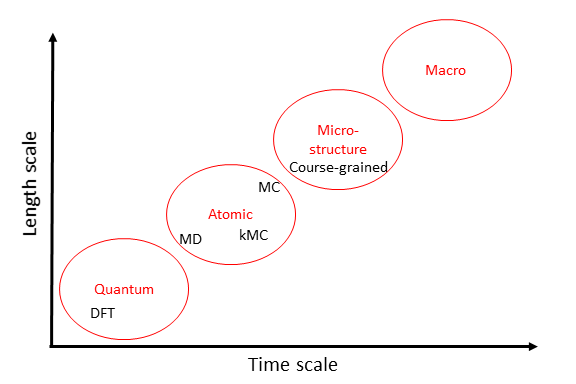
\includegraphics[width=5.5in]{./images/fig-multiscale.png}
\caption{Diagram of multiscale modeling in the context of reaction simulation in catalysis. General categories of time-scale are marked in red. Some of the methodologies utilized in this dissertation are marked in black. \label{fig-multiscale}}
\end{figure}

Each time scale in Figure \ref{fig-multiscale} represents a different set of methodologies used to adequately model the physics at each associated length scale. As engineers, we are ultimately only interested in the smallest possible scale that can be controlled experimentally. For most chemical operations, that is the macro-scale. Never the less, we are interested in the quantum-level chemistry because all higher-level methods stem from the underlying physics at the smallest time scales. Without a complete understanding of surface chemistry at the quantum level, there is little hope of intelligently designing the best possible catalysts for any given reaction from scratch. Based on this understanding, there is a need to help bridge the gap between time scales, which will allow for accurate representation of more complex chemistry. This improvement is particularly relevant to the study of transition metals alloys; difficult systems to study, due to the large number of potentially relevant configurations.

The objective of this dissertation is to outline advances in alloy simulation techniques spanning the electronic and atomic time scales. The ultimate goal of which is to be able to develop a method for the prediction of a bulk composition of an alloy which will optimize a given surface reaction, entirely from simulation. In Chapter \ref{sec:ch1}, we summarize the difficulties of alloy simulation, with reference to the electronic and atomic time-scales. Chapter \ref{sec:ch2}, discusses previously published work \cite{boes-2015-estim-bulk} outlining a computationally cost-effective coarse-grained model for determining bounded attributes of surface chemistry. This process is demonstrated for the prediction of hydrogen adsorption onto a CuPd(111) surface.

The second half of this dissertation (Chapters \ref{sec:ch3}-\ref{sec:ch6}), discusses new developments in machine-learning based atomic potentials for retaining electronic accuracy at atomic scales. Chapter \ref{sec:ch3} provides a brief overview of various forms of atomic potentials. These potentials are critical to the Monte Carlo and molecular dynamics techniques, which are required to simulate longer time-scales. Chapter \ref{sec:ch4} covers previously published work \cite{boes-2016-neural-networ} comparing a popular physical potential, known as ReaxFF, with the newer machine-learning based potentials. Here we show that the machine-learning neural network (NN) based potentials \cite{behler-2007-gener-neural} are very promising tools for highly-accurate predictions of various transition metal systems. Chapters \ref{sec:ch5} and \ref{sec:ch6} cover previously published work \cite{boes-2017-neural-networ,boes-2017-model-segreg} expanding the application of these neural network potentials to coverage-dependent adsorption interaction of oxygen on Pd and AuPd segregation under vacuum conditions. Finally, the dissertation concludes in Chapter \ref{sec:ch7} with a summary of this work and future research directions.

\chapter{Alloy Modeling Complexities and Methods}
\label{sec:ch1}
\section{Introduction to Transition Metal Alloy Simulation}
\label{sec:org2d66271}
Transition metals have a long and important history in the field of heterogeneous catalysis, being one of the most obvious choices as an electron transfer medium. They exist in many of the most important reactions, including the famous Haber-Bosch process \cite{liu-2014-ammon-synth} used to synthesize ammonia, water splitting, the production of ethylene, and many others \cite{greeley-2004-alloy-catal,zhang-2016-homog-disper}.

Alloys are frequently used in catalysis because they allow for tailoring of catalytic properties from those of their component metals \cite{ponec-2001-alloy-catal,yu-2012-review-pt}. For example, AuPd is favorable for hydrogen peroxide synthesis from H\(_{\text{2}}\) and O\(_{\text{2}}\) \cite{landon-2003-direc-synth}. Pd alone catalyzes both hydrogen peroxide formation and the undesirable secondary step of its decomposition into H\(_{\text{2}}\)O. By alloying with Au, the decomposition step can be mitigated, leading to higher selectivity \cite{edwards-2009-switc-off,plauck-2016-activ-sites}. This fine-tuning of desired behavior leads to questions of what the best ratio of component materials is to obtain the best result; Au itself is not very active, yet Pd catalyzes an undesirable reaction. Clearly an optimal surface composition must exist that maximizes the selectivity.

Computational catalysis has made many contributions to understanding the reactivity of alloy active sites for designing such superior catalysts. However, computational methods can only be incorporated into catalyst design when the structure and composition of the sites are known \cite{kitchin-2008-densit-funct}. Under these circumstances, we can readily estimate the reactivity of a site \cite{greeley-2005,inoglu-2010-new-solid}. However, significant challenges remain when modeling alloy catalysts. A real alloy surface will have a distribution of sites with different compositions. Many different possible active site geometries exist as well depending on how the surface is formed, each with their own properties. The metal atoms that exist in the alloy are also likely to be different sizes, causing strain on the bulk and surface structures away from the lattice constants typical to the pure components. Identifying which phases are present in the bulk is also critical for determining the relevant models to construct, as determined from phase diagrams \cite{geng-2017-first-princ}.

Furthermore, the composition of an alloy surface is not likely to be the same as that of the bulk alloy, since the atoms at the surface reside in a much different chemical environment from the bulk. The preference for on of the metals in the alloy to prefer to exist at the surface is known as segregation \cite{dowben-1990-surfac-segreg-phenom}. The surface composition will further depend on the gas-phase environment as well \cite{kitchin-2008-alloy}. Thus, although it is simple to model the properties of a single site, or even many sites, identifying \emph{what} site(s) to model and how significant they are under reaction conditions remains a great challenge. It is also difficult to determine the properties of the ensemble of sites, or how they interact in models of higher time-scales to produce the properties of interest, such as activity and selectivity.

Experimentally, segregation has typically been measured one bulk composition at a time \cite{chen-2006-natur-activ,bocarme-2009-surfac-segreg,haire-2011-influen-prepar} using a method such as low-energy ion scattering spectroscopy (LEISS). These experiments are time-consuming leading to limited experimental results at a few bulk compositions and temperatures. Although there are growing efforts experimentally to measure segregation profiles at clean alloy surfaces with high-throughput techniques \cite{miller-2008-surfac-segreg,priyadarshini-2011-high-throug} these results may have limited value under reaction conditions where adsorbate-induced segregation has been observed \cite{kitchin-2008-alloy,menning-2009-gener-trend,kim-2013-co-adsor}. Surface reaction characteristics can also be measured in a high-throughput fashion using micro-kinetic models \cite{gumuslu-2015-correl-elect}, but without an underlying understanding of the physics, selection of alloys must be performed via trial and error. The development of validated computational approaches to estimate surface compositions in alloys is invaluable.

As mentioned previously, specific site structures and compositions are modeled in typical studies of adsorption on alloy surfaces \cite{alfonso-2003-densit-funct,greeley-2009-combin-densit}. These studies are valuable, but they can be difficult to connect directly to experiments because the compositions modeled are often not the same as the experimental compositions; for example, due to segregation effects. While many methods exist that qualitatively predict segregation behavior \cite{ruban-1999-calcul,skriver-2000-steps,nilekar-2009-surfac,han-2009-step-decor} these guidelines focus on the dilute limit, and it has been a challenge to quantitatively model segregation across composition space and under reaction conditions. Some progress in this has been made for AuPd alloys \cite{soto-verdugo-2007-segreg-at,atanasov-2009-equil-order,creuze-2015-surfac-segreg}, although the results are often derived from lower-accuracy potentials. In chapter \ref{sec:ch6}, we focus on more accurate methods to quantitatively model segregation across composition space in the absence of adsorbates. A critical component for the prediction of optimal reactivity under reaction conditions.

State of the art modeling of alloy surfaces that incorporates segregation from the bulk, adsorption on the surface, and the reactive conditions relies on 2 key components: 1) An atomic potential -- such as density functional theory (DFT) -- which takes a set of atomic positions as inputs and provides energies as an output, and 2) a computational method for an appropriate time-scale. Some examples of formerly state of the art methods include DFT with thermodynamic models \cite{kitchin-2008-alloy} and cluster expansions with Monte Carlo techniques \cite{han-2005-surfac-segreg,mei-2009-hydrog-acety}. Both of these examples, although thermodynamically rigorous, are very computationally demanding and come with limitations. This difficulty is primarily due to the large number of possible configurations that must be considered. Accurate \emph{ab-initio} methodologies such as DFT are often too computationally intensive to be used directly. Atomistic potentials such as ReaxFF have been used \cite{kwak-2012-ab-initio}, but these approaches often compromise accuracy for speed \cite{boes-2016-neural-networ}. A DFT-based approach using cluster expansions has been used to model segregation in an alloy surface \cite{han-2005-surfac-segreg,welker-2010-predic-segreg}, but these simulations are difficult to extend, and the codes for performing them are not readily available.

In the following sections of this chapter, we go into brief discussion of the various time-scale methodologies mentioned above and displayed graphically in Figure \ref{fig-multiscale}. Development of superior atomic potentials is central to the advances made in this dissertation and are discussed in greater detail in Chapter \ref{sec:ch3}.

\section{The Quantum Scale: Density Functional Theory}
\label{sec:orgb6d33c0}
For the purposes of catalysis, the quantum time-scale is the smallest and consequently provides the greatest level of detail about a system of atoms. Our understanding of these atomic systems is derived from the Schrödinger equation \cite{pauling-1985-introd-quant}. This equation is an eigenvalue problem which describes the underlying physics of an atomic system in its entirety, down to the interactions between the electrons themselves. However, due to its complex nature, an exact solution to the Schrödinger equation can only be derived for a system with a single electron. Therefore, to make use of this powerful tool, a numerical solution is required.

A popular choice for this is DFT, which solves the non-interacting portion of this many-electron problem exactly. The contribution to the energy of a system from the exchange and correlation of electrons is then approximated by a functional. Various choices of these functional are associated with different levels of theory and determine the overall accuracy of the calculations. However, as the level of theory increases, the computational cost of performing these calculations increases as well. This concept is similar to that of the trade-offs in cost and energy of lower-level atomic potentials as well, as discussed in Chapter \ref{sec:ch3}. These potentials also provide valuable insights about the way transition metal electrons interact with those of adsorbates. In fact, some of the most powerful trends across transition metal-adsorbate interactions have been born of these interactions in the form of the \emph{d}-band model \cite{hammer-1995-why-gold,hammer-2000-theor}.

Energies calculated using quantum-based potentials are the most accurate and are thus typically considered the gold-standard across all time-scales. However, they are also very expensive, taking a few days to a week to calculate even the smallest surface interactions of interest. This quickly becomes computationally infeasible when attempting to determine many of the necessary aspects of a catalyst needed to accurately simulate catalysis at a macroscopic level. In the absence of limited computational recourse, all of the methods in subsequent sections would be performed with the highest level of theory. It is also worth noting that as computers become increasingly powerful, these high-level methods will become increasingly available to longer time-scale simulations.

\section{The Atomic Scale: Molecular Dynamics and Monte Carlo}
\label{sec:org7cf6431}
Adsorption onto a metal surface is a critical step in heterogeneous catalysis since it is often a precursor to subsequent reactions. The properties which define the rates of these surface reactions, such as adsorption energies and diffusion barriers, are key to creating predictive models of existing catalytic technology. These adsorbate interactions with the metal surface are determined by the underlying potential energy surface (PES). In the case of dynamic surfaces, these PESs have many dimensions from the presence of multiple adsorbates and also as a result of thermally excited metal atoms. This high-dimensionality makes obtaining a complete picture of the PES difficult for standard \emph{ab-initio} techniques, such as DFT, which rely upon discrete sampling.

The concept of the PES becomes important to understand once we wish to move our atomic simulations to a finite temperature; a feature which is foreign to quantum-level calculations, which are performed at 0 K. The incorporation of temperature into the simulation dramatically increases the complexity. Many additional states become accessible to a given system of atoms with the nuclei in motion. However, understanding the underlying trends in these newly accessible states is the key to our understanding of adsorption under reaction conditions \cite{rogal-2007-ab-initio,shi-2007-first-princ}.

Fortunately, the path to understanding the progression of a system of atoms is clear. At finite temperatures, each atom will have a momentum associated with that temperature at any given point in time. These momentum, when combined with the underlying interactions between the atoms, represent a force for each atom in a specific direction. By progressing time forward in small increments, we can see how the system of atoms naturally evolves.  This process of progressing the positions of the atoms iteratively through time is known as molecular dynamics (MD) \cite{haile-1992-molec}. Since the forces on the atoms are dependent upon their position, which change with time, it is important that the time-increment for this process remain small to prevent error in the calculation of the positions. It is this necessarily small time-increment that makes MD so computationally expensive. Furthermore, since each time step is dependent upon information from the last, these calculations must be performed serially. This often makes DFT and other \emph{ab-initio} techniques impractical for use in MD, although we wish to be as accurate as possible when exploring the PES.

At the atomic time-scale, we are often more interested in the positions of the atomic nuclei rather than the electrons surrounding them. Because of this, it is often deemed acceptable to use a lower-level atomic potential, incapable of describing the electronic interactions, but still able to represent the energies of the PES; ideally to the same level of accuracy. However, as discussed in Chapter \ref{sec:ch4}, even the most sophisticated of atomic potentials based on physical interactions between atoms often incur a significant loss of accuracy. This is the motivation for our work in Chapter \ref{sec:ch5} and \ref{sec:ch6}, where we explore alternative forms of atomic potentials.

While MD is incredibly useful, it can also be terribly inefficient depending on the desired result. This is due to the fact that the MD trajectory (motion through time), includes a great deal of information about the kinetics of a process. While this kinetic information is critical to understanding all time-dependent aspects of the surface chemistry, there are also many cases in which it is acceptable simply to understand the thermodynamic, or the relative stability of distinctly different states. In this case, by assuming that each of these distinct states is kinetically achievable, we can simply compare the energies of these states directly and choose the most stable. Entropy contributions can even be incorporated in these models by occasionally accepting less-favorable states based on a Boltzmann distribution. This process of directly comparing different states is known generally as Monte Carlo (MC) sampling \cite{mooney-1997-monte}, and it can dramatically accelerate certain processes, such as the determination of equilibrium segregation states, as demonstrated in Chapter \ref{sec:ch6}. Note that this process also requires a good understanding of the possible states to sample.

Assuming that a process in not completely separate from the kinetics, it is also possible to utilize a hybrid of these two methods, known as kinetic Monte Carlo (kMC) \cite{binder-1986-introd}. In this case, the ``arc'' connecting the minimums in energy for each distinct group-state is also considered. By assuming the shape of the energy ``well'', that each energy minimum resides in, it is then possible to determine the average time required to escape one energy well into the other. By connecting all accessible states in this way, it is possible to recover time-dependent kinetic information about the system. It is important to note for this process that each obtainable state adjoining the current state must be considered simultaneously for this to work, making this process more computationally expensive than traditional MC and completely infeasible in some cases.

\section{The Micro-Structure Scale: Coarse-Grained and Micro-Kinetic Models}
\label{sec:org5dece4c}
Finally, the highest level of predictive model which will be discussed in this dissertation is the micro-structure scale. Here, we sacrifice the greatest amount of information yet to obtain the most important information regarding the selectively and reactivity of the catalyst. Micro-structure models are often characterized by their selective nature. Instead of considering all possible states, as we would with MC, now we will only consider a handful of the most relevant states, assuming that all others are inconsequential by comparison. As such, these methods often rely upon select calculations of more accuracy methods built into higher-level theory.

Due to the high-level nature of these frameworks, micro-scale models take many forms and can be difficult to classify. Microkinetic models are a common example \cite{carter-1961-kinet-model} based on transition state theory \cite{steinfeld-1989-chemic}. In surface science, these methods utilize some form of adsorption isotherm in conjunction with discrete thermodynamic and kinetic energies of the most important active sites and reaction barriers.

\chapter{Estimating Bulk-Composition-Dependent H\(_{\text{2}}\) Adsorption Energies on Cu\(_{\text{x}}\)Pd\(_{\text{1-x}}\) Alloy (111) Surfaces}
\label{sec:ch2}
In the previous chapter, we demonstrated that even the highest levels of theory rely upon input from the smallest time-scale simulations. As reactions become increasingly sophisticated and complex, so too must the integration of all levels of theory and simulation to create accurate models.

This chapter begins by addressing the complexities of predicting reaction properties of adsorbates on an alloy surface under reaction conditions at a micro-structure scale. This is demonstrated for H\(_{\text{2}}\) adsorption energies on a Cu\(_{\text{x}}\)Pd\(_{\text{1-x}}\) (111) surface. The work performed in this chapter has been published in Ref. \citenum{boes-2015-estim-bulk}, which includes additional supporting information (SI) outlining the details of all calculations and methods performed.

\section{Introduction}
\label{sec:org8496f6d}
In this chapter we outline a simple method to modeling adsorption behavior on heterogeneous alloy surfaces using DFT and statistical models. In this method we define a basis of adsorption sites which are likely to span the types of sites that will have the greatest impact on the adsorption energy. For each site, dissociative adsorption energies are then related to bulk composition using a relatively small set of DFT calculations. The probability of finding each active site at the surface is determined through a statistical distribution dependent on an arbitrary surface composition. The effective adsorption energy is then the sum of each sites adsorption energy times its probability of appearing on the surface. Finally, the surface composition is calculated by relating the Langmuir-McLean formulation of the Gibbs free isotherm to the experimentally determined vacuum segregation energy and an estimation of the segregation due to adsorbates.

The surface composition is estimated using experimental segregation data in conjunction with the calculated adsorption energies to estimate the surface composition under reaction conditions. Finally, the distribution of active sites is estimated from the surface composition and used to weight the calculated adsorption energies into the effective adsorption energy for the surface.

To illustrate this method we look specifically at the CuPd system which has been well studied experimentally due to its application as an extremely selective separator of H\(_{\text{2}}\) gas from syngas streams \cite{kamakoti-2005-predic-hydrog,obrien-2011-kinet-h,obrien-2012-h-d}. We prepared a composition spread alloy film (CSAF) \cite{fleutot-2012-appar-depos} mapping out the CuPd bulk composition space and determined the adsorption energy of H\(_{\text{2}}\) as a function of bulk composition through analysis of H\(_{\text{2}}\)-D\(_{\text{2}}\) exchange kinetics. We then compare our computationally-estimated bulk-composition dependent adsorption energies with these experimental results. Through this comparison we show that the method provides a reasonable approach for predicting chemical properties across bulk composition space. By studying deviations in adsorption energy predictions from those measured, the method also allows for a more detailed understanding of the surface characteristics at the atomic level.

\section{Methods}
\label{sec:org32ce6b5}
\subsection{Experimental methods}
\label{sec:orga028d11}
H\(_{\text{2}}\)-D\(_{\text{2}}\) exchange kinetics across Cu\(_x\)Pd\(_{\text{1-}x}\) composition space using CSAF combinatorial materials libraries (shown schematically in Fig. \ref{fig-experiment}). CSAFs are thin alloy films with continuously variable lateral composition that are deposited onto compact substrates. We have previously reported the preparation and characterization of the CuPd CSAFs used in this work \cite{gumuslu-2015-correl-elect}. Briefly, an offset filament source \cite{priyadarshini-2011-high-throug,priyadarshini-2012-compac-tool} was used to deposit films of CuPd that are approximately 100 nm thick, with composition ranging from \(x = 0.3-1.0\), onto the surfaces of 14 mm \texttimes{} 14 mm \texttimes{} 2 mm polycrystalline Mo substrates; Figure \ref{fig-experiment} is a schematic diagram of the CSAF. After annealing the CSAF at 800 K, we used a unique multichannel microreactor \cite{kondratyuk-2013-micror-array} to measure the kinetics of H\(_{\text{2}}\)-D\(_{\text{2}}\) exchange at 100 discrete locations on the CSAF surface (indicated by the circles in Figure \ref{fig-experiment}) over a temperature range of 300-600 K and at various flow rates.

\begin{figure}[h]
\centering
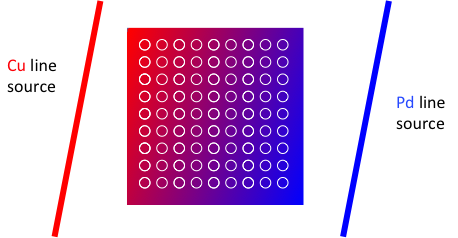
\includegraphics[width=3in]{./images/experiment.png}
\caption{Schematic representation of a Cu\(_x\)Pd\(_{\text{1-}x}\) CSAF. Cu (red) and Pd (blue) line sources are shown at the sides of the CSAF. Circles represent a 10 \texttimes{} 10 grid of microreactors distributed across the surface of the CSAF for kinetic measurements. \label{fig-experiment}}
\end{figure}

We previously reported a microkinetic model that we developed for interpretation of H\(_{\text{2}}\)-D\(_{\text{2}}\) exchange data \cite{obrien-2011-kinet-h}. The model is based on two elementary steps, dissociative adsorption of H\(_{\text{2}}\) (D\(_{\text{2}}\), HD) and recombinative desorption of H and D atoms to form HD (H\(_{\text{2}}\), D\(_{\text{2}}\)).  The model consists of a mass balance and a microkinetic expression for the rate of HD formation. We fit the model to the reaction data collected at each of the 100 locations on the surface of the CSAF to extract estimates of the adsorption (\(\Delta E^{\ddagger}_{ads}\)) and desorption (\(\Delta E^{\ddagger}_{des}\)) barriers. The adsorption energy is simply the difference between these two quantities (\(\Delta E^{H_{2}}_{ads} = \Delta E^{\ddagger}_{des} - \Delta E^{\ddagger}_{ads}\)).

\subsection{Computational methods}
\label{sec:org6df09a7}
All DFT calculations in this dissertation were performed using the Vienna ab-initio simulation package (VASP) \cite{kresse-1996-effic,kresse-1996-effic2} with the Perdew-Burke-Ernzerhof generalized gradient approximation (GGA-PBE) \cite{perdew-1996-gener-gradien,perdew-1997-gener-gradien} exchange-correlation functional. Core electrons were described using the projector augmented wave function (PAW) \cite{blochl-1994-projec-augmen,kresse-1999-from-ultras}.

In this chapter, \emph{k}-points were represented using Monkhorst-Pack grids \cite{monkhorst-1976-special-point} and the Kohn-Sham orbitals were expanded up to energy cutoffs of 425 eV for CuPd alloy models and 450 eV for PdH models. The Methfessel-Paxton scheme was used with a smearing parameter of 0.4 eV \cite{methfessel-1989-high-precis}. All calculations involving relaxations were completed with a force criteria \(< 0.05\) eV/\AA{}. Pure component lattice constants were determined using bulk calculations with \(12 \times 12 \times 12\) \emph{k}-point grids. Hydride bulk calculations were performed with \(8 \times 8 \times 8\) \emph{k}-point grids. Convergence studies of hydrogen adsorption energies computed with these parameters suggest the results are converged within \textpm{} 0.02 eV.

Alloy slab calculations were completed with \(8 \times 8 \times 1\) \emph{k}-point grids. The slab geometries were constructed with four metal layers, where the bottom two layers were fixed in place using various lattice constants between those of the pure components: 3.631 \AA{} for Cu and 3.952 \AA{} for Pd. The remaining two layers and the adsorbate were allowed to relax in the \emph{z}-axis. Hydride slabs were modeled as symmetric cells with a total of six metal layers, Pd terminated. The two center layers were fixed in place while the remaining two layers on either side were allowed to relax in the \emph{z}-axis. A \(10 \times 10 \times 1\) \emph{k}-point grid was used for these calculations. All slab geometries include 10 \AA{} of vacuum in the \emph{z}-axis. An extensive listing of all computational details is provided in the SI file of the published work \cite{boes-2015-estim-bulk}.

\section{Results and Discussion}
\label{sec:org4a08be0}
\subsection{Experimental determination of effective adsorption energies}
\label{sec:org942ac9f}
The measured adsorption (\(\Delta E^{\ddagger}_{ads}\)) and desorption (\(\Delta E^{\ddagger}_{des}\)) barriers are shown in Figure \ref{fig:exp-ads} over a large span of bulk compositions. Dissociative adsorption energies were calculated as \(\Delta E^{H_{2}}_{ads} = \Delta E^{\ddagger}_{des} - \Delta E^{\ddagger}_{ads}\). We do not show measured values of \(\Delta E^{\ddagger}_{des}\) at high \(x\) (\(> \; \approx 0.8\)) because their experimental uncertainties are large. For the calculation of \(\Delta E^{H_{2}}_{ads}\) throughout composition space, we use a linear fit of the \(\Delta E^{\ddagger}_{des}\) values measured at low \(x\). At high concentrations of Cu, \(\Delta E^{H_{2}}_{ads}\) appears constant at approximately -0.3 eV (although the uncertainty here is large). As the amount of Pd in the alloy increases, \(\Delta E^{H_{2}}_{ads}\) becomes increasingly negative, until \(x \approx 0.6\), below which an increase in adsorption energy is observed.

\begin{figure}[h]
\centering
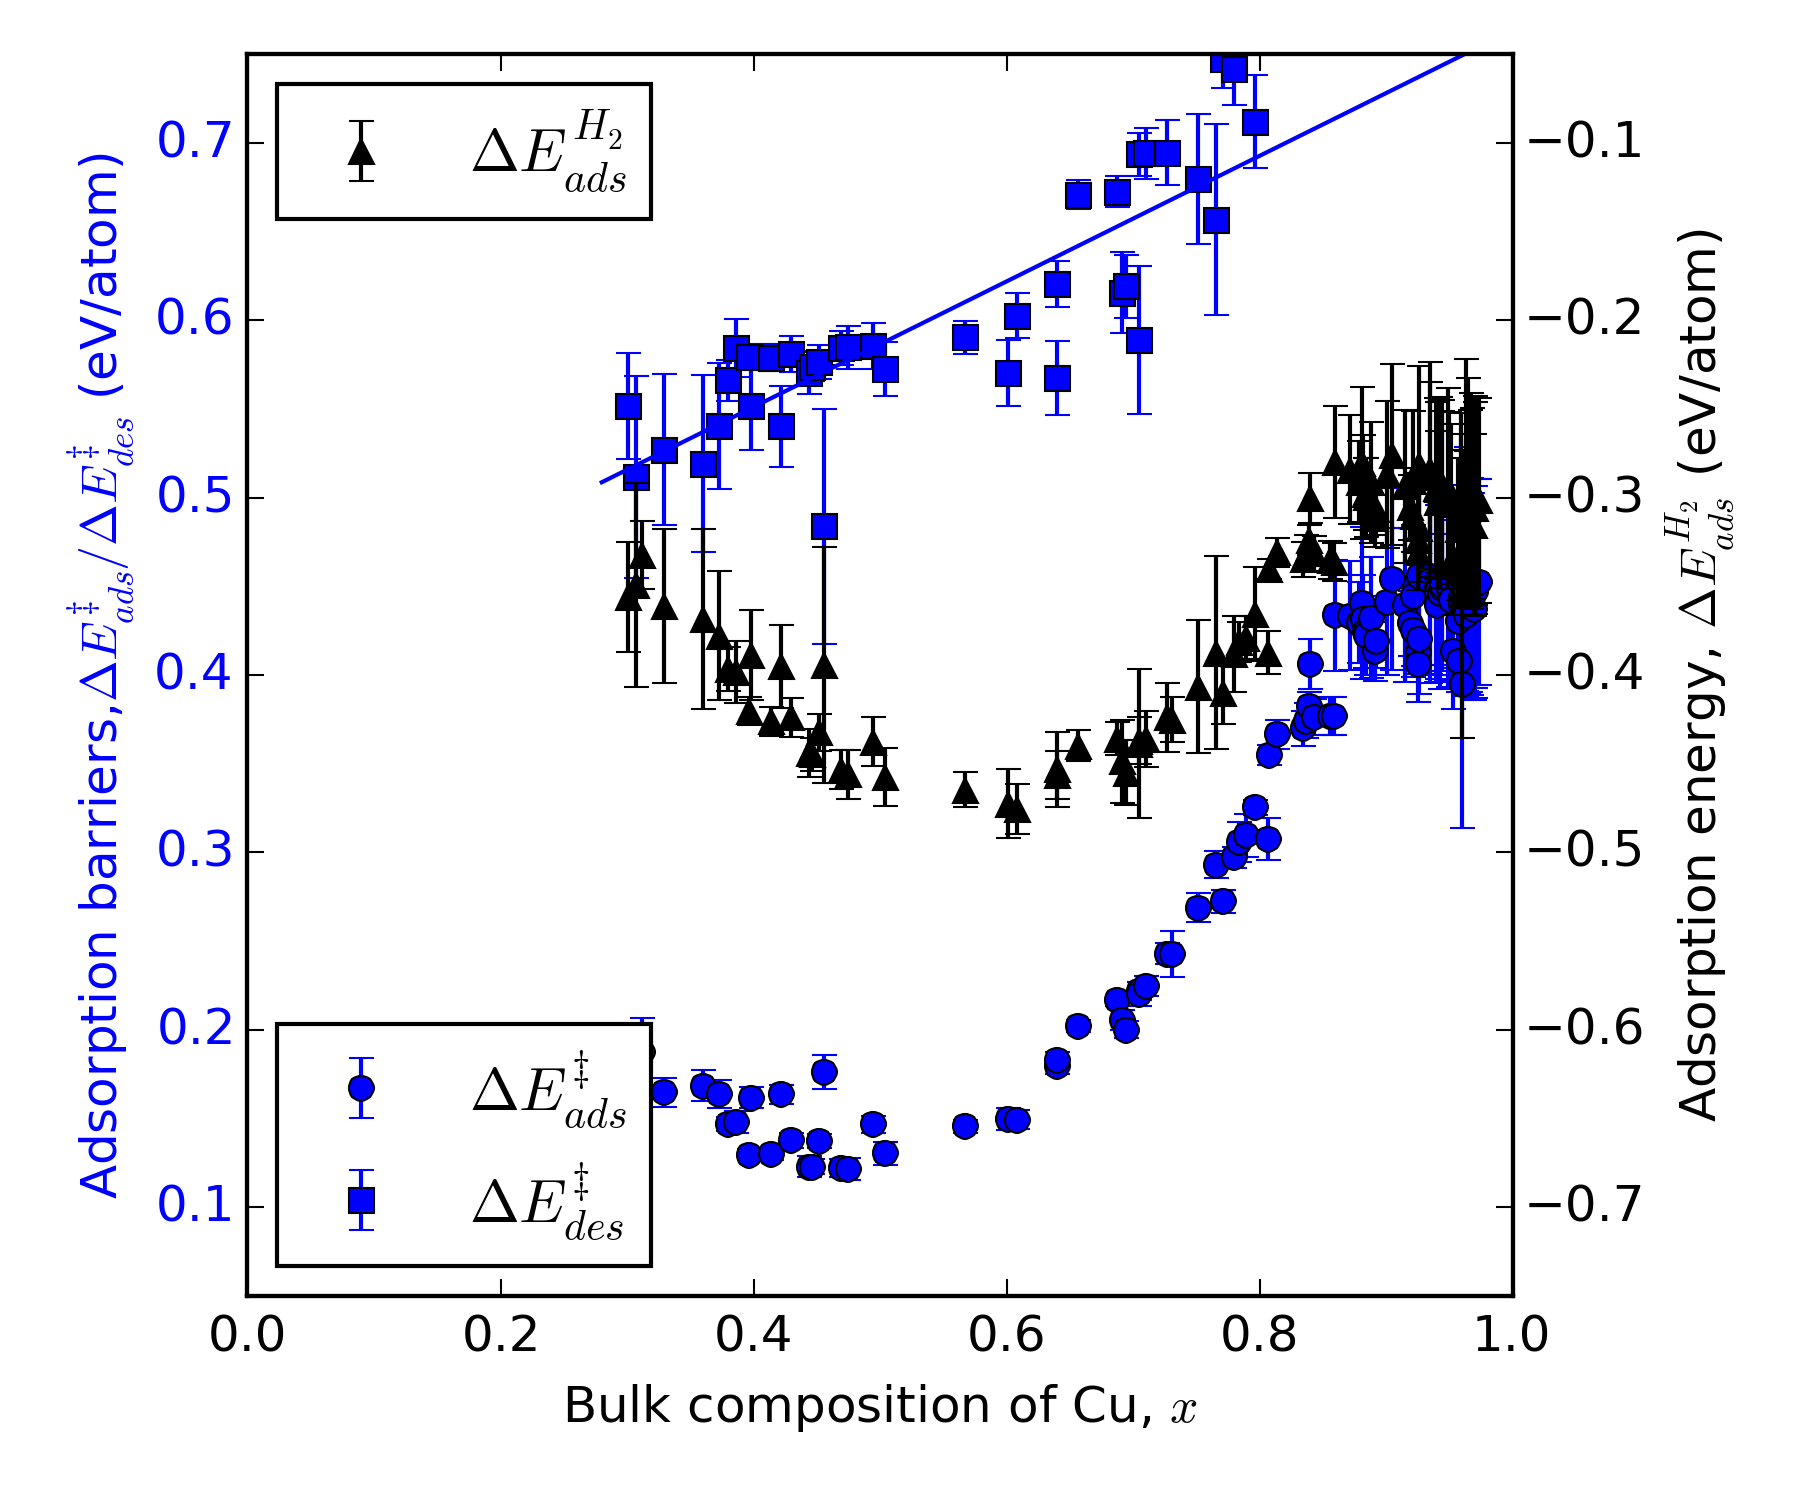
\includegraphics[width=5.5in]{./images/exp.png}
\caption{Experimental adsorption (\(\Delta E^{\ddagger}_{ads}\)) and desorption (\(\Delta E^{\ddagger}_{des}\)) barriers. Black triangles represent adsorption energies calculated as \(\Delta E^{H_{2}}_{ads} = \Delta E^{\ddagger}_{des} - \Delta E^{\ddagger}_{ads}\), where \(\Delta E^{\ddagger}_{des}\) values are based on the linear fit. \label{fig:exp-ads}}
\end{figure}

\subsection{Selection of the active site basis set}
\label{sec:org455d579}
Our strategy for computing an effective dissociative adsorption energy is to compute the adsorption energies of a basis of active sites, and then to average them in a suitably weighted way. The first step is identifying a basis of active sites on which to compute adsorption energies. The structure of the active sites is largely determined by the structure of the surface, which is in turn determined by the structure of the bulk. Based on the experimental phase diagram, \cite{dowben-1990-surfac-segreg-phenom,subramanian-1991-cu-pd-pallad} the CuPd system is in a disordered fcc bulk phase for the majority of the bulk composition space examined in this work; a B2 phase becomes stable between \(0.51 < x < 0.68\) at 800 K, the temperature to which the CSAF was annealed during preparation. We neglect the B2 phase in this work. We expect that the  fcc(111) orientation is predominant at the surface of the polycrystalline CSAF used in the experimental portion of this chapter \cite{obrien-2012-h-d}. Hence, we focus our modeling on the basis sites in an fcc(111) surface. Hydrogen adsorption energies were calculated on the fcc, hcp, bridge, and top sites of the pure component metals. The fcc adsorption site was found to be the most stable on each of the pure metal surfaces and it is assumed that this will be the case for all alloy compositions as well.

On the surface of an alloy, it is not clear what defines an adsorption site. A minimal site would be three atoms defining the fcc hollow position. However, there are ligand effects from atoms not directly adjacent to the adsorbate that influence the reactivity of those atoms. These effects tend to decay quickly with distance \cite{inoglu-2010-new-solid}. We seek a balance between the minimal number of atoms in a site that captures the dominant trends in activity but that are still enumerable. The minimum number of atoms needed to characterize an fcc site is three. For the fcc(111) surface of a CuPd alloy, this results in the four active sites shown in Figure \ref{fig-configs}. Only four sites are considered since rotations of the two mixed composition sites are assumed to have identical adsorption energies.

\begin{figure}[h]
\centering
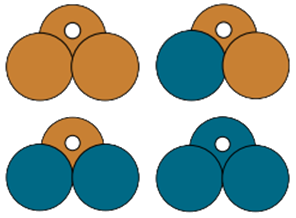
\includegraphics[width=2.5in]{./images/configs.png}
\caption{The four possible configurations of Cu (orange) and Pd (blue) atoms that can form fcc adsorption sites for hydrogen atoms. \label{fig-configs}}
\end{figure}

These sites must be embedded into an alloy slab for the adsorption energy to be calculated. It is not computationally feasible to model all possible slab compositions. Rather than attempt to mimic the alloy slab, we chose to embed these sites into pure Cu slabs and pure Pd slabs. This will mimic ligand effects on the embedded sites, and is likely to span the full range of these effects on the adsorption energies. Thus, we expect that this will provide bounds on the true adsorption energy for each site. This results in a total of eight unique slab compositions which were considered for the CuPd alloy portion of this chapter.

\subsection{Active site adsorption energies}
\label{sec:orgfbcd55a}
The next objective is to estimate the adsorption energy of a site that is embedded in a slab with properties of a bulk alloy of a given composition, e.g., at the lattice constant of the bulk alloy. We have to decide on the lattice constant that is appropriate for the calculation. In essence, we treat the slab as an effective medium that has an electronic structure similar to that of features as the alloy would have, so that we can estimate the adsorption energy of a site in that alloy.

The lattice constant of many alloys is often a linear function of bulk composition (Vegard's law \cite{denton-1991-vegar-law,bose-1992-elect-struc}). This trend  maps the lattice constant to the bulk composition space as shown in Equation \eqref{eqn-alpha}:

\begin{eqnarray}
\alpha(x) = (a_{Pd} - a_{Cu}) x + a_{Cu} \label{eqn-alpha},
\end{eqnarray}

\noindent
where \(\alpha\) is the alloy lattice constant, \(a_{M}\) is the lattice constant of pure component metal \(M\). We can readily verify this trend computationally using cluster expansion methods of the stable ground state configurations of the alloy \cite{walle-2002-self-monte,walle-2002-autom}. The resulting ground state configurations from a cluster expansion of the CuPd system are shown in Figure \ref{fig-vegard}. Additional details regarding cluster-expansion techniques can be found in Chapter \ref{sec:ch3}. The lattice constants of the ground state configurations vary linearly with alloy composition. This is in good agreement with Vegard's law. Thus, we use Equation \eqref{eqn-alpha} to determine the slab lattice constant for any given bulk composition.

\begin{figure}[h]
\centering
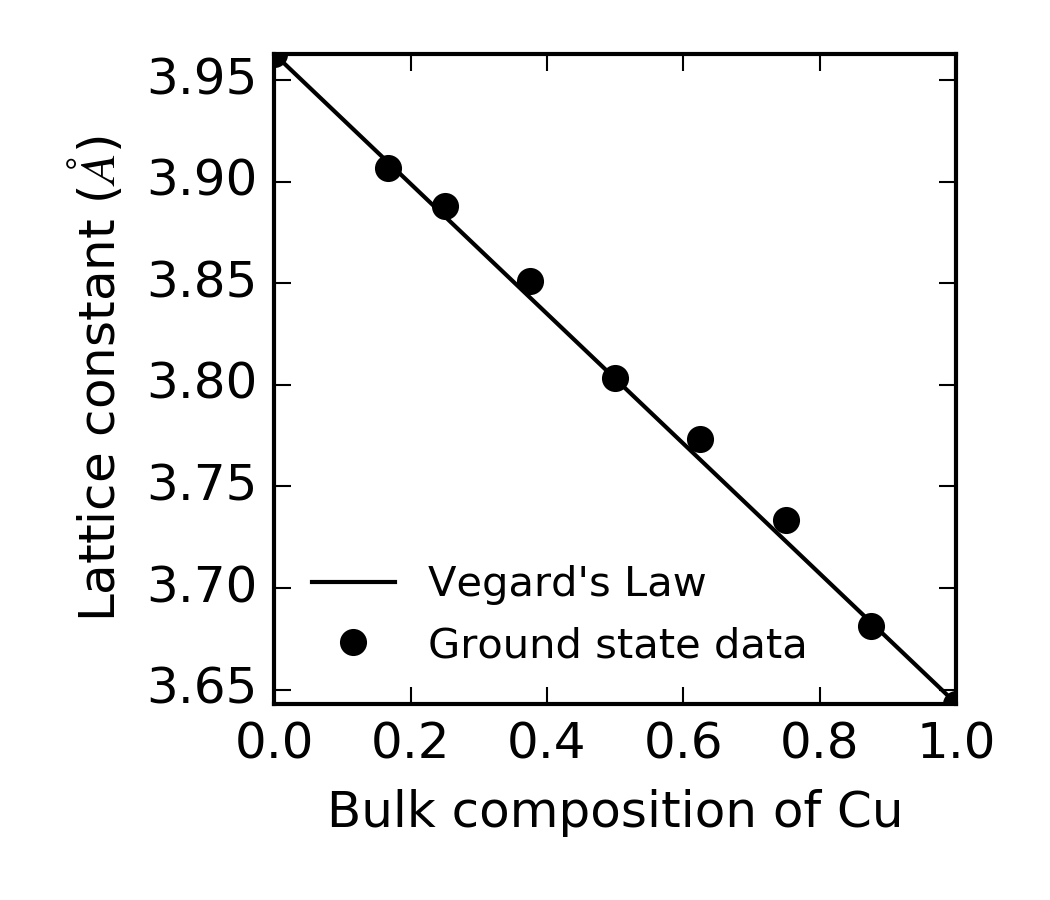
\includegraphics[width=3.5in]{./images/vegard.png}
\caption{Lattice constants of the ground state fcc CuPd configurations plotted with Vegard's law as a function of bulk composition. \label{fig-vegard}}
\end{figure}

We can now calculate the adsorption energy on each site in our basis set as a function of bulk composition by defining the lattice constant of the slab. For the eight unique slab configurations, dissociative adsorption energies (\(\Delta E_{i}\)) were calculated using Equation \eqref{eqn-ads}.

\begin{eqnarray}
\Delta E_{i} = E_{i,(slab+H)} - E_{i,(slab)} - \frac{1}{2}E_{(H_{2})} \label{eqn-ads}
\end{eqnarray}

\noindent
where \(E_{i}\) represents the total energy of the slab with adsorbate, clean slab, and hydrogen molecule from left to right. \(i\) is an index for one of the eight slab configurations. Multiple adsorption energies, at various lattice constants, were calculated for each of these configurations and fitted to a second order polynomial equation of adsorption energy vs. lattice constant (Equation \eqref{eqn:poly-ads}).

\begin{eqnarray}
\Delta \widetilde{E}_{i}(x) = A_{i}(\alpha (x))^{2} + B_{i}(\alpha (x)) + C_{i}
\label{eqn:poly-ads}
\end{eqnarray}

\noindent
where \(A_{i}\), \(B_{i}\), and \(C_{i}\) are the fitting parameters of the adsorption energies calculated for configuration \(i\). The lattice constant parameter defined in Equation \eqref{eqn-alpha} can now be used to represent these continuous functions in terms of bulk composition.

Figure \ref{fig:ads-site} shows the resulting \(\Delta E_{i}\) calculated for each individual site embedded in a Cu slab and Pd slab as a function of lattice constant. The points were then fit using Equation \eqref{eqn:poly-ads}, resulting in the continuous functions shown as the solid and dashed lines.

\begin{figure}[h]
\centering
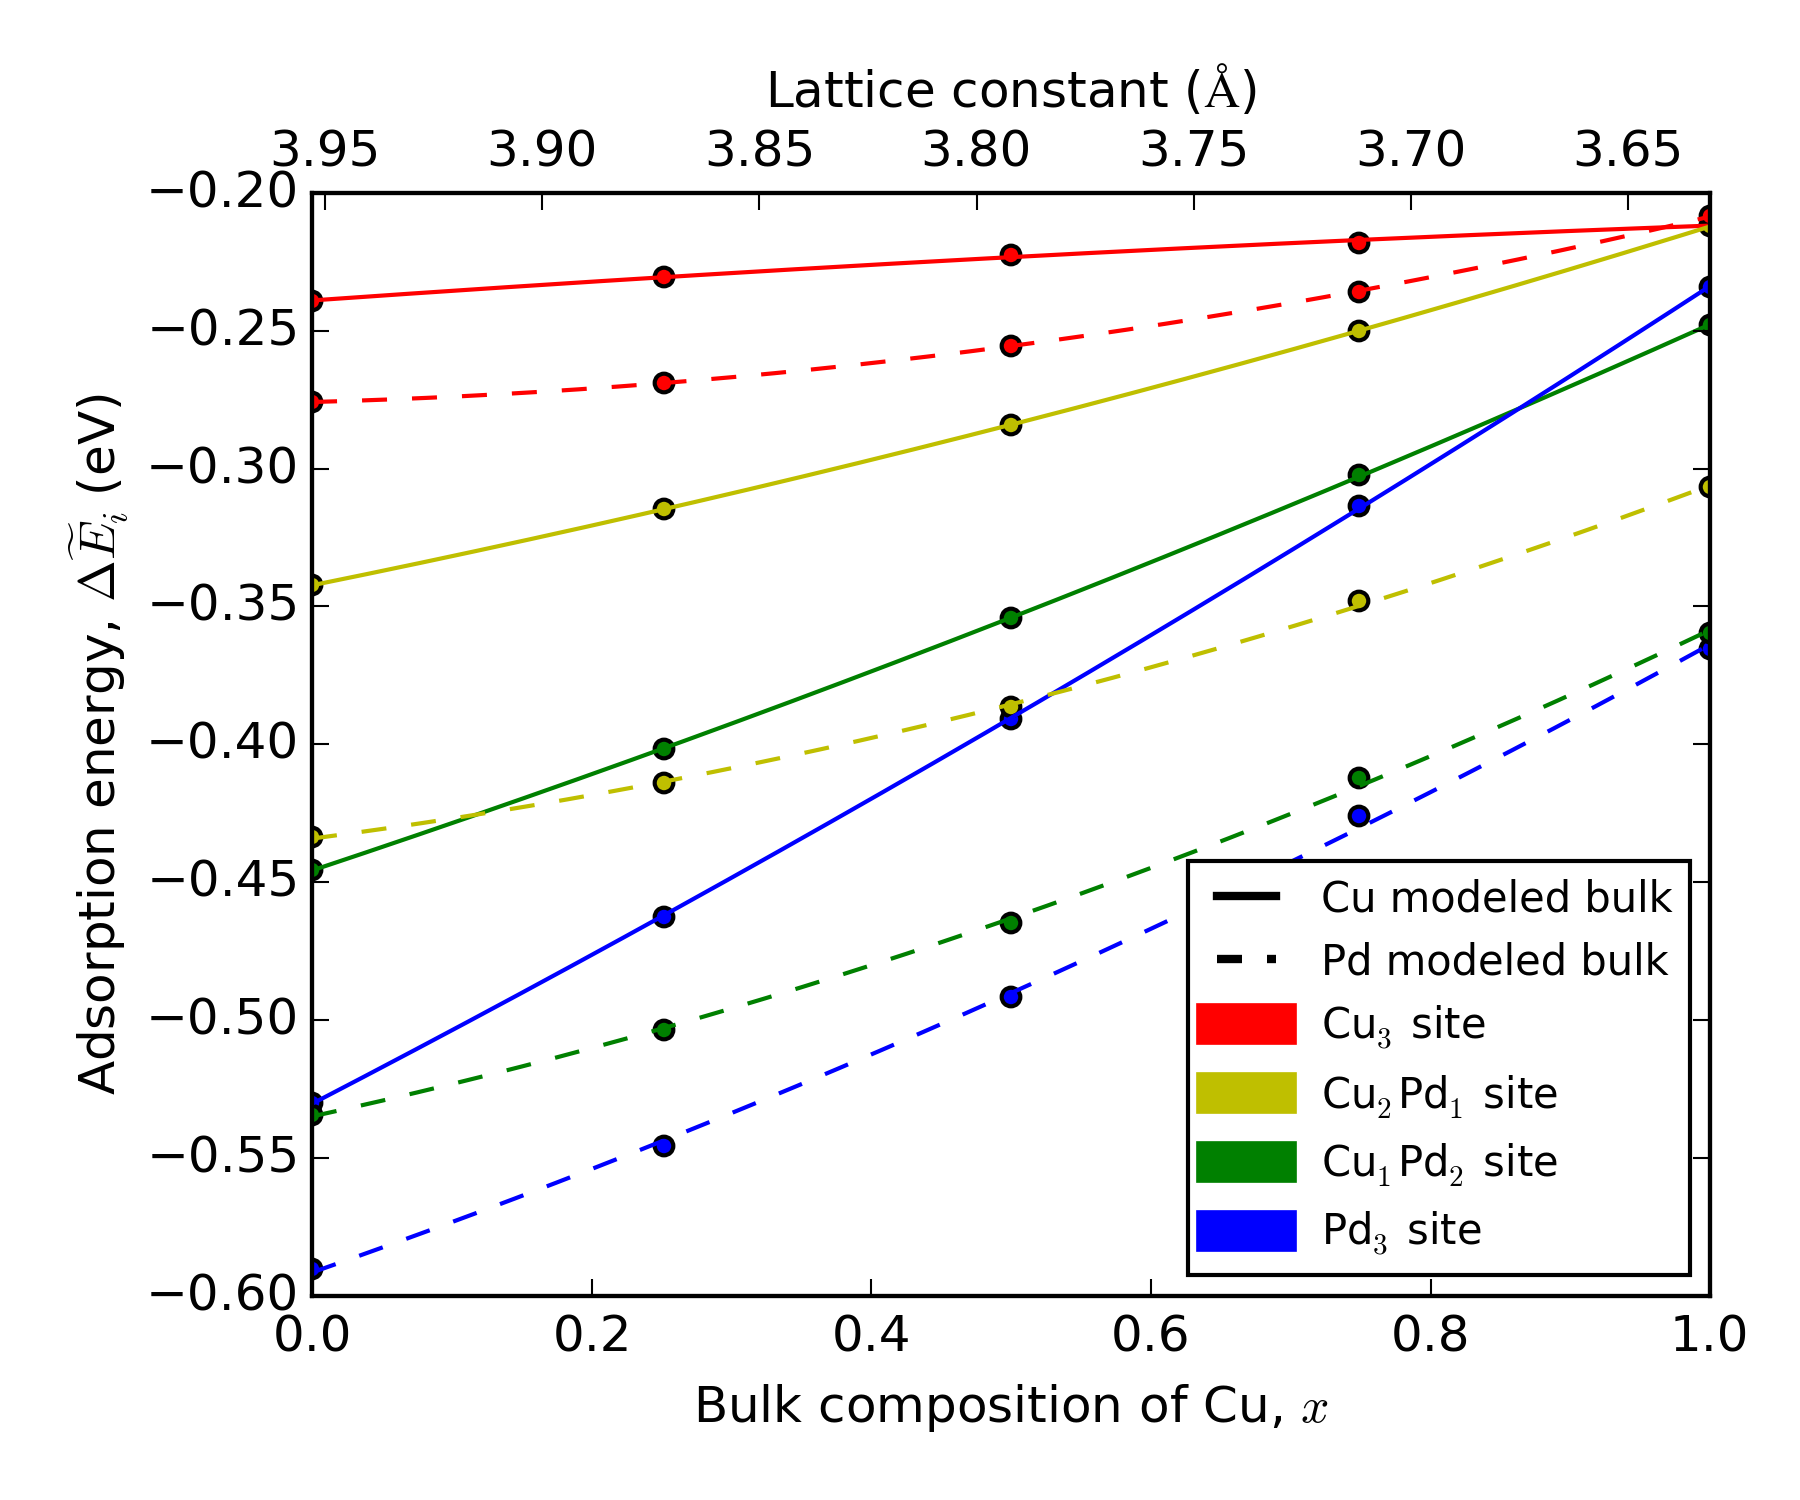
\includegraphics[width=5.5in]{./images/adsnrg.png}
\caption{Adsorption energies for a H atom plotted against lattice constant and bulk composition. Solid lines represent models with Cu atoms in the sub-surface layers while dashed lines represent Pd sub-surface atoms. Each color represents one of the surface configurations shown in Figure \ref{fig-configs}. \label{fig:ads-site}}
\end{figure}

Solid lines represent active sites embedded in a Cu slab, while dashed lines represent sites in Pd. There is a notable difference between the energies of the two data sets, with more favorable adsorption for sites embedded in Pd. This difference is characteristic of the ligand effects and puts some bounds on the possible variations with composition. This effect is typically small (\(< \; 0.05\) eV) and results in a slight shift of adsorption energies across lattice constants, leaving the trends relatively unchanged. The results can be converted from a basis of lattice constant to bulk composition using Equation \eqref{eqn-alpha} which is represented in the secondary \$x\$-axis of Figure \ref{fig:ads-site}.

\subsection{Active site probabilities and effective adsorption}
\label{sec:orgf7350e3}
To determine the effective adsorption energy, we need the active site distribution. The probability of finding each of the four active sites is determined by the surface composition and its ordering. The CuPd system forms a disordered fcc bulk alloy, so we assume that the surface is also randomly ordered. These distributions can also be determined computationally, using Monte Carlo techniques described in Chapter \ref{sec:ch6}. This means that the probability of finding a site is dictated by the composition of the site. Figure \ref{fig-rnd} shows this random distribution profile for the CuPd system as a function of surface composition. Similar statistical distributions have been calculated and compared to experimental observations for PdRu systems \cite{hartmann-2009-surfac-pdru}. For PdRu, an increased concentration of pure component metal active sites are observed over mixed component sites. Deviations from the distributions shown in Figure \ref{fig-rnd} are the result of short-range ordering on the surface. This short range ordering can also be accurately determined from simulation using the methods outlined in Chapter \ref{sec:ch6}.

\begin{figure}[h]
\centering
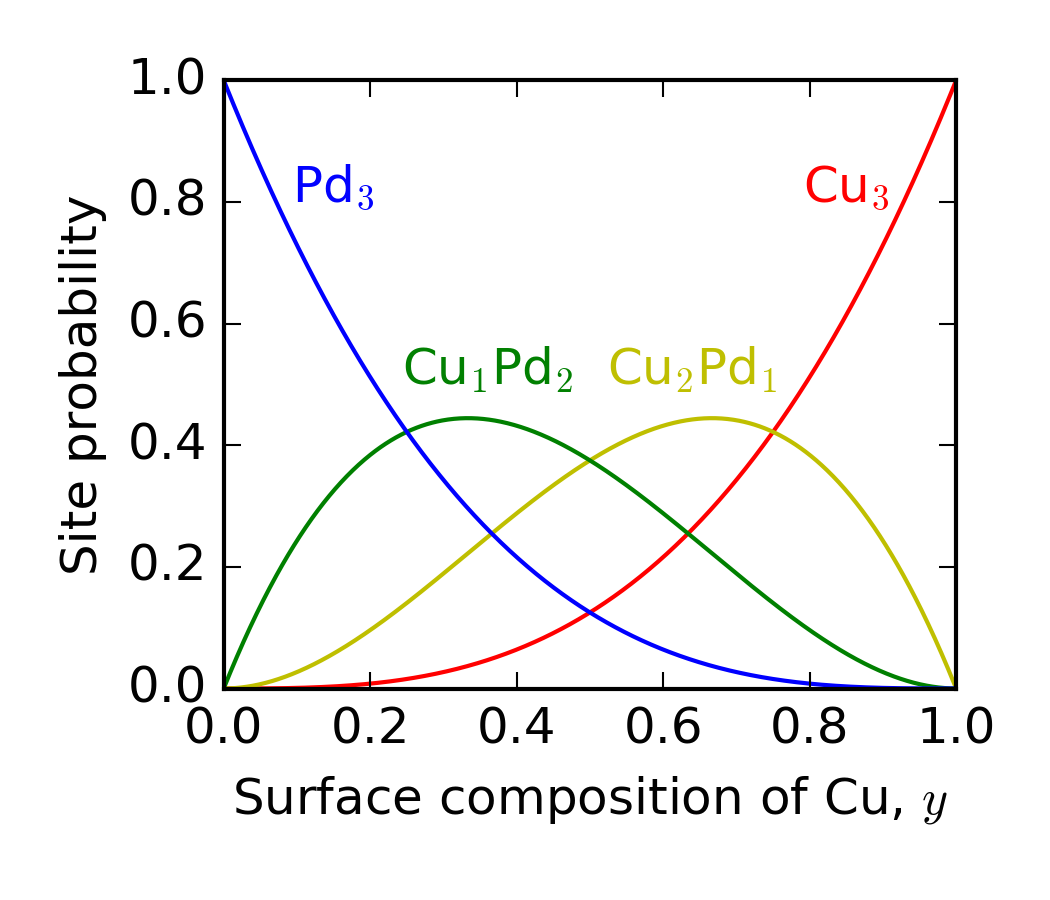
\includegraphics[width=3.5in]{./images/rndprob.png}
\caption{The fraction of active sites present on the clean surface of a CuPd alloy assuming a perfectly random distribution of surface atoms. \label{fig-rnd}}
\end{figure}

These distributions are based on arbitrary \emph{surface} compositions and do not account for segregation effects. Since there are three possible configurations of the mixed composition sites, it becomes three times more likely to find them. Weighting the adsorption energies determined using Equation \eqref{eqn:poly-ads}, with the probabilities described above, results in the effective adsorption energy (\(\Delta \widetilde{E}\)) shown in Equation \eqref{eqn-effective}.

\begin{eqnarray}
\Delta \widetilde{E}(x,y) = \sum\limits_i R_{i} Pr_{i}(y) \Delta E_{i}(x)
\label{eqn-effective}
\end{eqnarray}

where \(R_{i}\) is the number of configurations identical to configuration \(i\), \(Pr_{i}\) is the probability of slab configuration \(i\), and \(y\) is the surface composition of Cu. In the absence of segregation \(y \approx x\) and this equation becomes a descriptor of the observed adsorption energy on the surface as a function of the bulk composition of the alloy. However, segregation will only be negligible for systems with similar parent metals and adsorbates which do not interact strongly with the surface. Since most systems of interest do not fit these criteria we next develop a means of estimating the surface composition under reaction conditions.

\subsection{Estimating surface composition under reaction conditions}
\label{sec:org60b1346}
Segregation is a phenomena that reduces the surface free energy of alloys. In vacuum, it is generally observed that the less reactive metal of an alloy segregates to the surface \cite{ruban-1999-surfac-segreg,ruban-2007-theor-inves}. The Langmuir-McLean formulation of the Gibbs free isotherm (Equation \eqref{eqn-LM}) relates the surface and bulk compositions of a binary alloy to the Gibbs free energy of segregation \cite{miller-2008-surfac-segreg}.

\begin{eqnarray}
\frac{y}{1-y} = \frac{x}{1-x} \exp\left(\frac{-\Delta G^{seg}}{k_{B}T}\right)
\label{eqn-LM}
\end{eqnarray}

Figure \ref{fig:exp-seg} shows the segregation profiles resulting from Equation \eqref{eqn-LM} at 800 and 900 K using the experimental segregation energies \cite{priyadarshini-2011-high-throug}. The data shown in this figure was collected using low energy ion scattering spectroscopy (LEISS) which samples only the top layer concentration of an alloy with a predetermined bulk composition. Figure \ref{fig:exp-seg} shows that under ultra-high vacuum conditions the concentration of Cu at the topmost layer of the CuPd alloy will always be greater than the concentration in the bulk. This segregation is shown to increase as temperature drops until it reaches \(\approx 700\) K, below which the surface may not be at equilibrium with the bulk due to slow diffusion of metal atoms \cite{miller-2008-surfac-segreg}.

\begin{figure}[h]
\centering
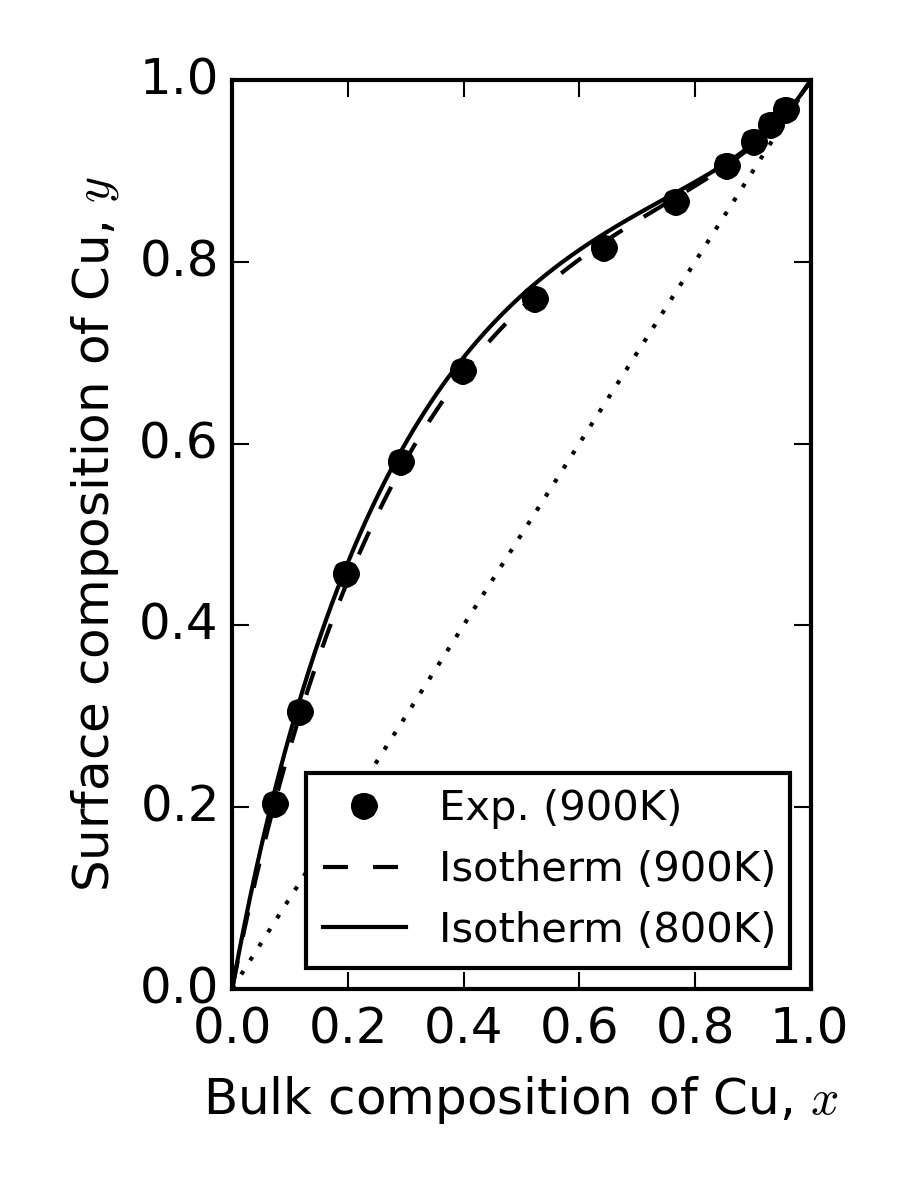
\includegraphics[width=3.5in]{./images/segvac.png}
\caption{Experimental surface segregation for CuPd alloy under ultra-high-vacuum conditions. Black dots represent experimental measurements of top surface layer concentrations at 900 K using LEISS. The dashed line shows the Gibbs isotherm fit to the experimental data at 900 K using the segregation energies found in Ref. \citenum{priyadarshini-2011-high-throug}. The solid line shows the Gibbs isotherm using the same segregation energies at 800 K. \label{fig:exp-seg}}
\end{figure}

In the presence of adsorbates, however, a strong adsorption bond to a more reactive metal may lead to segregation reversal. Both the vacuum and adsorbate-induced segregation can be lumped into a total Gibbs free energy of segregation under reaction conditions (Equation \eqref{eqn-balance}) \cite{kitchin-2008-alloy,miller-2008-effec-adsor}. The relevant segregation driving force for adsorption induced segregation is the difference in adsorption energy between the pure component metals. If adsorption is more favorable at one metal than the other it provides a driving force for segregation. We approximate this driving force as the difference in adsorption energy on Cu(111) and Pd(111), times the coverage of adsorbates.

\begin{eqnarray}
\Delta \widetilde{G} (x,y) = \Delta G^{seg}_{vac} (x,y) + \theta_{H} (x,y) \left(\Delta E^{Cu}_{ads} - \Delta E^{Pd}_{ads}\right)
\label{eqn-balance}
\end{eqnarray}

\noindent
where \(\Delta \widetilde{G}\) is the total Gibbs free energy of segregation, \(\Delta G^{seg}_{vac}\) is the Gibbs free energy of segregation in vacuum, \(\Delta E^{M}_{ads}\) is the adsorption energy of pure metal \(M\), and \(\theta_{H}\) is the coverage of hydrogen atoms on the surface. \(\Delta G^{seg}_{vac}\) is known from Figure \ref{fig:exp-seg}.  Under vacuum conditions or above the desorption temperature, \(\theta_{H}\) goes to zero and \(\Delta G^{seg}_{vac}\) is recovered as the total segregation energy. Likewise, if the adsorption energy difference between the two metals goes to zero. It is important to note that this is the simplest possible formulation for the adsorbate-induced contribution the segregation energy. It does not account for strain effects of the differences of pure active sites at difference alloy bulk compositions, which have been discussed in other work \cite{roudgar-2005-hydrog}. This results in an over prediction of favorable adsorption onto the surface. A more detailed discussion of the incorporation of strain effects can be found in the SI file of the published work \cite{boes-2015-estim-bulk}.

We solve for \(\theta_{\text{H}}\) using a simple Langmuir isotherm for dissociative adsorption of hydrogen onto the surface of the alloy \cite{miller-2012-segreg-at}. The isotherm is dependent upon adsorption energy for each individual adsorption site. These are estimated as a function of bulk composition as shown previously in Figure \ref{fig-configs}. Here, it is assumed that the dissociative adsorption energy on each site is independent of coverage. The coverage on an individual site \(i\) can then be expressed as shown in Equation \eqref{eqn-theta-site}.

\begin{eqnarray}
\theta_{i} (x) = \frac{\sqrt{\exp\left(\frac{-\Delta E_{i}(x)}{k_{B} T}\right) P_{H_2}}}{1 + \sqrt{\exp\left(\frac{-\Delta E_{i}(x)}{k_{B} T}\right) P_{H_2}}}
\label{eqn-theta-site}
\end{eqnarray}

\noindent
where \(\theta_{i}\) is the hydrogen coverage contribution from site \(i\), and \(P_{H_2}\) is the pressure of hydrogen gas. The total coverage of hydrogen on the surface of the alloy can then be obtained by summing the coverage on each site multiplied by the site probability, i.e. \(\theta_{H} (x,y) = \sum\limits_i R_{i} Pr_{i}(y) \theta_{i} (x)\). The total segregation energy can then be reformulated as a function of the bulk and surface composition of the alloy as shown in Equation \eqref{eqn-balance2}.

\begin{eqnarray}
\Delta \widetilde{G} (x,y) &=& -k_{B}T \ln\left(\frac{y(1-x)}{x(1-y)}\right) \nonumber\\
 &=&  \Delta H^{seg}_{vac} (x) - T \Delta S^{seg}_{vac} (x) \\
 & & + \theta_{H} (x,y) \left(\Delta \widetilde{E}(1,1) - \Delta \widetilde{E}(0,0)\right) \nonumber
\label{eqn-balance2}
\end{eqnarray}

Inserting Equation \eqref{eqn-balance2} into Equation \eqref{eqn-LM} leads to a single equation with a single unknown: the surface composition. This function then depends only on the bulk composition, the reaction conditions, the adsorption energies on each site, and the site distribution. We assume the adsorption energies are independent of coverage. At higher coverages than 0.25 ML, the adsorption energies may increase (become less stable) by up to 0.05 - 0.1 eV depending on the metal. Figure \ref{fig-seg} shows the predicted surface composition under reaction conditions for the CuPd system which results from the solution to Equation \eqref{eqn-balance2}. The segregation profiles shown represent the adsorbate-induced surface composition of the alloy. We performed the analysis for sites embedded in a Cu slab (solid) and Pd slab (dashed). The difference between the two profiles places bounds on our estimates.

\begin{figure}[h]
\centering
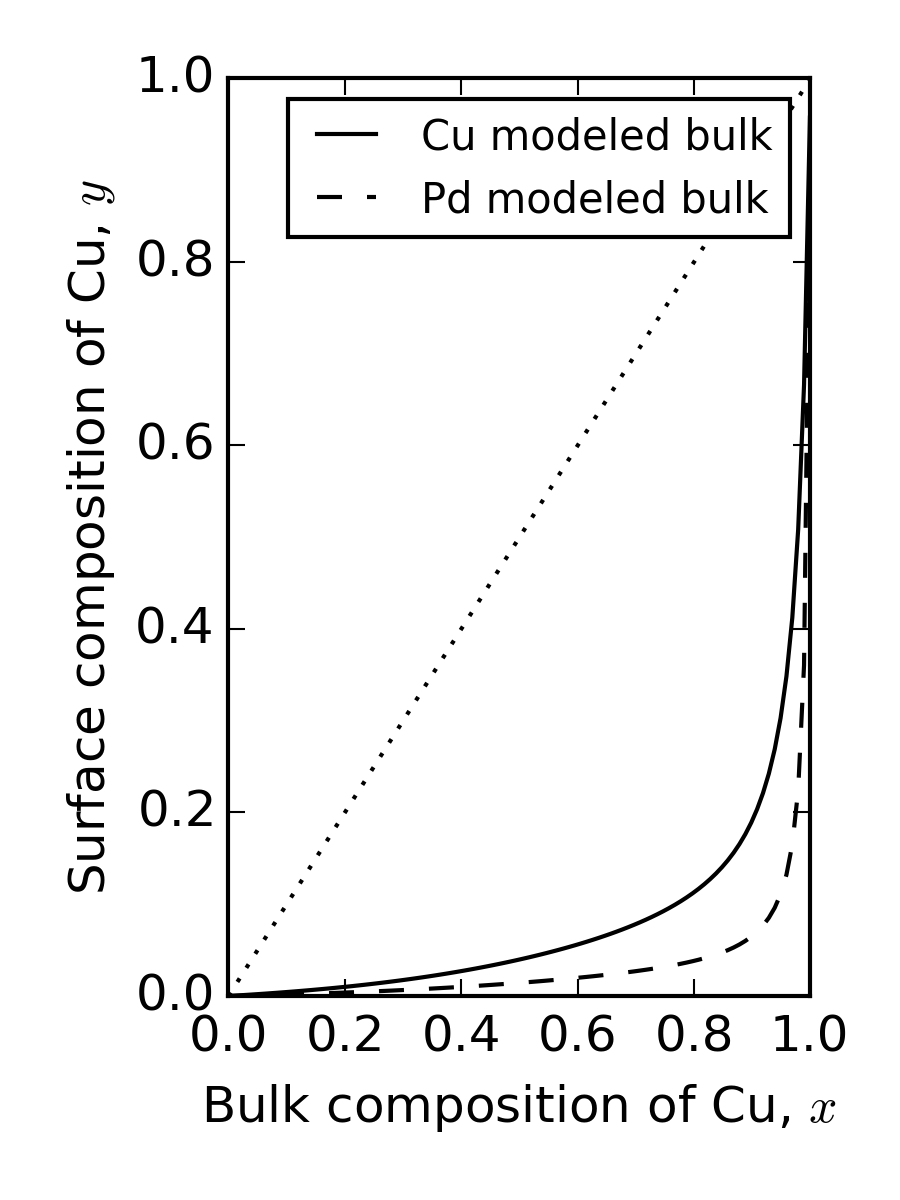
\includegraphics[width=3.5in]{./images/segtot.png}
\caption{Segregation profile of the CuPd system at 800 K and 1 atm of hydrogen. The solid line represents the predicted surface concentrations for active sites modeled on Cu sub-surface layers and the dashed line for Pd sub-surface layers. \label{fig-seg}}
\end{figure}

Comparison of Figures \ref{fig:exp-seg} and \ref{fig-seg} clearly indicates that the surface composition under reaction conditions is markedly different than in vacuum. This is a result of preferential bonding between hydrogen and adsorption site configurations which contain high concentrations of Pd, resulting in a substantial increase of Pd at the surface \emph{under reaction conditions}.

The effective hydrogen adsorption energies that are consistent with segregation for the CuPd systems and a comparison to the experimental results are included in Figure \ref{fig-results}. The solid blue line represents the effective adsorption energies predicted for the four surface configurations embedded in a Cu slab and the dashed line for the sites embedded in a Pd slab. Both sets of data show similar trends, with weaker adsorption energies on Cu-rich surfaces than on Pd-rich surfaces. The sites embedded in the Pd slab are more consistent with the experimental results, indicating that Pd-ligand effects are probably significant in determining the actual site reactivities.

\begin{figure}[h]
\centering
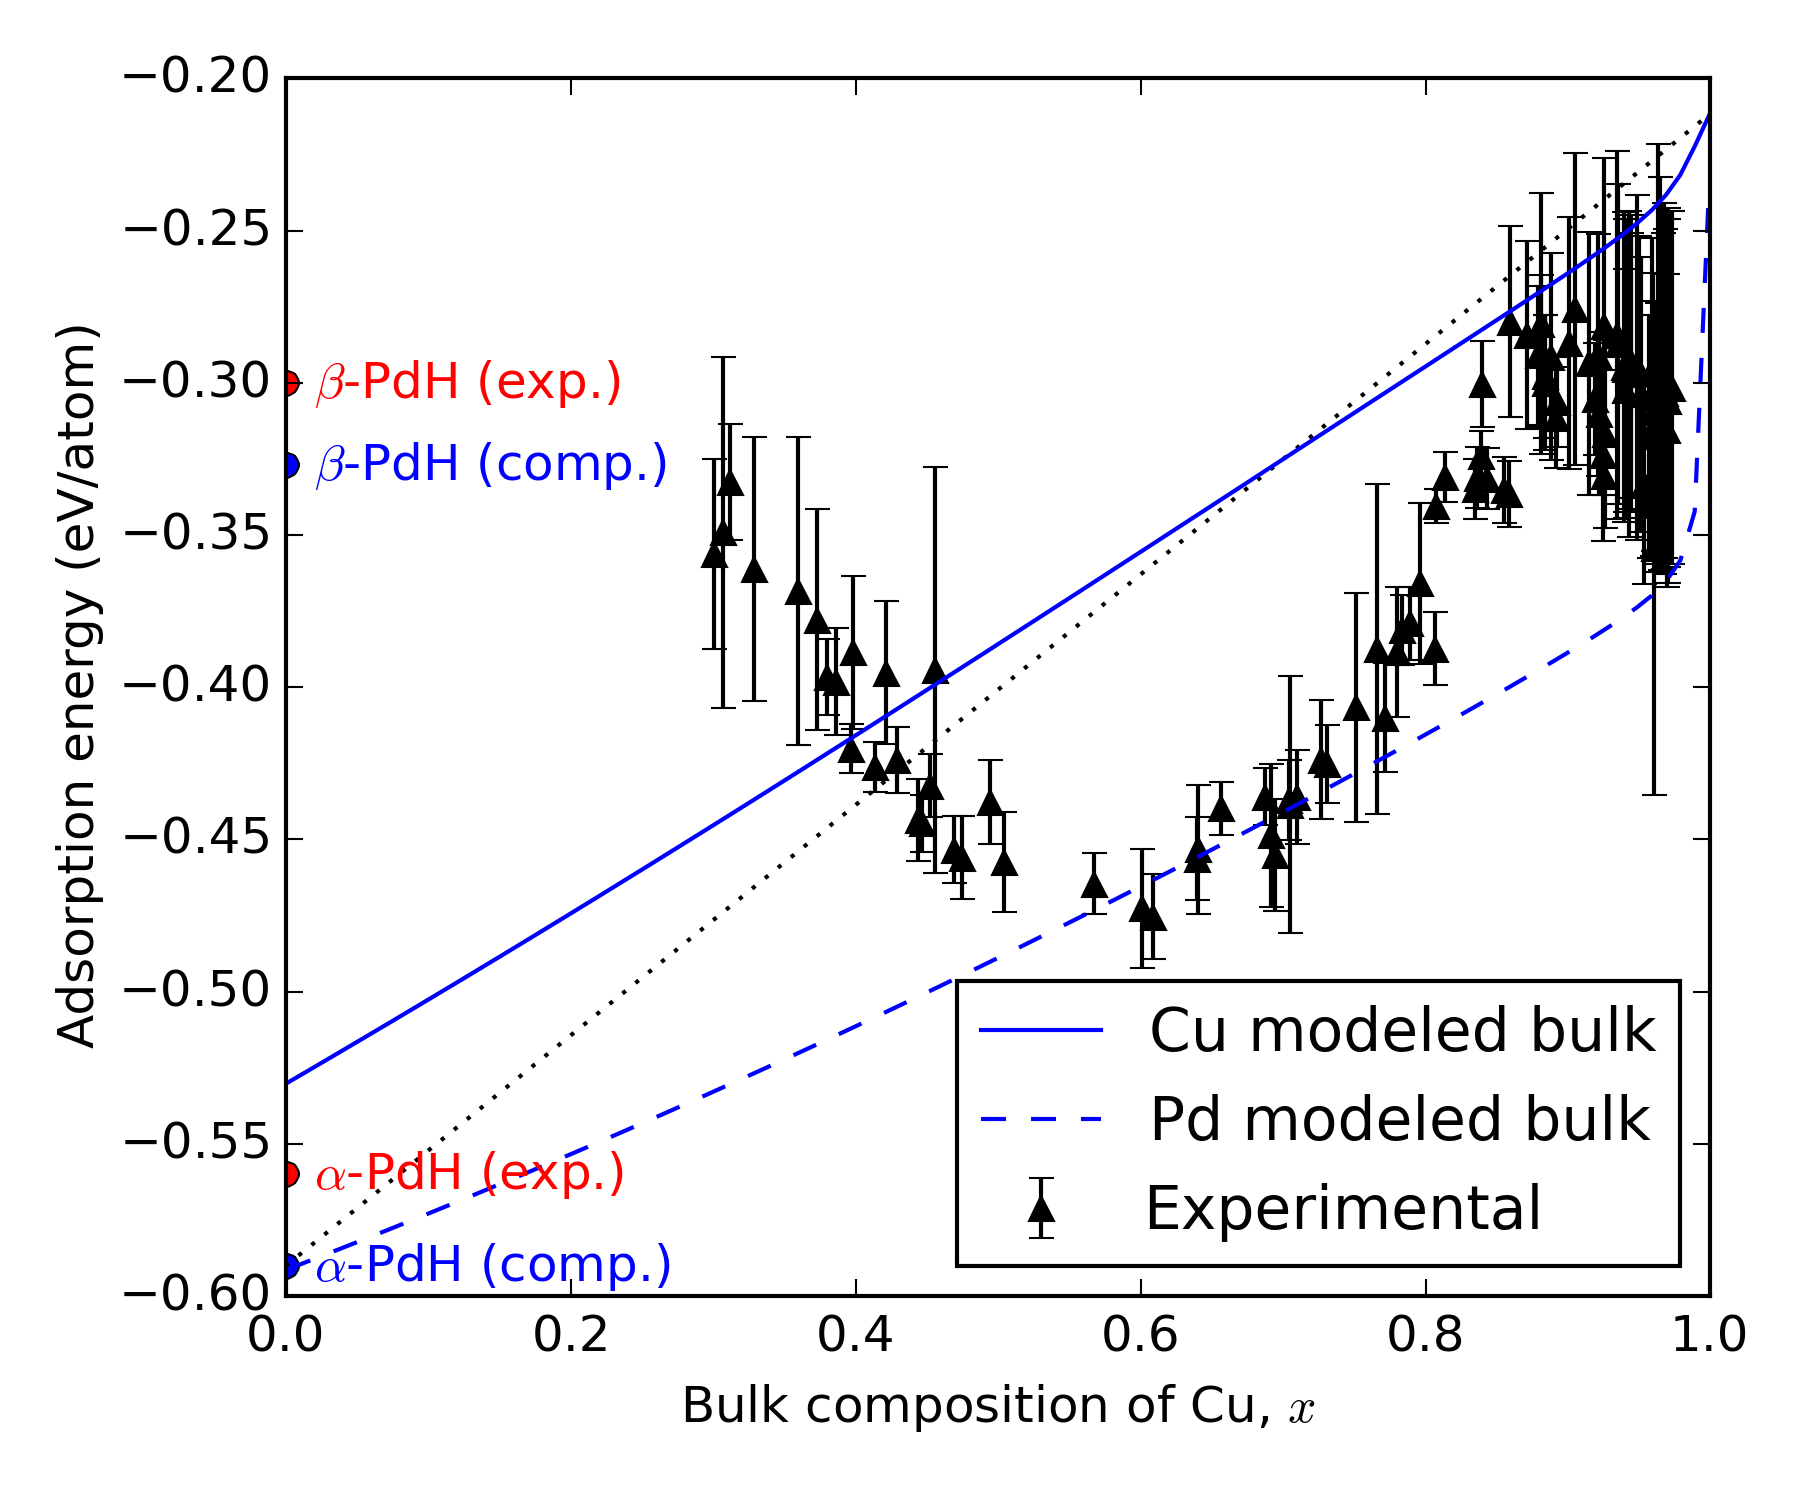
\includegraphics[width=5.5in]{./images/results.png}
\caption{Effective hydrogen adsorption energies on Cu\(_x\)Pd\(_{\text{1-}x}\) alloys modeled using adsorption site configurations embedded in bulk Cu (solid line) and Pd (dashed line) as a function of bulk alloy composition for an fcc(111) surface. The dotted black line represents a linear trend between adsorption energies of pure component metals. Black triangles represent experimental data shown in Figure \ref{fig:exp-ads} with corresponding experimental uncertainty. The experimentally determined adsorption energies for the \(\alpha\)- and \(\beta\)-Pd hydride phases are also shown in red. \label{fig-results}}
\end{figure}

The dotted black line represents the linear average between the adsorption energies of the pure component metals. From Figure \ref{fig-results} it can be seen that the experimental data is not well characterized by the adsorption energy of a single active site (a horizontal line) or the linear interpolation between the adsorption energy of the pure component metals. This is characteristic of segregation effects on the surface of the alloy, resulting in more favorable active sites at the surface under reaction conditions. This is supported by the fact that the effective adsorption calculated without segregation effects does not accurately predict the experimental adsorption trend either. Effective adsorption energy predictions without segregation effects can be found in the SI file of the published work \cite{boes-2015-estim-bulk}.

Predicted and experimental composition dependent adsorption energies are in good agreement for \(x > 0.5\). The deviation of experimental data away from the bounded region at \(x < 0.4\) is possibly due to the formation of a dense hydride phase which has different reactivity than the metallic surfaces modeled in this work. There are two PdH phases: the \(\alpha\)-phase, which has a very low H concentration, and \(\beta\)-phase, which forms a rock salt structure \cite{manchester-1994-h-pd}. Due to the low concentration of H in the \(\alpha\)-phase it is expected that the hydrogen adsorption energy will be quite similar to that on a pure Pd fcc configuration, such as the one incorporated in our model. The experimentally measured adsorption energy for the \(\alpha\)-PdH phase is -0.56 eV/atom \cite{obrien-2011-kinet-h}, which falls well within the predicted bounds of effective adsorption using our method as shown in Figure \ref{fig-results}. The experimental adsorption energy for the \(\beta\)-PdH phase was measured at -0.3 eV/atom \cite{obrien-2011-kinet-h}. Calculations were performed on both the fcc and hcp active sites of a Pd terminated stoichiometrically-equivalent \(\beta\)-PdH. The adsorption energies were determined to be -0.327 and -0.283 eV/atom for the hcp and fcc active sites, respectively. The energy for the more favorable hcp site is in good agreement with the experimental result of -0.3 eV/atom. The observed trend in experimental adsorption energies on the CuPd CSAF appear to be moving towards this higher energy, suggesting the formation of the \(\beta\)-hydride phase.

\section{Conclusions}
\label{sec:org978dae3}
In this chapter, we have shown that the reactivity of a CuPd alloy for H\(_{\text{2}}\)-D\(_{\text{2}}\) exchange cannot be explained simply by a single site, nor as a simple linear average of the pure metal components. The reactivity is determined by the distribution of active sites, which depends on the surface composition. The surface composition, in turn, depends on the bulk composition \emph{and} the reaction conditions as described in Chapter \ref{sec:ch1}.

We developed a methodology to estimate the reactivity of an alloy surface that takes these factors into account. We began by utilizing a basis set of active sites which spans the properties of the surface. Using DFT, we estimated the reactivity of each site by embedding the sites in metal slabs with geometric properties similar to a bulk alloy. Site distributions as a function of an arbitrary surface composition were estimated statistically. Finally, we solve for the surface composition by balancing vacuum and adsorbate induced segregation energies through the Langmuir-McLean formulation of the Gibbs isotherm.

Using this methodology, we estimated the dissociative adsorption energy of hydrogen on CuPd surfaces as a function of bulk composition. In parallel, we measured the adsorption energy of hydrogen on a composition spread alloy film.  This method was found to give good agreement with experimental adsorption energies for the CuPd system in the Cu rich region, falling within predicted bounds of \(\approx 0.08\) eV range at \(x > 0.5\). Below this range, there is poor agreement with experimental results which is possibly due to the formation of a hydrogen rich \(\beta\)-PdH phase.

\chapter{Atomistic Potentials: Atoms in, Energies out}
\label{sec:ch3}
In the previous chapter, we have demonstrated a high-level approach to characterizing the adsorption energy of a reaction on an alloy surface. Although useful as a screening tool, the results of this type of high-level study are not extremely precises, due to the course-graining built in. To provide more accurate representation of the inputs to this scheme, more accurate methods for lower time-scale studies are required.

In the following chapters we will discuss how some of these inputs can be achieved with improved accuracy using new atomistic potentials. Atomistic potentials approximate the PES for atomic systems by mapping potential energies and forces as functions of atomic positions. In this way, the energy of the system is retained, while the computational cost can be dramatically reduced. However, not all of these methods are equal in their speed or accuracy. The next three section describe the types of atomic potentials which will be discussed throughout the remainder of this dissertation; Namely, physical, cluster expansion, and machine learning potentials.

\section{Physical potentials}
\label{sec:org215ee65}
Physical potentials have been used for decades to capture the underlying physics of complex systems. They are parameterized to fit analytical expressions for the known physics of pairwise and many-body interactions. A common example, and one of the earliest physical potentials used to describe the pair-wise interaction is the Lennard-Jones potential \cite{jones-1924-deter-molec-field}. Classical force fields, such as CHARMM, UFF, and RESP \cite{brooks-1983-charm,rappe-1992-uff,casewit-1992-applic,cornell-1995-secon-gener,cornell-1996-secon-gener}, have slightly more sophisticated fitting forms, capable of capturing the chemistry more accurately than simply performing a summation over pair-wise interactions. The modified and standard embedded atom methods (MEAM and EAM) \cite{daw-1983-semiem-quant,baskes-1992-modif} are more accurate still, specifically for bulk systems. Finally, reactive force field (ReaxFF) \cite{duin-2001-reaxf} and the charge-optimized many-body (COMB) potentials \cite{liang-2012-variab-charg}, are apart of a general category of physical potentials designed to accurately represent the forming and breaking of chemical bonds.

All physical potentials are based on a long list of assumptions about the way the atoms in the system interact with one another. As such their parameters are almost always empirical in nature and typically set to experimentally relevant values. As additional parameters are included into the models, they necessarily become increasingly flexible; capable of fitting to more dynamic PESs. In general, this improves their accuracy, but this flexibility also comes with additional computational cost. This trade-off is demonstrated graphically in Figure \ref{fig-jacobs-ladder}.

\begin{figure}[h]
\centering
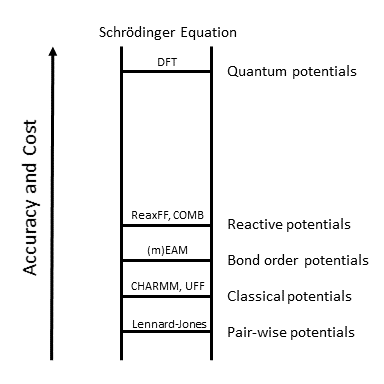
\includegraphics[width=4in]{./images/fig-jacobs-ladder.png}
\caption{A Jacob's ladder representation of the various levels of atomistic potentials. Physical potentials are listed in the ascending order of accuracy at the bottom of the later. Quantum potentials, derived from electronic interactions, are also included for context. \label{fig-jacobs-ladder}}
\end{figure}

Note that even though DFT and the Schrödinger equation are derived from electronic interaction, rather than atomic interaction, they follow the same trends. This concept of increased cost with accuracy follows a similar concept for choices of exchange-correlation functions in DFT known as ``Jacob's ladder'' \cite{perdew-2005-presc-desig}.

In this dissertation, we focus primarily on the reactive force fields since they provide the highest level of accuracy among all physical potentials. Bond order based reactive force fields, such as Tersoff \cite{tersoff-1988-new}, Brenner \cite{brenner-1990-empir}, and ReaxFF \cite{nielson-2005-devel-reaxf,duin-2001-reaxf} potentials, differ from classical force fields, such as UFF \cite{casewit-1992-applic,rappe-1992-uff}, CHARMM \cite{brooks-1983-charm}, or AMBER \cite{cornell-1995-secon-gener,cornell-1996-secon-gener}, which require that defined bonds remain fixed over the course of a simulation. ReaxFF potentials developed for Au and other metals normally employ three separate energy terms as seen in Equation \ref{eqn-base-reax}. \cite{jarvi-2008-devel-reaxf,keith-2010-react-forcef,cabrera-trujillo-2015-theor}

\begin{eqnarray}
E_{total} = E_{bond} + E_{over} + E_{vdw} \label{eqn-base-reax}
\end{eqnarray}

\(E_{bond}\) is for bond energies of atom pairs, \(E_{over}\) is an energy penalty to prevent overcoordination, and \(E_{vdw}\) accounts for van der Waals interactions and interatomic repulsions when interatomic distances are too small. ReaxFF potentials can also be parameterized to include 3-body terms which provide energy contributions from valence angles between sets of three Au atoms. Backman et al. developed a Tersoff potential for Au that involves 3-body terms \cite{backman-2012-bond}, but these terms are not always added to ReaxFF potentials for metals due to increased computational cost. The 3-body terms used in Chapter \ref{sec:ch4} have the same form as valence angle interactions in hydrocarbon ReaxFF potentials \cite{nielson-2005-devel-reaxf}.

\section{Cluster expansion potentials}
\label{sec:org351763e}
The cluster expansion \cite{sanchez-1984-gener-clust,shi-2007-first-princ,miller-2013-simul-temper} is another type of potential which is derived from empirical fitting. These models operate on a lattice structure where the nodes are held at fixed positions. The nodes of the lattice are typically the locations of atoms, and the occupancy of the node is designated by an integer spin variable. The spins indicate the element which occupies the node, or in the case of adsorbates, if the site is occupied by an adsorbate or not. The cluster expansion is comprised of a sum of spin-products of singlets, pairs, triplets, etc. over the lattice sites. By fitting to \emph{ab-initio} results of various enumerations of the lattice (\emph{i.e.} different combinations of the spins), the coefficients for each expansion function can be determined, and then used predictively for new spin configurations.

These techniques have proven effective for representing the kinetic properties of oxygen adsorption on Pd \cite{frey-2014-implic-cover}. Multiple cluster expansions can also be coupled to account for adsorption at multiple sites \cite{han-2005-surfac-segreg,chen-2011-order-oxygen}. However, due to the nature of their construction, cluster expansions are limited to Monte Carlo simulations of configurations in the ground state. Cluster expansions are also basically limited to the lattice type they were trained for; one cannot make predictions about a bcc alloy from an fcc cluster expansion.

\section{Machine learning potentials}
\label{sec:org1d1f3c0}
Another intriguing category is machine-learning potentials that ``learn'' the PES directly through a minimization of residuals with no \emph{a priori} knowledge of the underlying physics, e.g. Gaussian regression functions \cite{rasmussen-2004-gauss-proces} and artificial neural networks (NN) \cite{haykin-2009-neural-networ}. We refer to these as mathematical potentials because they are not influenced by any underlying physics.

These potentials are becoming more popular in chemical applications \cite{behler-2011-neural,behler-2014-repres}. Specifically, recent descriptive models from Behler and Parrinello \cite{behler-2007-gener-neural} have expanded the applications of neural networks to ``high-dimensional'' systems that can account for variable numbers of atoms, multiple compositions, and reactions involving thousands of atoms. Such networks have already been implemented on a large range of systems, including: Si bulk structures \cite{behler-2008-press}, water clusters \cite{morawietz-2013-densit-funct}, Cu surfaces \cite{artrith-2012-high}, ZnO \cite{artrith-2011-high}, and even a quaternary system of Cu/Au/H/O \cite{artrith-2015-grand-cu}. This opens the door for potentials to be developed that are accurate and transferable across diverse bulk, surface, and cluster regimes.

Specifically, Cartesian feed-forward neural networks (NN) have been in use for modeling PESs \cite{witkoskie-2005-neural-networ,behler-2007-repres-molec}. Although this technique is not specific to modeling PESs, it has proven to be well suited for this application \cite{blank-1995-neural-networ}. Their general framework consists of an input layer, one or more hidden layers each with multiple nodes, and an output layer. The connections between the nodes of the framework are individually weighted. These weights represent the fitting parameters of the NN. For modeling a PES, the input layers are the Cartesian-coordinates of a system with a fixed number of atoms. The nodes of the hidden layers are linear combinations of these coordinates with varying weights. Each layer is also multiplied by an activation function (which often has a bounded non-linear form) to allow the NN potential to fit to arbitrarily shaped PESs. Finally, the output layer has a single value which represents the energy for the given configuration of atoms (sometimes forces are output as well).

The flexible nature of these models makes them ideal candidates for simulations at longer time-scales, such as MC and MD applications. NNs are also capable of sampling any number of different configurations and can be trained to arbitrary accuracy \cite{hornik-1989-multil}. Despite these advantages, Cartesian feed-forward NNs are limited to systems of atoms of fixed composition and size. To create a Cartesian NN capable of simulating a different number of atoms, an entirely new NN must be trained. This includes performing all new \emph{ab-initio} calculations with the desired number of atoms to train the system to which makes this process too computationally demanding for larger systems and makes longer time-scale methods intractable.

Behler and Parrinello developed an approach which allows systems of atoms of arbitrary size to be fit to a feed-forward NN framework \cite{behler-2007-gener-neural}. To prevent the use of excessive feed-forward NNs, every local environment is designated a ``fingerprint'', made up of a reduced number of variables which are still descriptive for the system. With a sufficient number of symmetry functions, even systems with a larger number of atoms can be uniquely distinguished from one another. For example, a system of two gas-phase atoms in the ideal gas limit can be described by the six Cartesian-coordinates of the atoms, but in this simple case the single variable which represents the distance between the two atoms is sufficient to represent the entire PES. This way, only 1 feed-forward NN per type of element is needed. This approach makes a very diverse range of applications accessible to a single potential. It also creates an opportunity for combining a more diverse range of training sets which creates future possibilities for more chemically advanced applications.

Both \(G^{2}\) and \(G^{4}\) symmetry functions are implemented in the following chapters, as described in Ref. \citenum{behler-2011-atom,bartok-2015-gauss-approx-poten}. These symmetry functions were used to characterize each atom's local environment to a single variable. The expressions of \(G^{2}\) and \(G^{4}\) are given in Equations \ref{eq-G2} and \ref{eq-G4}, respectively.

\begin{eqnarray} \label{eq-G2}
G_{i}^{2} = \sum_{j}e^{-\eta(r_{ij} - r_{s})^2} f(r_{ij})
\end{eqnarray}

\begin{eqnarray} \label{eq-G4}
G_{i}^{4} = 2^{1-\zeta} \sum^{all}_{j,k \neq i} (1 + \gamma \cos\left(\theta_{ijk}\right))^{\zeta} e^{-\eta(r^{2}_{ij}+r_{ik}^2)} f(r_{ij}) f(r_{ik})
\end{eqnarray}

For all equations, \(r_{ij}\) is the distance between considered atom \(i\) and all other atoms \(j\). Parameters \(\eta\), \(\gamma\), and \(\zeta\) can be varied to produce unique outputs for various local atomic environments. \(G^{4}\) symmetry functions are meant to account for the angle between a system of three atoms. \(\theta_{ijk}\) is the angle between the three atoms and is defined as \(\theta_{ijk} = \arccos(r_{ij} \cdot r_{ik} / r_{ij} \cdot r_{ik})\). For further details on the theory behind Behler-Parrinello NNs, we refer to previous work \cite{behler-2007-gener-neural,behler-2011-atom}. Based on this formulation it becomes clear why these functions quickly become expensive for large systems of atoms. This is accounted for by the cutoff function \(f\) which is defined in Equation \ref{eq-cutoff}, which eliminates contributions from atoms outside a cutoff radius.

\begin{eqnarray} \label{eq-cutoff}
f(r_{ij}) =
\begin{cases}
\frac{1}{2} \left(\cos\left(\frac{\pi r_{ij}}{R}\right) +1\right) & \textrm{for} \; r_{ij} \leq R \\
0 & \textrm{for} \; r_{ij} \geq R \\
\end{cases}
\end{eqnarray}

The cutoff radius, \(R\), is applied to each atom in each image in the training set to keep the cost of the symmetry function small. Thus, the goal is to find a value of \(R\) that is large enough to capture meaningful atomic interactions but one that is not too large to result in high computational costs. These standard NN potentials are not suited for systems of atoms that have long-range interactions that extend outside the cutoff radii. In the absence of this cutoff radius, it has been proven that NNs are capable of arbitrary levels of accuracy \cite{hornik-1989-multil}. Also, such long-range interactions can be accounted for as shown for ZnO \cite{artrith-2011-high}. However, since long-range interactions are not expected in the metal systems presented in this dissertation, there is no need for incorporation of more sophisticated methods.

All NN training was performed using an iterative methodology outlined as follows. The process begins by defining some small subset of \emph{ab-initio} calculations to be added to the first training set. Ideally, these calculations are descriptive of the boundaries of the users search space in some way. Two different frameworks of NN were then trained to this subset of data. These two NN were then used to make energy predictions on configurations not included in the original training set. These additional calculations are frequently generated by MD trajectories using the existing NN, or an enumeration of the search space. Since each NN utilizes a different number of hidden layers and nodes, the energy predictions will differ. When the two NNs predict similar energies, it is likely that the structure represents a region of the PES which is well trained. Conversely, regions which require further training will be represented by structures with the largest difference in predicted energies. A certain portion of these poorly predicted structures can then be calculated using the previously selected \emph{ab-initio} technique and used to train the next iteration of NN frameworks. In this way, subsequent improvement of the NN can be obtained using the iterative approach depicted in Figure \ref{fig-training-process}.

\begin{figure}[h]
\centering
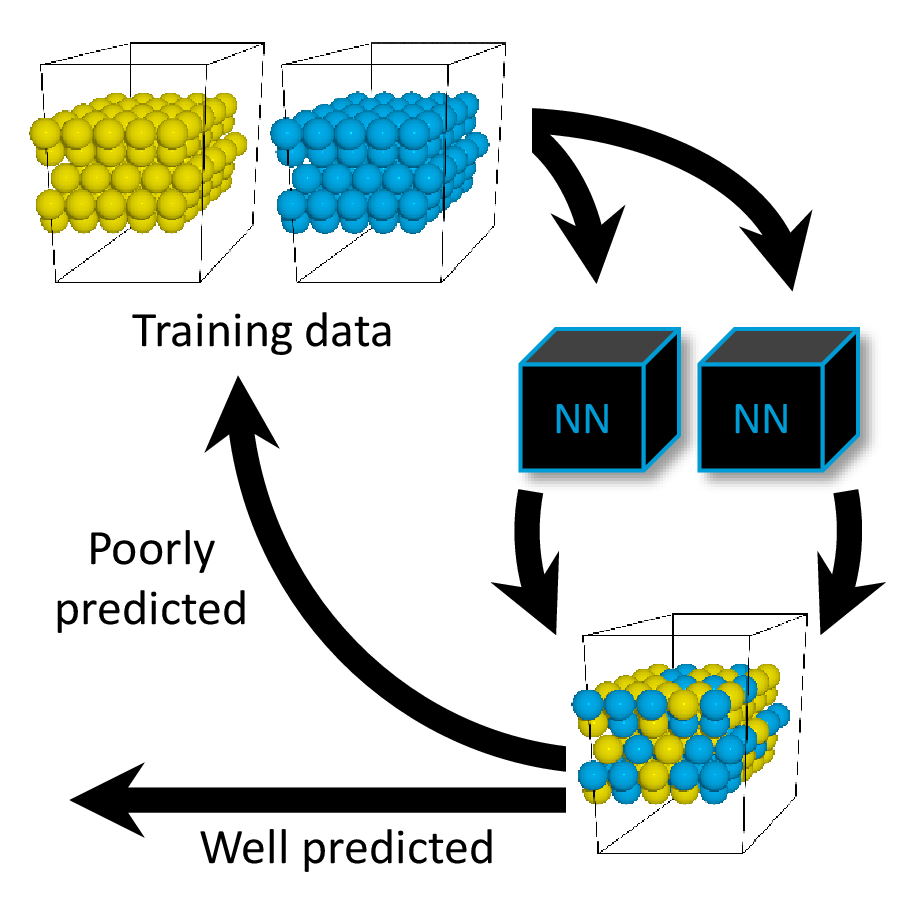
\includegraphics[width=3in]{./images/training-process.png}
\caption{\label{fig-training-process}
Diagram of the iterative training process. We begin with a sparse training set spanning the region of the PES we are interested in; this is generated from EMT in this work. We use multiple NNs to validate new images in the region of interest, adding structures to the trainings set which the NNs do not agree on. This process is repeated until the NN is sufficiently accurate.}
\end{figure}

Training of all NNs in this dissertation were performed using AMP \cite{khorshidi-2016-amp}, which is a code produced by the Peterson group at Brown University. This software provides a convenient interface with the Atomic Simulation Environment (ASE) software package \cite{bahn-2002-objec-orien}, further increasing the reusability and reproducibility of the methods and calculations performed in this dissertation. The NN calculator parameters for each chapter are included with the SI file of each published manuscript. These files include all of the variables needed to reproduce each NN as well, including symmetry functions, cutoff radii, and hidden layers and nodes.

\chapter{Neural Network and ReaxFF Comparison for Au Properties}
\label{sec:ch4}
\section{Introduction}
\label{sec:org965409f}
In this chapter, we compare the performance of a widely used physical potential, ReaxFF, with the more recently developed Behler-Parrinello NN potential. We have trained both to subsets of a full dataset comprised of \(\approx\) 10,000 DFT calculations. We chose Au for this study due to its diversity of known nanoscale structures. The fact that long-range electronic interactions are screened in Au makes it an appropriate system to model with atomistic physical and mathematical potentials that are less suited for long-range interactions such as ReaxFF and NNs. (We note that long range effects can be incorporated into Behler-Parrinello NN potentials, e.g. as has been done for ZnO \cite{artrith-2011-high}).

We have benchmarked both potentials to our quantum chemistry dataset that contains information from DFT bulk equation of state (EOS) data, vacancy formation energies, surface energies, adatom diffusion profiles, slipping barriers, and cluster binding energies. Parameterization of ReaxFF potentials were automated using the Monte Carlo Force Field optimization (MCFFopt) tool in ADF \cite{velde-2001-chemis-adf,iype-2013-param-monte}. Our NN was parameterized using the Atomistic Machine-learning Potentials (AMP) code from the Peterson group at Brown University  \cite{khorshidi-2016-amp}. This allows feed-forward neural networks to be developed inside the atomic simulation environment (ASE) \cite{bahn-2002-objec-orien}. All details of the trained NNs are stored in a JSON file which can be found in the supporting information (SI) file of the published work \cite{boes-2016-neural-networ}.

\section{Methods}
\label{sec:org69ec2b0}
\subsection{Density Functional Theory}
\label{sec:org2dd44ec}
In this chapter, \emph{k}-points were represented using Monkhorst-Pack grids \cite{monkhorst-1976-special-point} with a density of at least 14 \texttimes{} 14 \texttimes{} 14 for a single atom of Au in the primitive ground state configuration. Kohn-Sham orbitals were expanded up to energy cutoffs of at least 300 eV to attain an energy convergence of at least 5 meV/atom. All calculations involving relaxations were completed with relaxation criteria of \(< 0.05\) eV/\AA{}. Unless otherwise noted, transition states were determined using the climbing image nudged elastic band (NEB) method \cite{henkelman-2000}. The details for all the DFT calculations are included in an ASE database that is embedded in the SI file of the published work \cite{boes-2016-neural-networ}. Instructions on how to access this database and reproduce these calculations can also be found in the SI along with more details on the methods used in this chapter.

The full DFT training set contained 9,972 calculations that included 905 bulk, 1,022 surface, and 8,045 cluster configurations. The majority of these calculations (9,076 calculations) were taken from coordinate relaxation steps performed by VASP. These structures are the incremental steps taken from its initially guessed positions to the ground state configurations predicted by GGA-PBE. Each of the structures in a particular relaxation are very similar from one relaxation step to the next. The remaining 896 calculations are either the local ground state configurations or images from optimized NEB calculations. Our bulk Au data were obtained from the EOS data for a variety of bulk structures. Vacancy formation and diffusion calculations were also included in the bulk dataset. Our surface dataset includes calculations on fcc(111) surfaces as well as a variety of fcc(100) surface diffusion pathways that were originally generated in previous work by Pötting et al. \cite{potting-2010-self-diffus}. The training set used single-point energies on the latter coordinates (without geometry relaxations) calculated using the methods listed above. Our cluster data include various 3D ordered, planar, and disordered structures that contain up to 126 atoms.

\subsection{Reactive Force Field}
\label{sec:org5a6be0d}
We parameterized our Au ReaxFF using the MCFFopt tool implemented in ADF \cite{velde-2001-chemis-adf,iype-2013-param-monte}. MCFFopt seeks to minimize an objective function by randomly changing force field parameters within a predefined range. The Monte Carlo nature of this process allows some parameter changes that increase the objective function. This ``annealing'' allows the optimizer to sample a larger parameter space and potentially produce multiple distinct parameter sets. This approach can also find parameter sets with less total error than the traditional parabolic search parameter optimization \cite{iype-2013-param-monte}. Further information on running the MCFFopt procedure and optimized force field parameters are available in the SI file of the published work \cite{boes-2016-neural-networ}.

Au ReaxFF potentials appear to have an optimal training set size. Fitting to larger training sets does not always improve the quality of the ReaxFF potential, and this overfitting is found to bias predictions toward certain geometry types. As a result, the ReaxFF training set was constructed using the 848 ground state geometries from within the training set. Out of these geometries, the number of calculations classified as bulk, surface, and cluster structures are roughly equal. During ReaxFF parameterizations, each geometry in the training set is also assigned a weight depending on its relative importance in the overall fitting procedure. Our goal was to produce a ReaxFF potential with reasonable accuracy across these three different structure regimes, so most of the geometries were given a weight of one. In principle, one could increase weights to parts of the PES so that properties, such as desired lattice constants, bulk moduli, or barrier heights would be accurately reproduced. However, weighting a potential in this way will affect its ability to make accurate predictions in less-weighted regions of the PES.

Figure \ref{fig-reax-train} shows the error distribution of residual error between the trained ReaxFF and DFT training set data labeled by geometry type. Errors in bulk data greater than 0.2 eV stem from an unphysical convex region in the ReaxFF functional form which causes bulk EOS data to significantly deviate from the DFT data at atomic volumes ranging from 60-200 \AA{}\(^{\text{3}}\)/atom. Since these atomic volumes fall outside those found in most simulations involving bulk and surface structures of Au, these inaccuracies are not a cause for significant concern. However, large errors in bond energies for pairs of atoms at intermediate distances may be problematic for molecular clusters.

\begin{figure}[h]
\centering
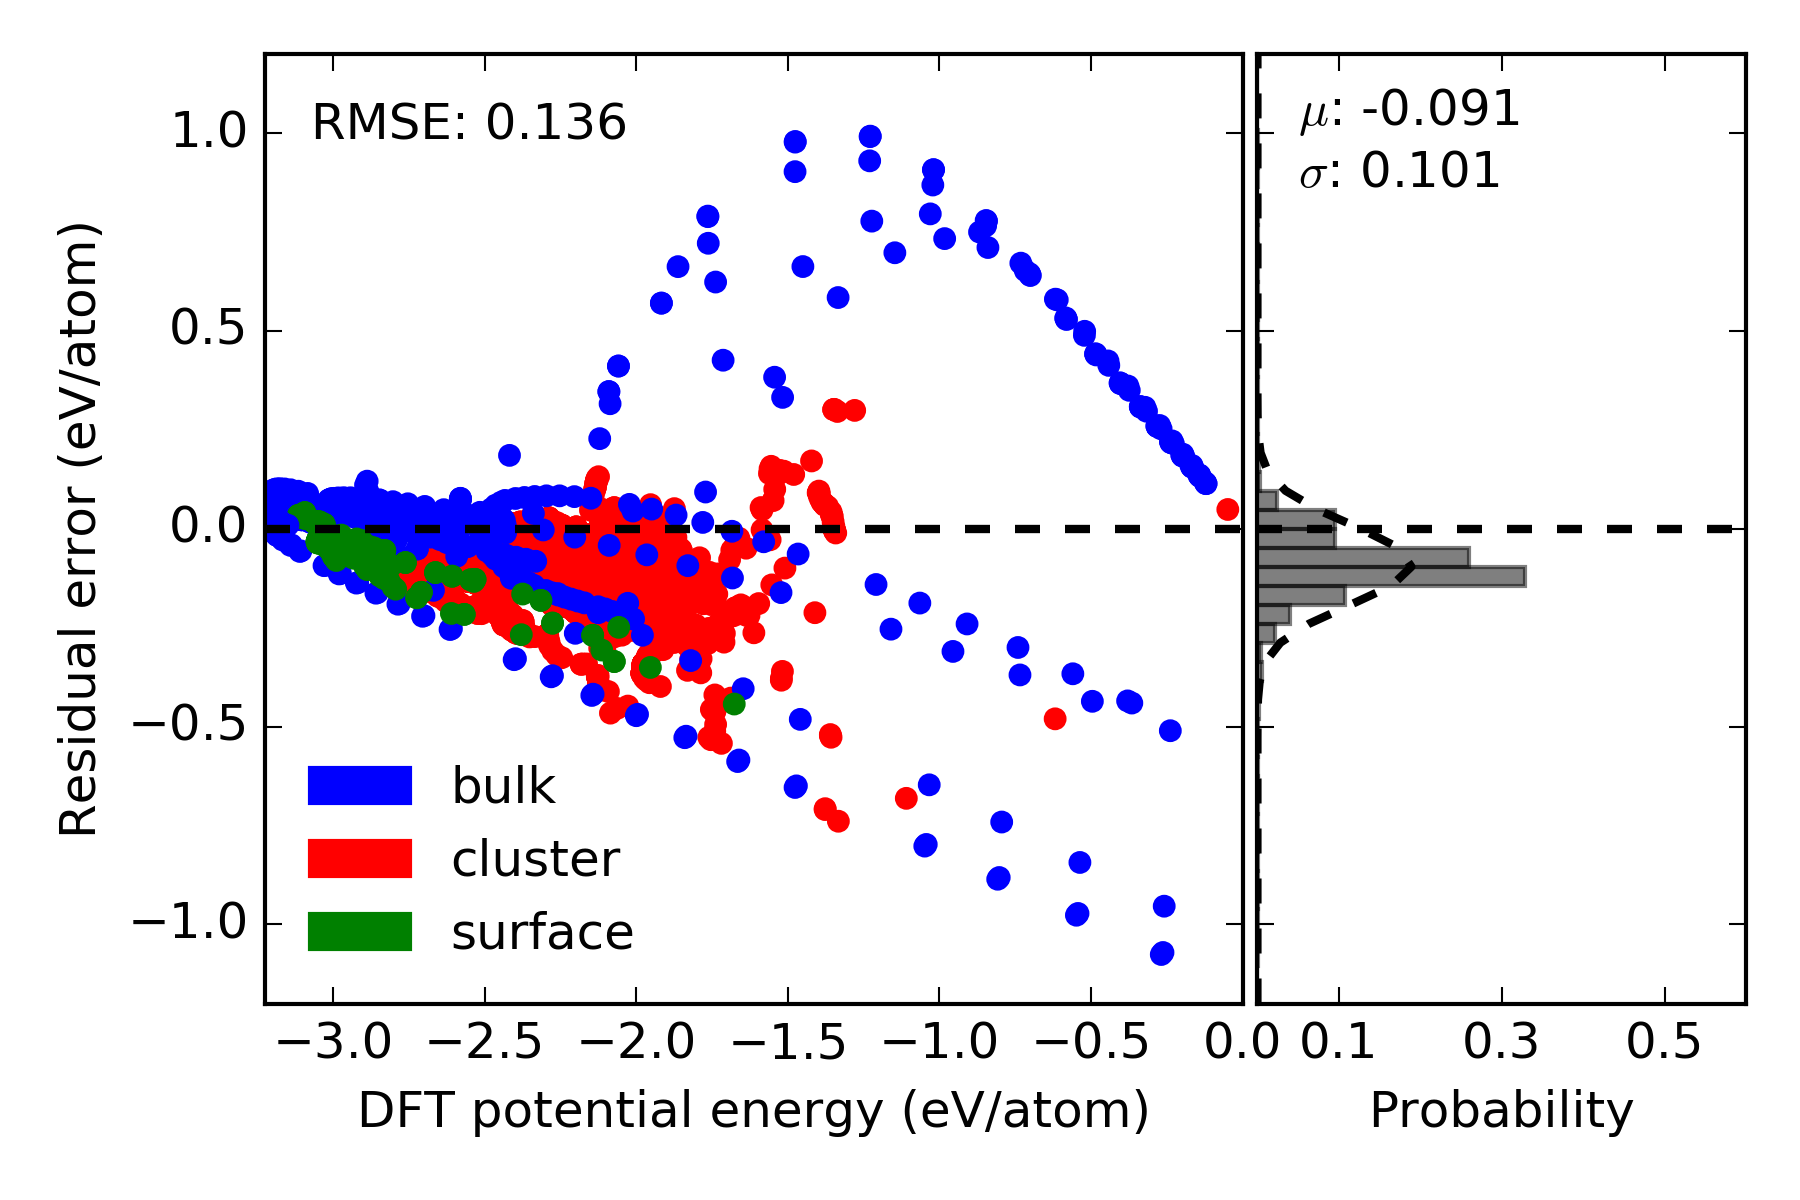
\includegraphics[width=5.5in]{./images/fig-reax-train.png}
\caption{\label{fig-reax-train}
Energy residual error to the training set data broken down by bulk, surface, and cluster geometries for the ReaxFF potential.}
\end{figure}

A predefined validation set consisting of 238 calculations (out of the total 9,972 DFT calculations) was set aside to test the transferability of predictions from our ReaxFF and NN potentials. This validation set was chosen to represent a variety of different Au structure types which are represented in the results section of this work. By reporting probability distributions for both the training and validation sets, we can determine the degree that our potentials show selection bias. For an ideal fitting procedure, the probability distributions for both the training and validation set would match, and any differences between the two would signify an over- or under-sampling. Figure \ref{fig-reax-valid} shows the residual error for the validation calculations labeled by geometry type. Significant deviations were found in bulk and cluster calculations from the validation and training set data.

\begin{figure}[h]
\centering
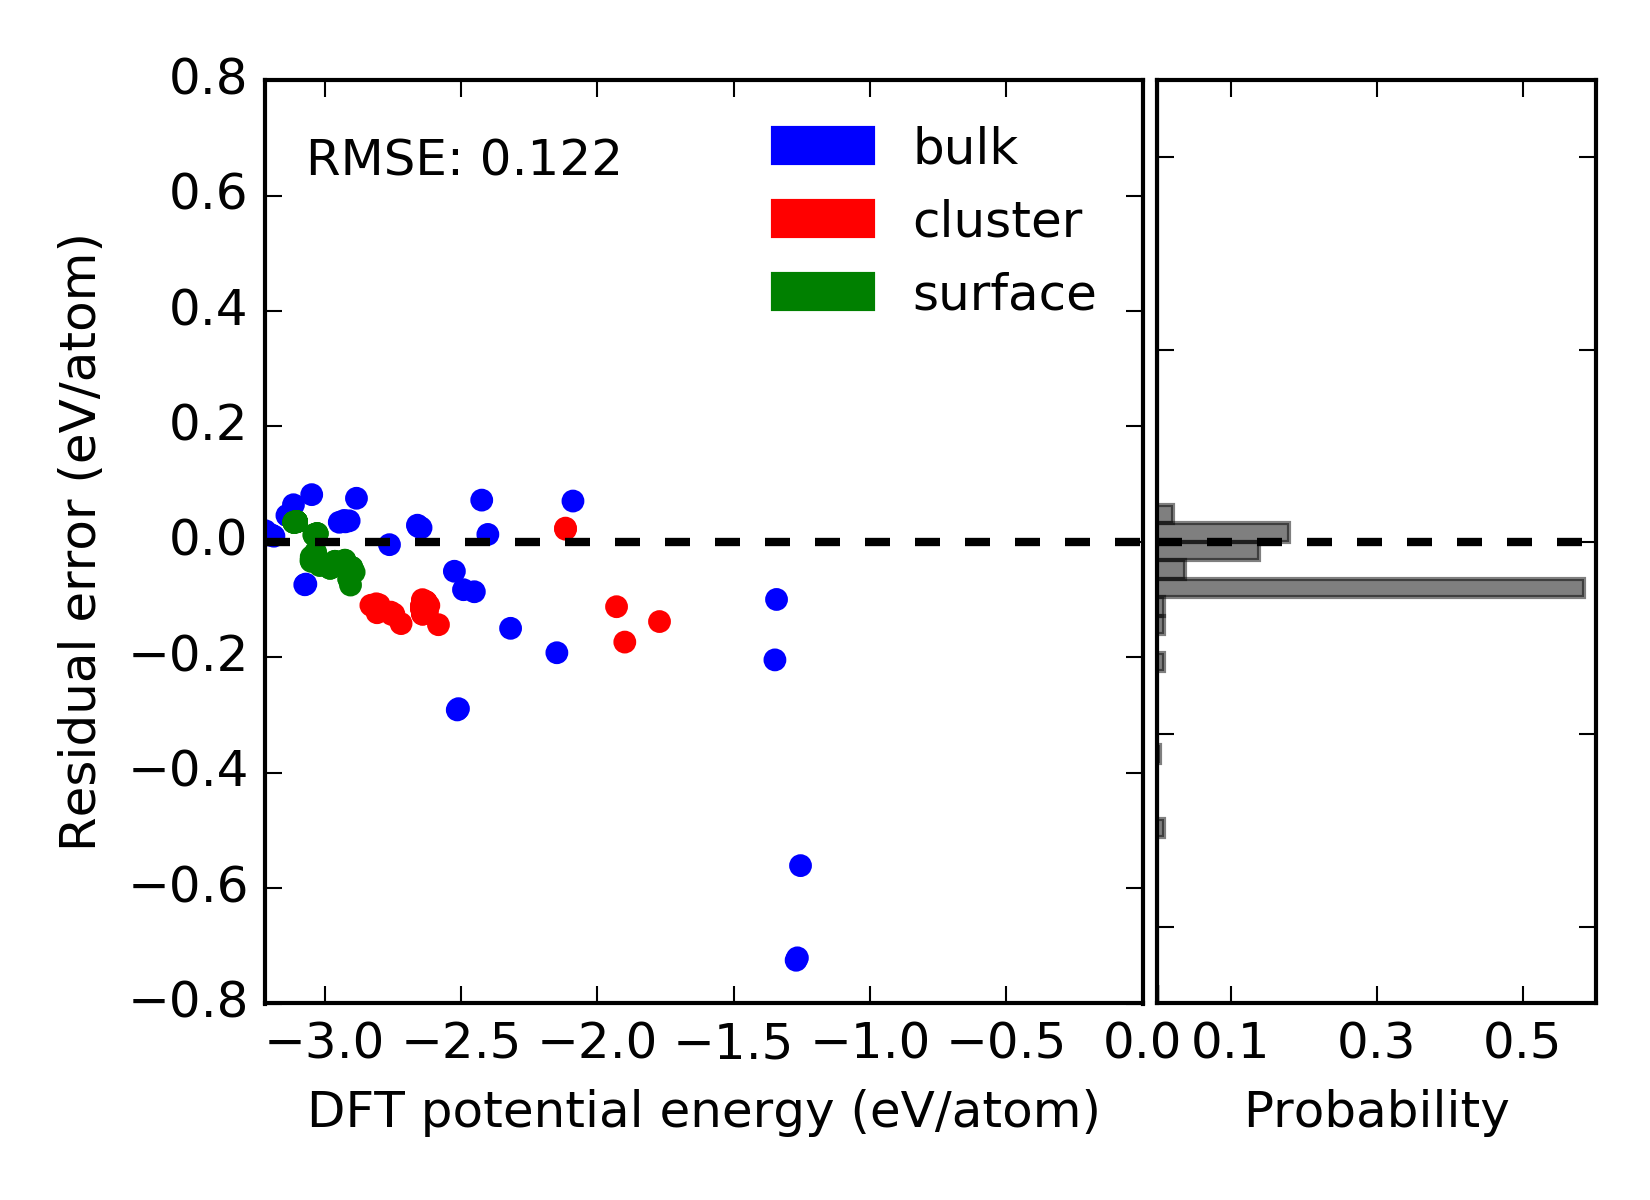
\includegraphics[width=5.5in]{./images/fig-reax-valid.png}
\caption{\label{fig-reax-valid}
Energy residual error to validation set data broken down by bulk, surface, and clusters for the ReaxFF potential.}
\end{figure}

\subsection{Neural Network}
\label{sec:orge351e71}
The NNs trained in this work were produced using the iterative training method outline in Chapter \ref{sec:ch3}. For Au, we used a cutoff radius, \(R\) = 6.5 \AA{} as long-range interactions are assumed to be negligible. (We find \(\approx\) 2 meV/nearest-neighbor energy differences between gas phase Au and a primitive fcc unit cell with 6.5 \AA{} nearest-neighbor distance). All NN used in this chapter contain 4 hidden layers with 40 nodes per layer and a hyperbolic tangent activation function.

Of the 9,972 total calculations, 9,734 were used for training the NN potential. Figure \ref{fig-neural-train} shows the error distribution from the training set. The mean, \(\mu\), and standard deviation, \(\sigma\), are given assuming a normal distribution fit. The RMSE is 0.017, similar to the standard deviation, indicating that the data is well approximated by a normal distribution overall.

\begin{figure}[h]
\centering
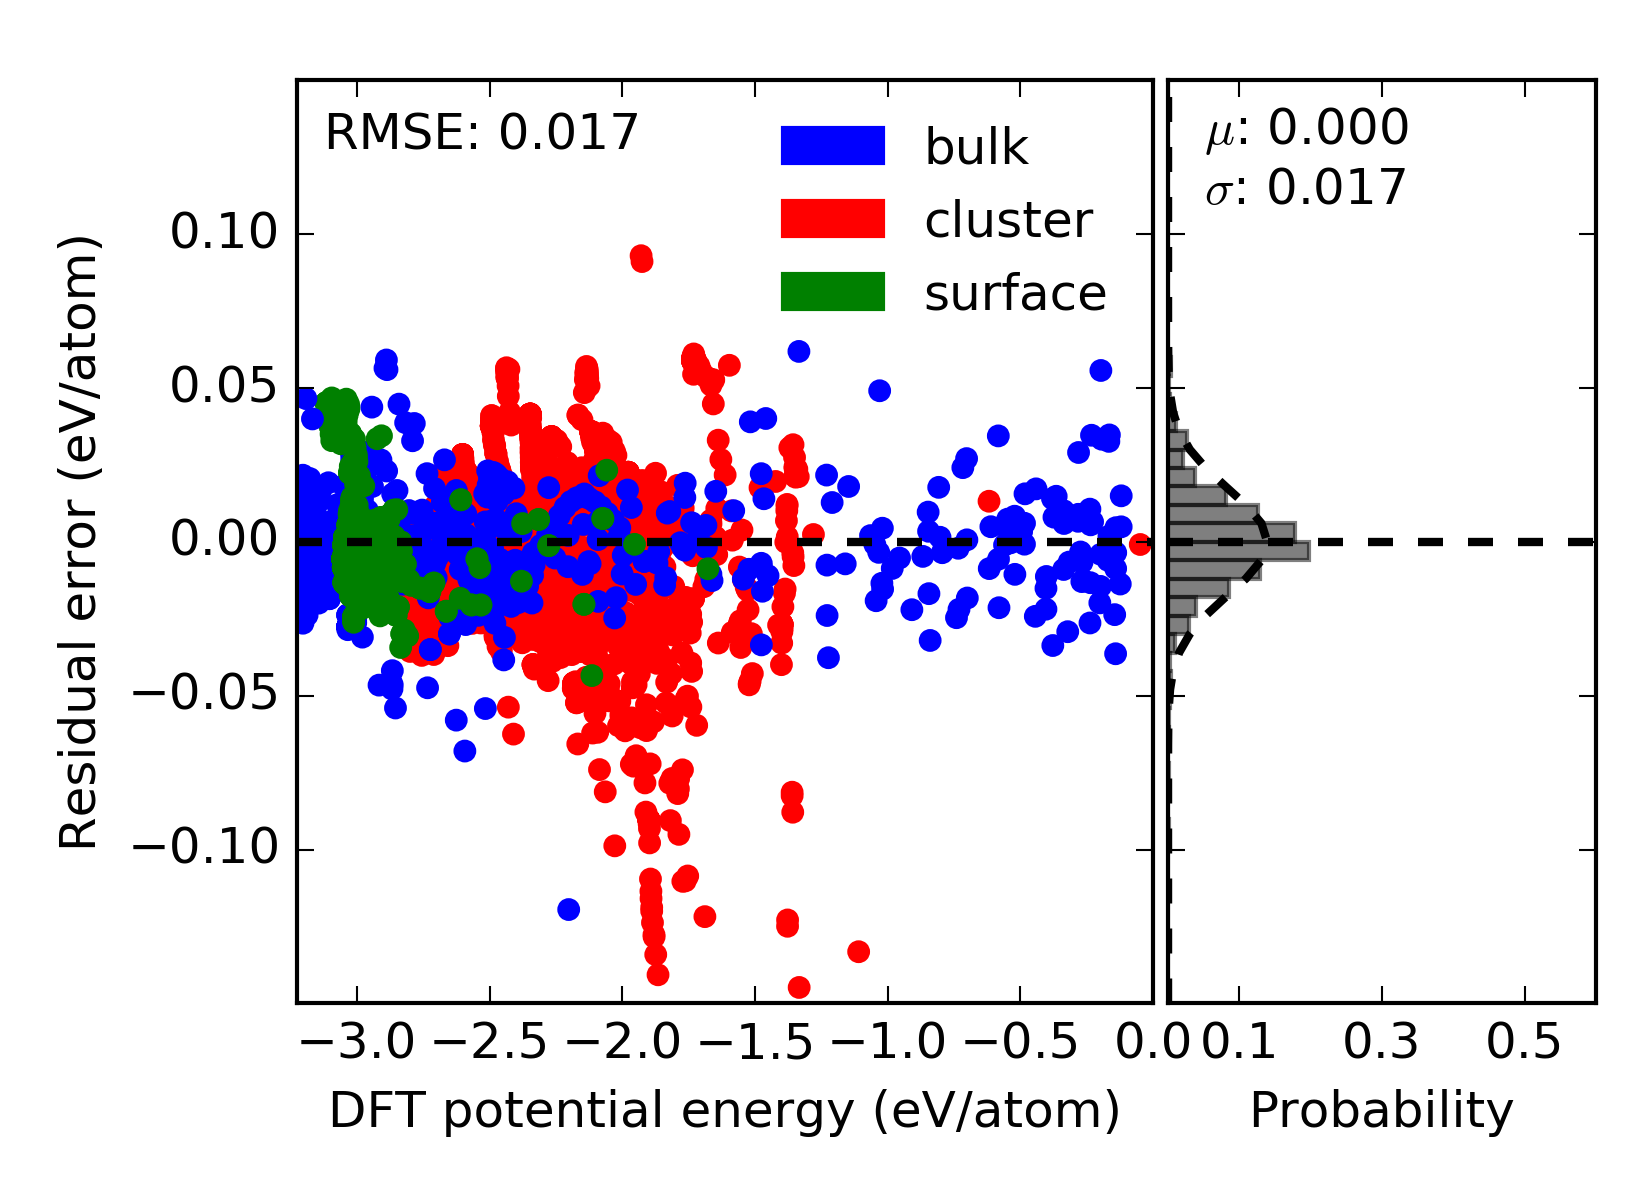
\includegraphics[width=5.5in]{./images/fig-neural-train.png}
\caption{\label{fig-neural-train}
Energy residual error to the training dataset of the NN calculations. A RMSE of 0.017 eV/atom is calculated for the 9,734 structures included in the training set. The training set is also well described by a normal distribution.}
\end{figure}

Figure \ref{fig-neural-valid} shows the error distribution for the validation dataset. Overfitting can be identified by a divergence between the RMSE of the training set and validation set data. In this case, the distribution is clearly not normal and arises from some underrepresented data in the training set, notably the fcc(100) terrace and dimer diffusion pathways (discussed below).

\begin{figure}[h]
\centering
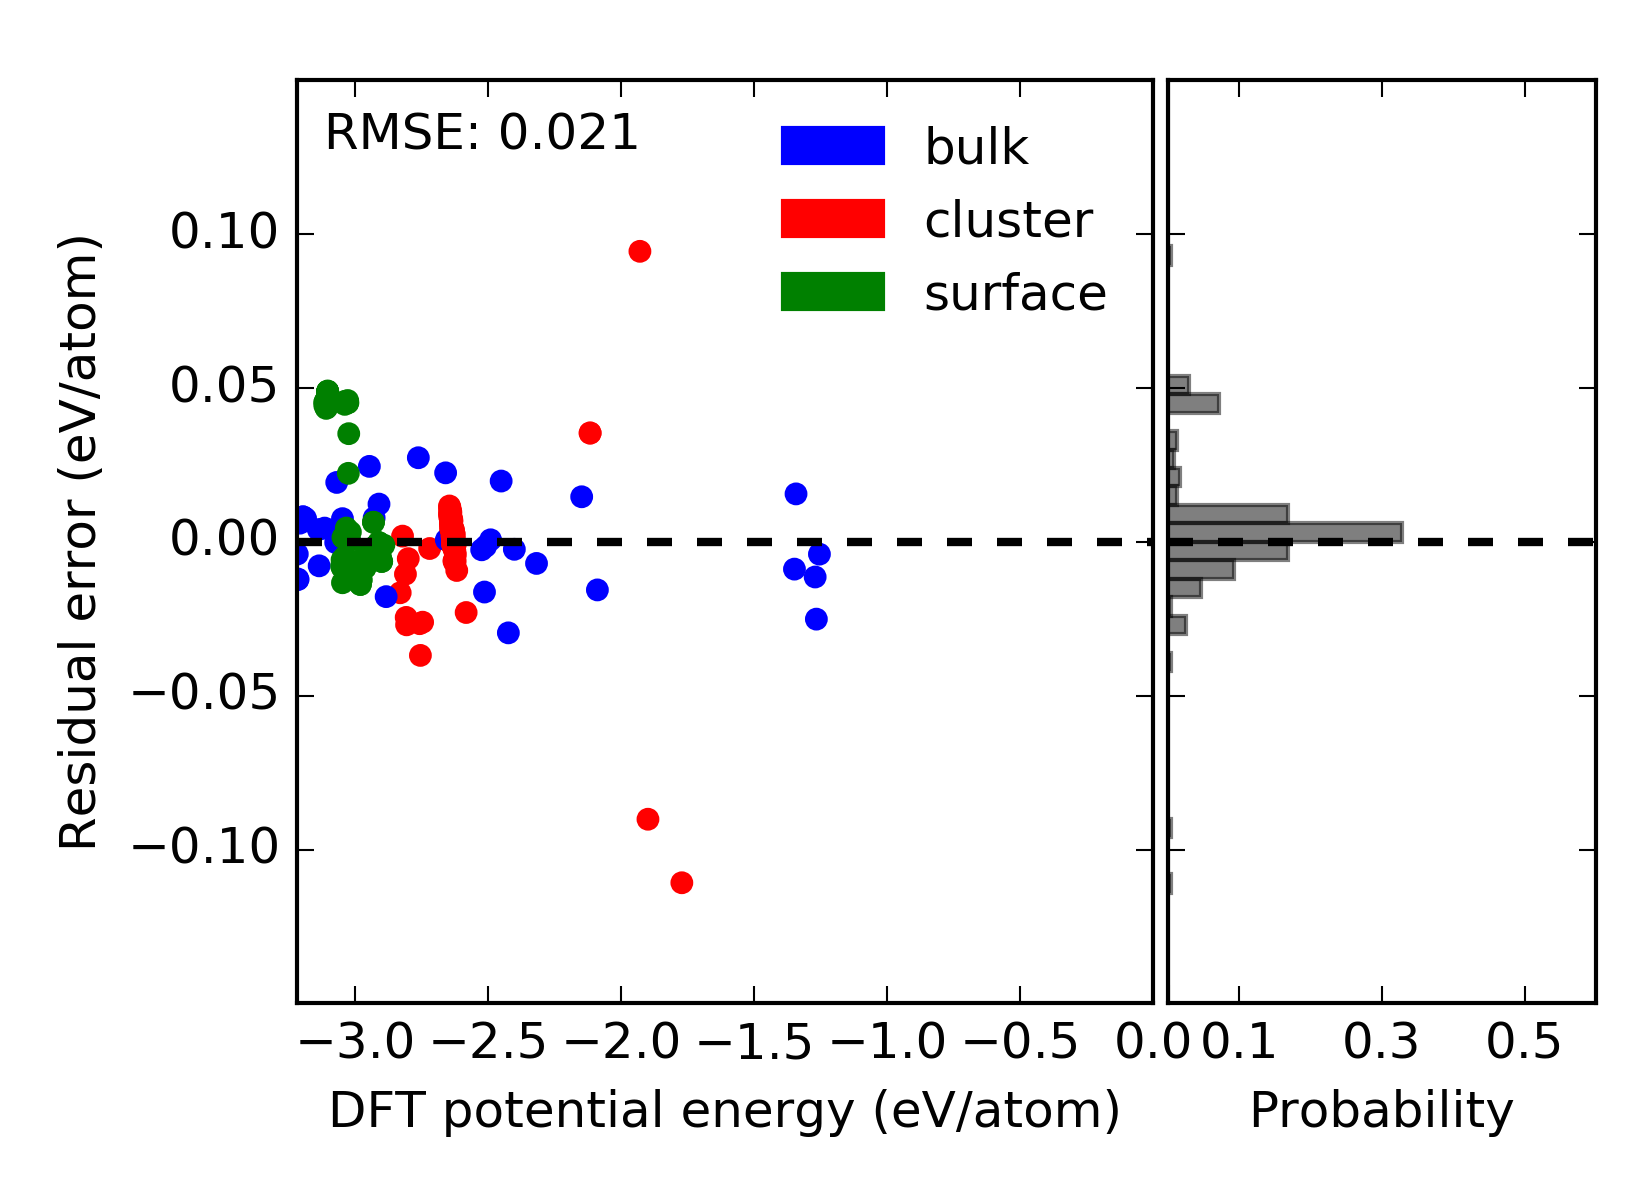
\includegraphics[width=5.5in]{./images/fig-neural-valid.png}
\caption{\label{fig-neural-valid}
Energy residual error to the validation dataset of NN calculations. \(\sigma\) = 0.21, similar to the training set RMSE indicating little to no overfitting has occurred. The cluster of overpredicted surface calculations are from fcc(100) surface diffusion pathways, which are poorly represented in the training set.}
\end{figure}

\section{Results and Discussion}
\label{sec:org01d607f}
We benchmarked the performance of the NN and ReaxFF potentials against DFT energies across three different material regimes: bulk, surface, and molecular cluster structures. Both of our generated potentials can provide reasonably accurate descriptions of Au in the different material regimes. In general we find that ReaxFF potentials are more readily overfit, less transferable to applications involving clusters of 126 atoms or fewer, and overall less accurate than the NN. However, ReaxFF potentials demonstrate a notable strength by predicting barrier heights that resemble those found in their training sets, when limited training data is available. NN potentials in general are significantly more accurate than ReaxFF potentials, but they require significantly larger training sets to ensure that accuracy. As explained below, they also currently bring substantially higher computational cost than ReaxFF potentials.

\subsection{Bulk properties}
\label{sec:org32df321}
\subsubsection{Equations of state}
\label{sec:org468c26f}
EOS data for face centered cubic, simple cubic, and diamond structures are shown in Figure \ref{fig-bulk-eos}. All training and validation calculations are fit to a 3rd order inverse polynomial \cite{alchagirov-2003-reply-commen}. The metrics for each fit are included in Table \ref{tbl-eos}. Results for the body centered cubic and hexagonal close packed EOS data are similar to the face centered cubic curve.

\begin{figure}[h]
\centering
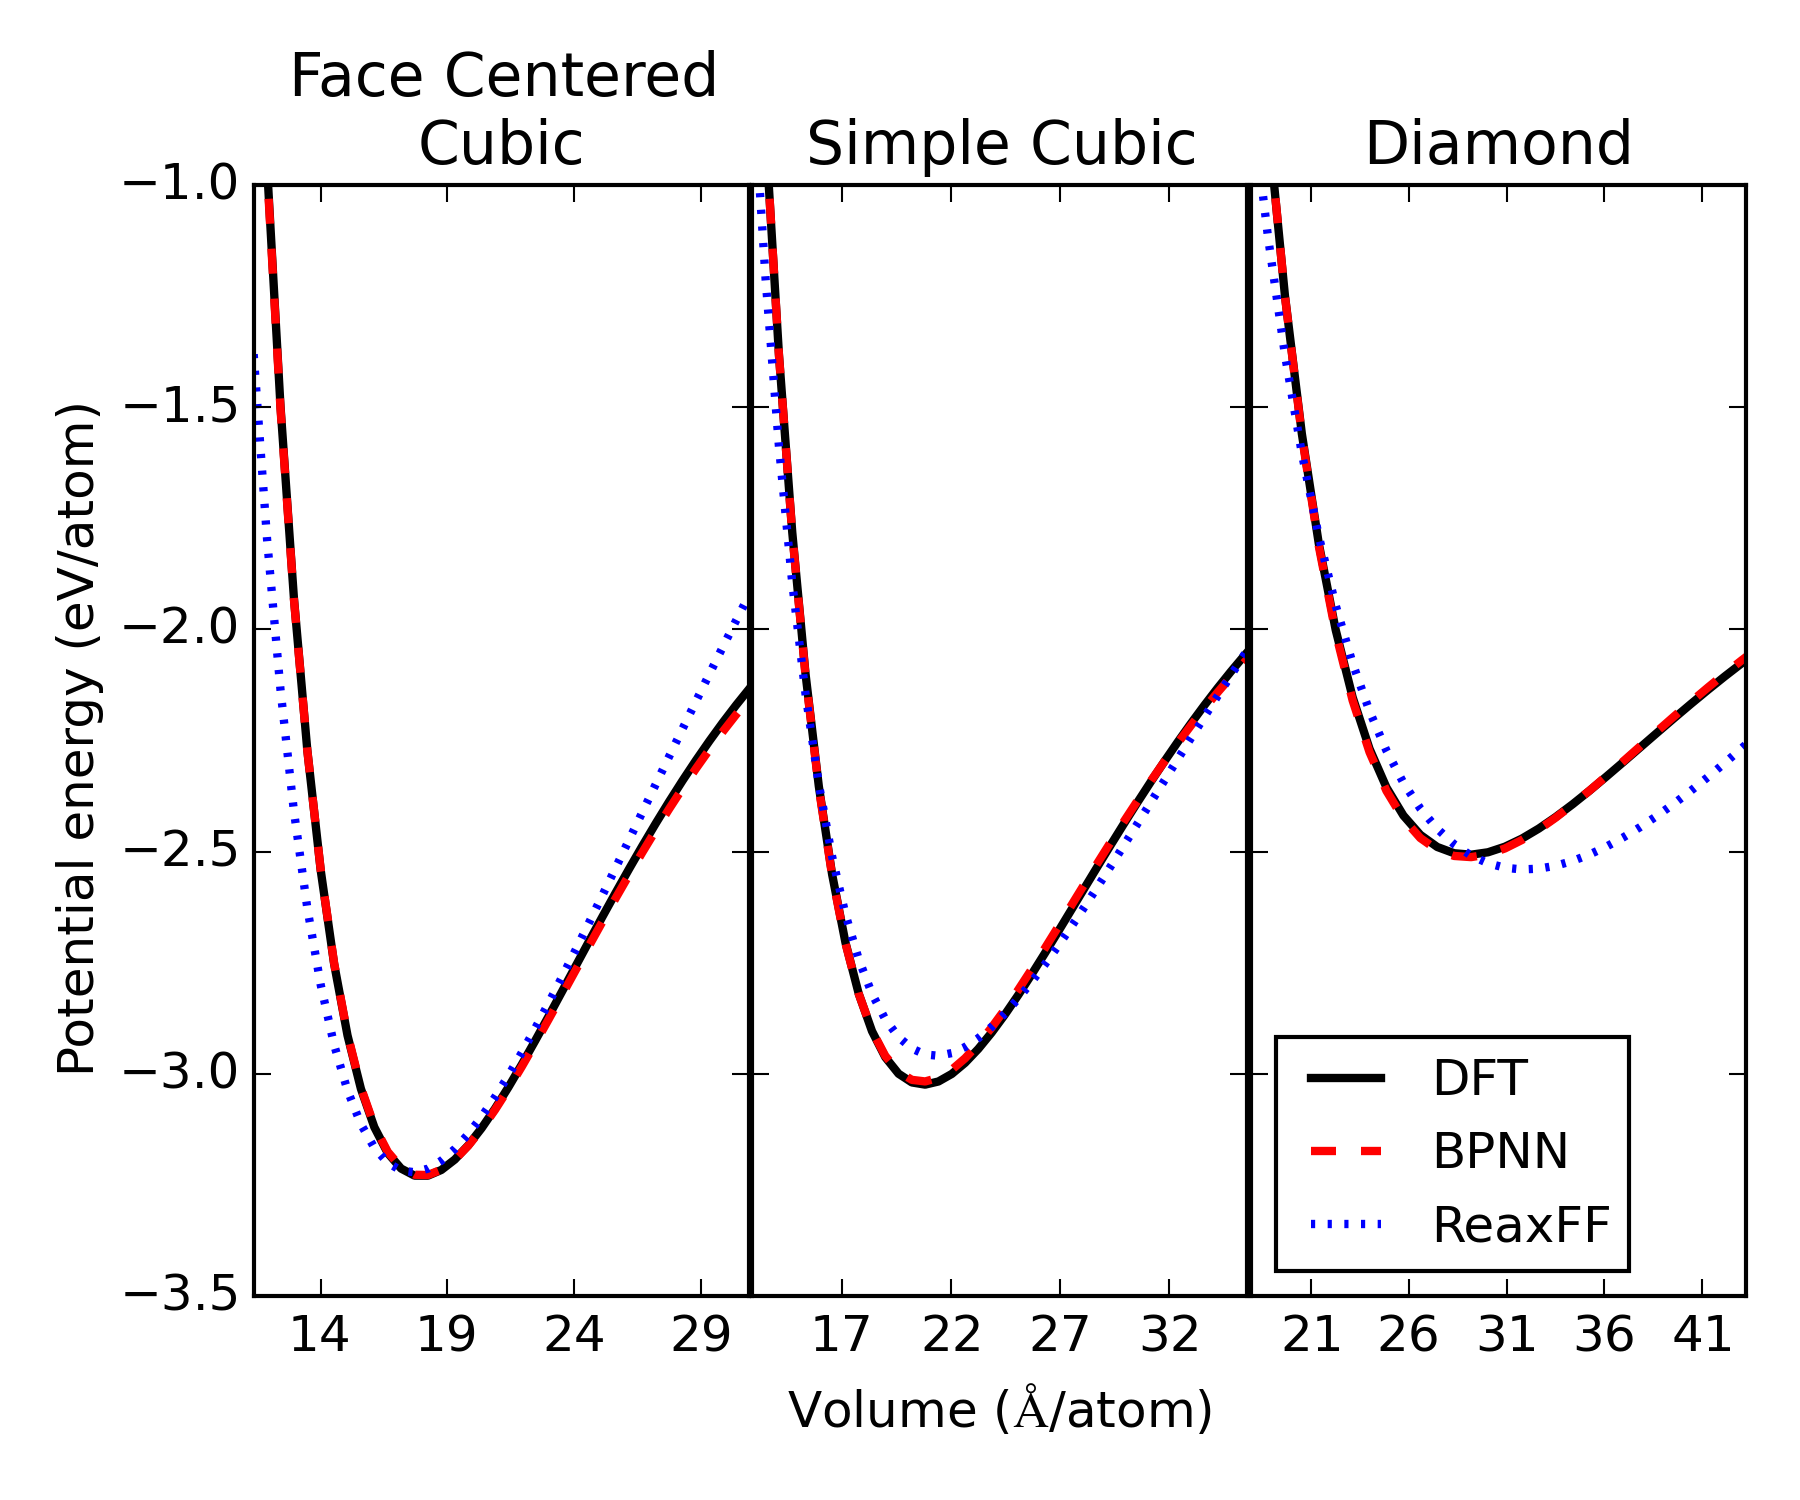
\includegraphics[width=5.5in]{./images/fig-bulk-eos.png}
\caption{\label{fig-bulk-eos}
Comparison of EOS fits to KS-DFT, ReaxFF, and NN training and validation set data. Fits only include data within atomic volumes of \textpm{} 15 \AA{}/atom as this is the region of interest for most applications.}
\end{figure}

Figure \ref{fig-bulk-eos} shows that the EOSs are very well represented by our NN potential. Validation set data are also well behaved, indicating that overfitting has not occurred. Metric data shown in Table \ref{tbl-eos} shows excellent agreement in the minimum volume, minimum energy, and bulk modulus found using DFT results. Data for the hcp and bcc structures shown in the SI of the published work are reproduced similarly well \cite{boes-2016-neural-networ}.

We find that ReaxFF potentials with 3-body terms have substantially better fits compared to force fields which do not include 3-body interactions (see \cite{keith-2010-react-forcef}). However, in both cases ReaxFF exhibits an unphysical convexity of the bond energy curve that creates problems manifested by large residual errors that can reach as high as \textpm{} 1 eV/atom at volumes away from the minimum energy volume. Many simulations sample regions in the vicinity surrounding the minimum volume, so these deviations are not shown in Figure \ref{fig-bulk-eos}. Data from Table \ref{tbl-eos} shows reasonably good agreement for the equilibrium volume and minimum energy of the three structures. Bulk moduli are underpredicted by \(\approx\) 20 GPa for each structure due to differences in the curvature of the EOS at the minimum. Again, one would likely improve the quality of predictions for individual properties by reweighting the parameterization to favor specific properties (e.g. bulk moduli), but this preferential fitting would also be expected to lower the quality of other predicted properties.

\begin{table}[h]
\caption{\label{tbl-eos}
Comparison of EOS metrics for DFT, ReaxFF, and NN fits as shown in Figure \ref{fig-bulk-eos}.}
\centering
\begin{tabular}{lrrr}
Structure & Min. volume (\AA{}\(^{\text{3}}\)) & Min. energy (eV) & Bulk Mod. (GPa)\\
\hline
DFT-fcc & 17.97 & -3.23 & 147\\
NN-fcc & 17.99 & -3.23 & 145\\
ReaxFF-fcc & 17.60 & -3.22 & 122\\
\hline
DFT-sc & 20.73 & -3.02 & 110\\
NN-sc & 20.66 & -3.02 & 110\\
ReaxFF-sc & 21.29 & -2.96 & 84\\
\hline
DFT-diam & 29.04 & -2.51 & 56\\
NN-diam & 28.98 & -2.51 & 57\\
ReaxFF-diam & 31.92 & -2.54 & 37\\
\hline
\end{tabular}
\end{table}

\subsubsection{Bulk vacancy formation and diffusion barrier}
\label{sec:org3af2eab}
Vacancy formation energies (\(E_v\)) are calculated using Equation \ref{eqn-vac}. \(E_f\), \(n_0\), and \(E_i\) are the energies of the structure with vacancy, number of atoms in the structure before forming the vacancy, and energy of the structure before forming the vacancy, respectively. Our DFT vacancy formation energies, shown in Figure \ref{fig-vacancy-formation}, are in good agreement with other GGA-PBE calculations (0.42 eV), but both sets of data significantly underpredict experimental results (0.93 eV) \cite{xing-2014-vacan-format}. This is likely due to the well-known shortcoming of GGA-PBE in underpredicting atomization energies of Au \cite{schimka-2013-lattic-const}. In this chapter, vacancy formation is referenced to the energy of a single atom in a primitive fcc unit cell. This may explain why the formation energies calculated here are slightly lower than those in the literature. The vacancies seem to reach the dilute concentration limit at \(\approx\) 0.037 vacancies/atom. The anomalous increase in energy for the structure at \(\approx\) 0.015 vacancies/atom is due to a minor structural perturbation into a different local minimum.

\begin{eqnarray}
E_v = E_f - \frac{n_0 - 1}{n_0} E_i \label{eqn-vac}
\end{eqnarray}

Our NN vacancy formation predictions are systematically overestimated by \(\approx\) 0.4 eV while ReaxFF vacancy formation predictions are systematically underestimated by \(\approx\) 0.3 eV. The preservation in trends indicates some error cancellation from the reference state for both fits. We find that neither method is sensitive enough to predict the subtle increase in energy for the reconfigured structure. Although the NN potential results are closer to experiment than the ReaxFF potential, this is simply a fortuitous error.  NN potentials have no physical basis and therefore would reproduce the DFT exactly with complete training.

The residual errors for structures with concentrations below 0.04 vacancies/atom are very low (less than 0.006 eV/atom, even for the point in the validation set having \(\approx\) 0.037 vacancies/atom). Error cancellation between the vacancy structures and reference structure make it difficult to determine the level of precision needed to obtain accurate vacancy formation energies. A NN potential for Cu has been constructed with a higher level of accuracy (error \(< 0.11\) eV), at the increased cost of a basis of calculations which is \(\approx\) 3.5 times larger \cite{artrith-2012-high}. NN calculations were also performed using unit cells of the same size as the corresponding vacancy structure. The same trend was observed with slightly higher formation energies using the expanded reference super cell.

\begin{figure}[h]
\centering
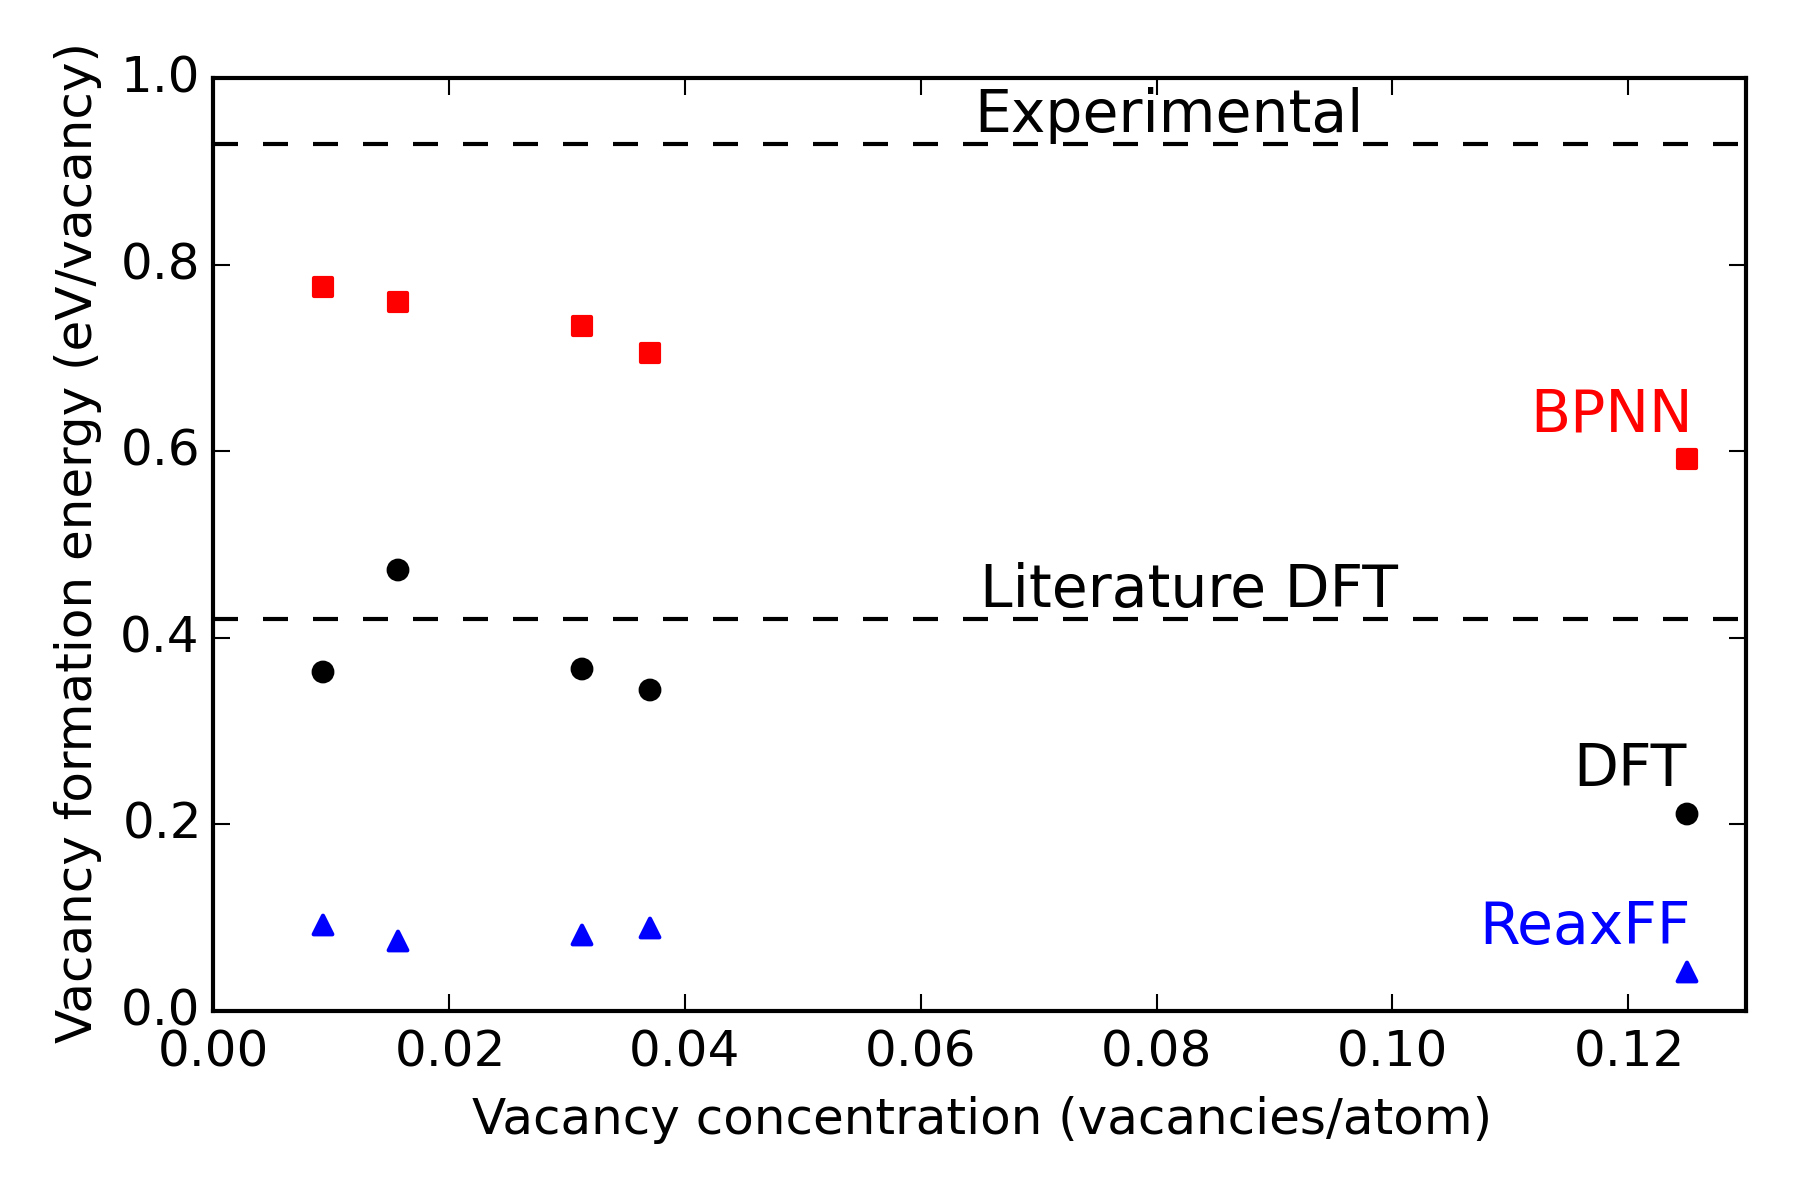
\includegraphics[width=5.5in]{./images/fig-vacancy-formation.png}
\caption{\label{fig-vacancy-formation}
Bulk vacancy formation energies for fcc Au at various concentrations. NN fits to vacancy structures are systematically overpredicted by \(\approx\) 0.4 eV, while ReaxFF fits are systematically underpredicted by \(\approx\) 0.3 eV. Literature values are from Ref. \citenum{xing-2014-vacan-format}.}
\end{figure}

Figure \ref{fig-vacancy-diffusion} shows the calculated bulk vacancy diffusion barrier using a vacancy concentration of \(\approx\) 0.037 vacancies/atom (obtained from Figure \ref{fig-vacancy-formation}). NEB calculations determined points along the minimum energy pathway that were then fit to a cubic spline. For diffusion calculations, the residual errors of both the NN and ReaxFF potentials are lower by about an order of magnitude as compared to the vacancy formation energy. This is due to error cancellation from the reference states that are similar to states along each reaction pathway. The NN potential overestimates this barrier by 0.04 eV while the ReaxFF potential underestimates the barrier by 0.05 eV.

\begin{figure}[h]
\centering
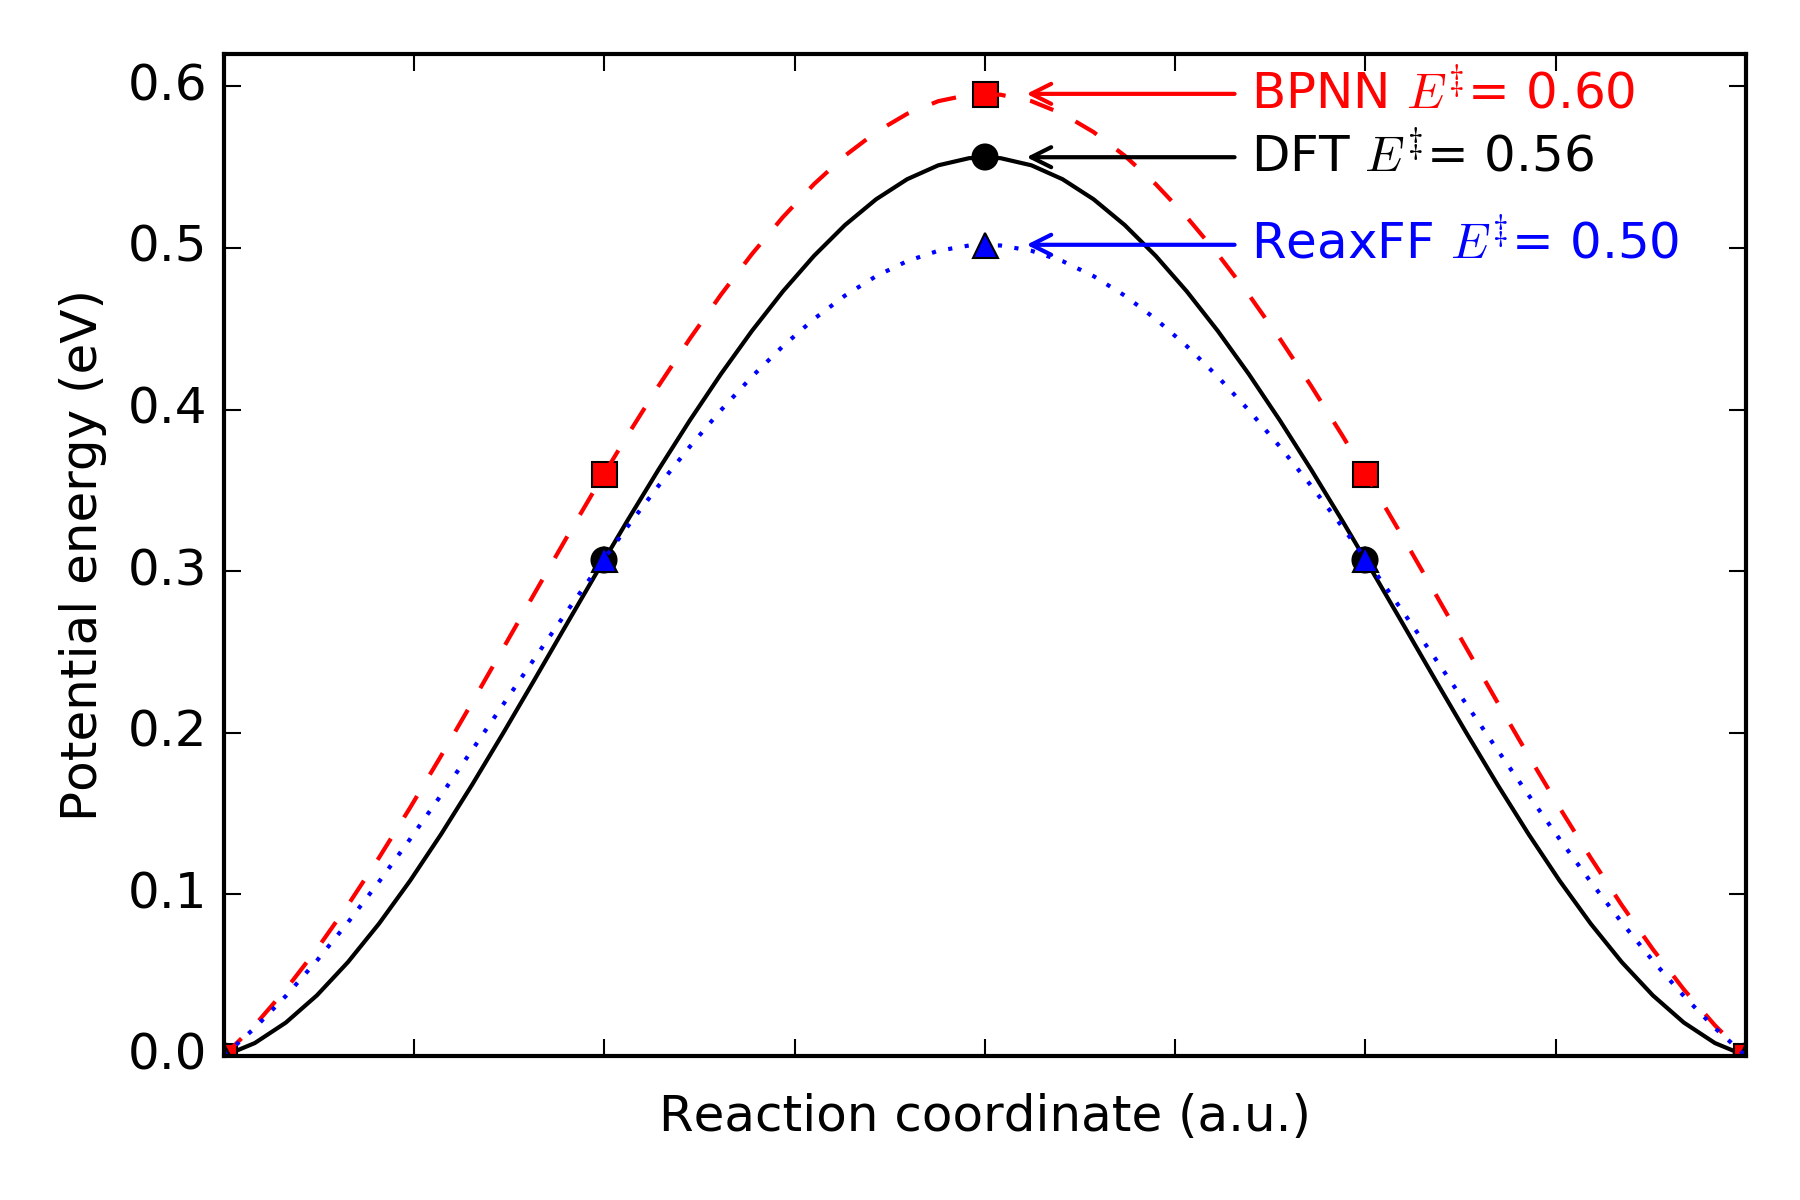
\includegraphics[width=5.5in]{./images/fig-vacancy-diffusion.png}
\caption{\label{fig-vacancy-diffusion}
NEB predicted barrier for bulk vacancy diffusion through fcc Au. Transitions state energy (black, 0.56 eV) is overpredicted by the NN (red, 0.60 eV) and underpredicted by the ReaxFF (blue, 0.50).}
\end{figure}

\subsection{Surface calculations}
\label{sec:orgdc940c6}
\subsubsection{fcc(100) diffusion barriers}
\label{sec:org33b30f5}
The training set for the ReaxFF potential in Reference \citenum{keith-2010-react-forcef} contains 166 surface diffusion barrier calculations from GGA-PBE using the SEQQUEST code \cite{schultz-2002-seqques}. NEB calculations with VASP were not used to recalculate the minimum energy pathways, but we recalculated single point energies on these structures using GGA-PBE in VASP to be consistent with the rest of our training set. Since NEB calculations were not done, there are significantly fewer points sampling the PES for these pathways compared to other pathways (8 - 10\texttimes{} fewer in most cases). Consequently, our NN fits to these pathways are expected to be less accurate compared to other pathways obtained from NEB calculations.

Figure \ref{fig-full-diffusion} contains recreations from Figure 2 (a \& b) in Ref. \citenum{keith-2010-react-forcef} using the NN potential and ReaxFF potential. Note that the terrace and dimer diffusion pathways are not included in the training set for either potential, and they represent predictions by both potentials. For the terrace diffusion pathway, the ReaxFF potential performs quite well and shows that the ReaxFF potential can provide very accurate predictions of barrier heights when the training set contains similar pathways. The NN potential, which contains more than 10\texttimes{} the training set data as the ReaxFF potential, can reasonably produce this adatom diffusion barrier but residuals fall between 0.2 - 0.3 eV. On the other hand, for a different adatom diffusion barrier, the NN potential predicts the dimer diffusion pathway quite well while the ReaxFF potential has higher residual errors between 0.1 - 0.2 eV. Larger training sets can be expected to reduce errors in both potentials, but reparameterization of these potentials with a larger training set will undoubtedly impact the accuracy when predicting other pathways.

\begin{figure}[h]
\centering
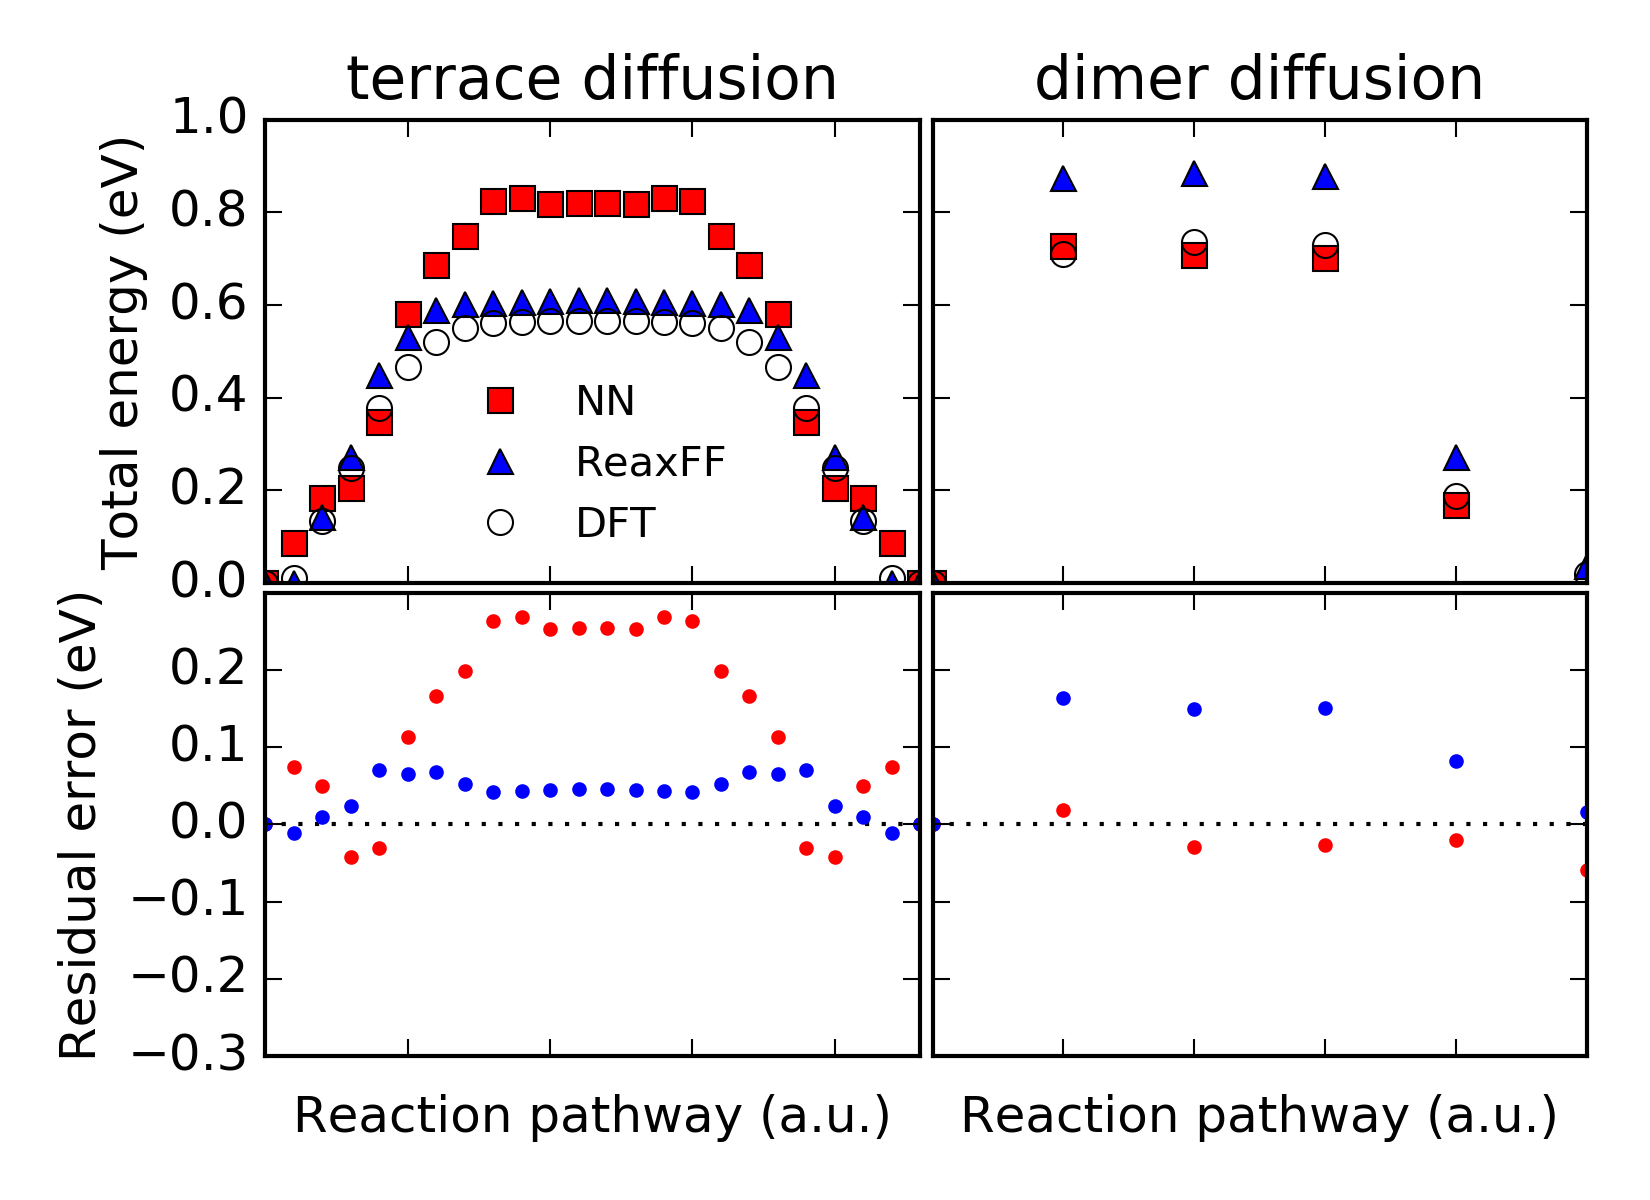
\includegraphics[width=5.5in]{./images/fig-full-diffusion.png}
\caption{\label{fig-full-diffusion}
Residuals to diffusion pathways in the validation set. Structures are reproduced from those used in Ref. \citenum{keith-2010-react-forcef}.}
\end{figure}

To assess the performance of these potentials under a wide range of adatom diffusions, Figure \ref{fig-barrier-residuals} shows the residuals for all 144 fcc(100) surface diffusion calculations. Solid shapes represent training set data and hollow shapes represent validation set data. Residuals are the same as those shown in Figure \ref{fig-full-diffusion}. Our ReaxFF potential (which has roughly 1/3 of its training set devoted to surface calculations) has 86.1\% of these structures falling within a \textpm{} 0.1 eV tolerance of error. For the NN potential (with roughly 1/10 of its training set devoted to surface calculations), has 52.1\% of these structures fall within a \textpm{} 0.1 eV tolerance of error.

Many of the calculations from the NN potential are underestimated compared to the reference KS-DFT data, signifying (as stated above) that these structures come from a poorly sampled region of the PES and improvements could be attained with more training. For the ReaxFF potential, errors appear to be less systematic, showing improved accuracy would require more training to specific pathways. In practice, both ReaxFF and NN potentials are normally trained with a specific application in mind, and so training sets, particularly those for ReaxFF potentials, can be smaller.

\begin{figure}[h]
\centering
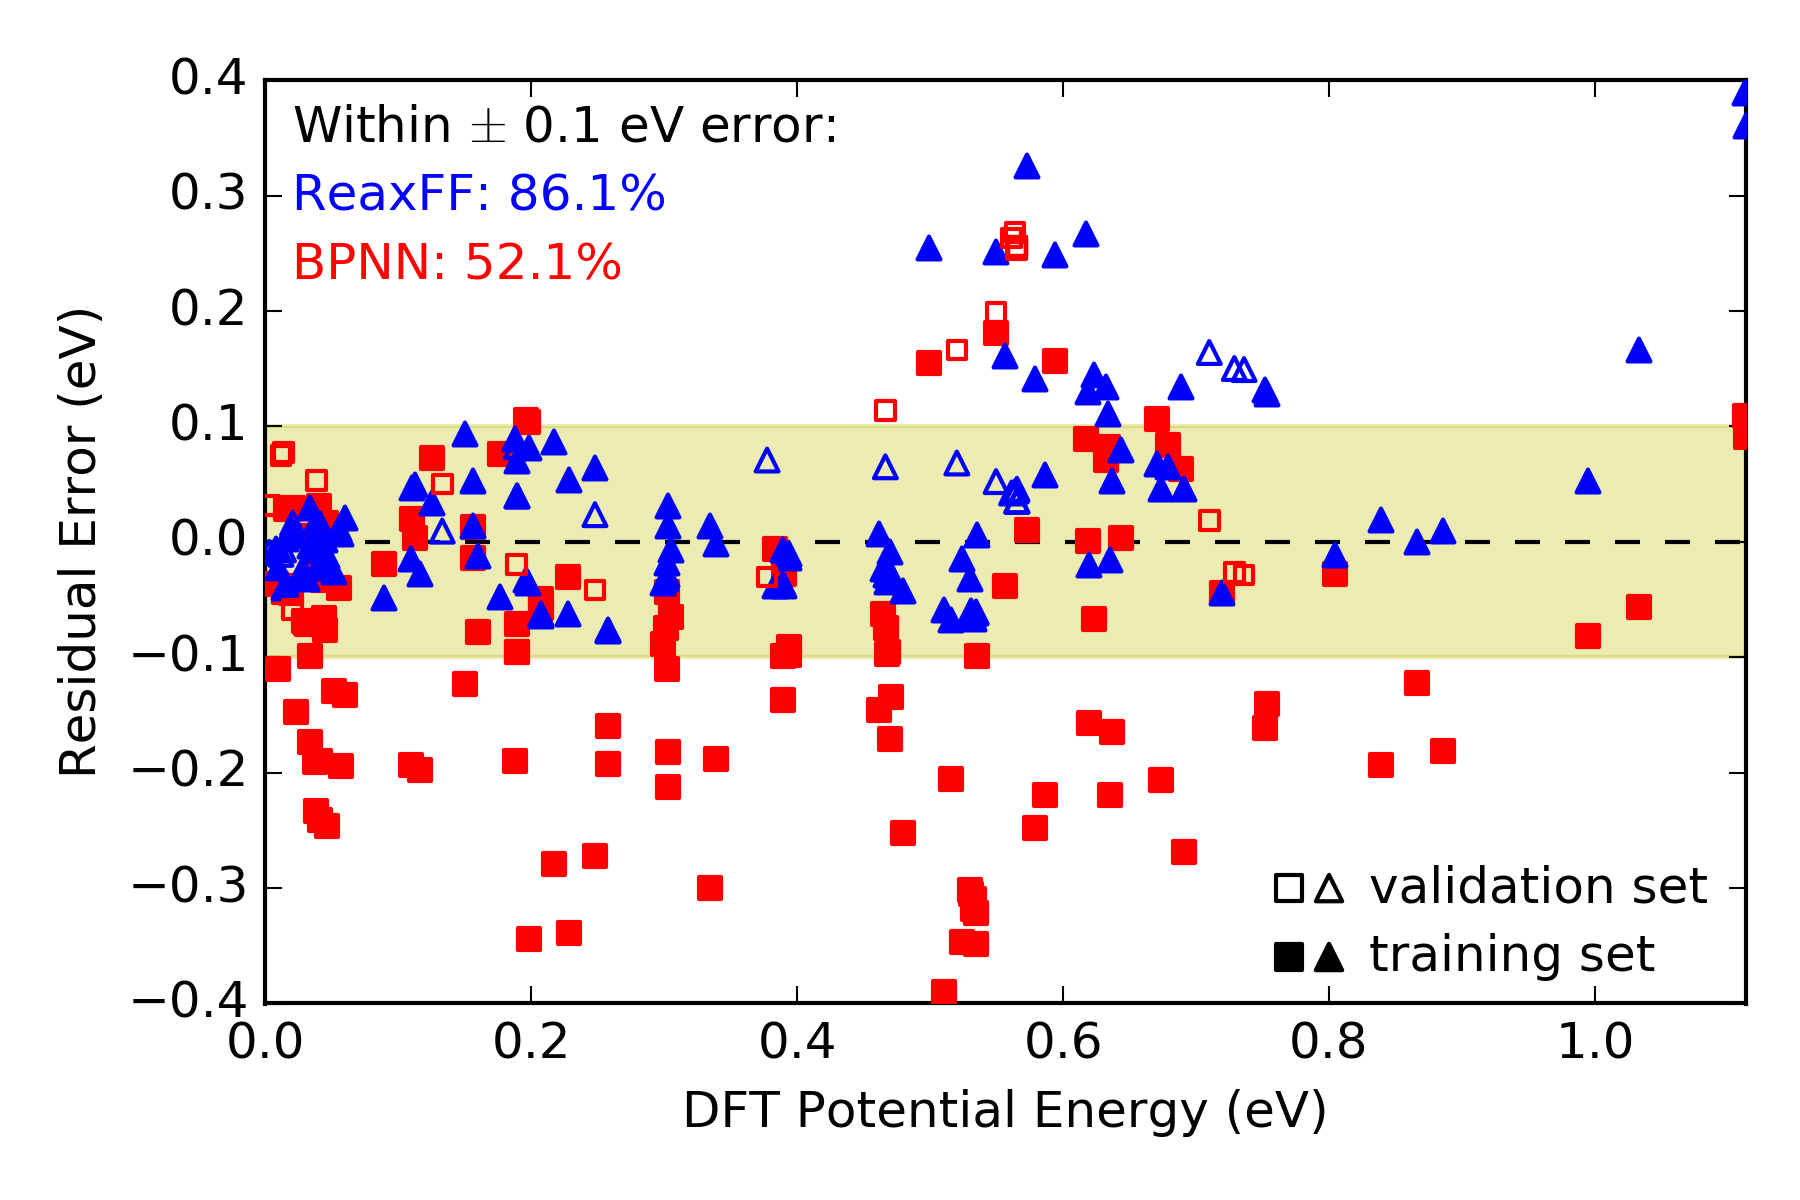
\includegraphics[width=5.5in]{./images/fig-barrier-residuals.png}
\caption{\label{fig-barrier-residuals}
Residuals of 144 fcc(100) surface diffusion pathway calculations included from Ref. \citenum{keith-2010-react-forcef}. Hollow markers represent residuals from the validation set which are shown in Figure \ref{fig-full-diffusion}.}
\end{figure}

\subsubsection{fcc(111) surface slipping barrier}
\label{sec:org8398ca3}
A slipping barrier is the minimum energy pathway required for a certain number of mono-layers of atoms to move from their ground state site to the next most adjacent site of the same kind. Slipping barriers were performed on fcc(100) and fcc(111) surfaces for one and two layers in a five layer slab. Figure \ref{fig-111-slipping} shows the single-layer slipping barrier for the fcc(111) surface. Both models find almost identical energies as DFT (within 0.05 eV). We can see that the ReaxFF potential finds a metastable intermediate instead of a single barrier as found by DFT and the NN potential. This ReaxFF potential also finds metastable intermediates when slipping in a different direction primarily over bridge sites, but residual errors are even lower. The very small difference in energies makes it difficult to assess if these are due to fitting errors or an unphysical component within the ReaxFF potential. Either way, both potentials can reproduce low energy slipping barriers within 0.05 eV with sufficient training.

\begin{figure}[h]
\centering
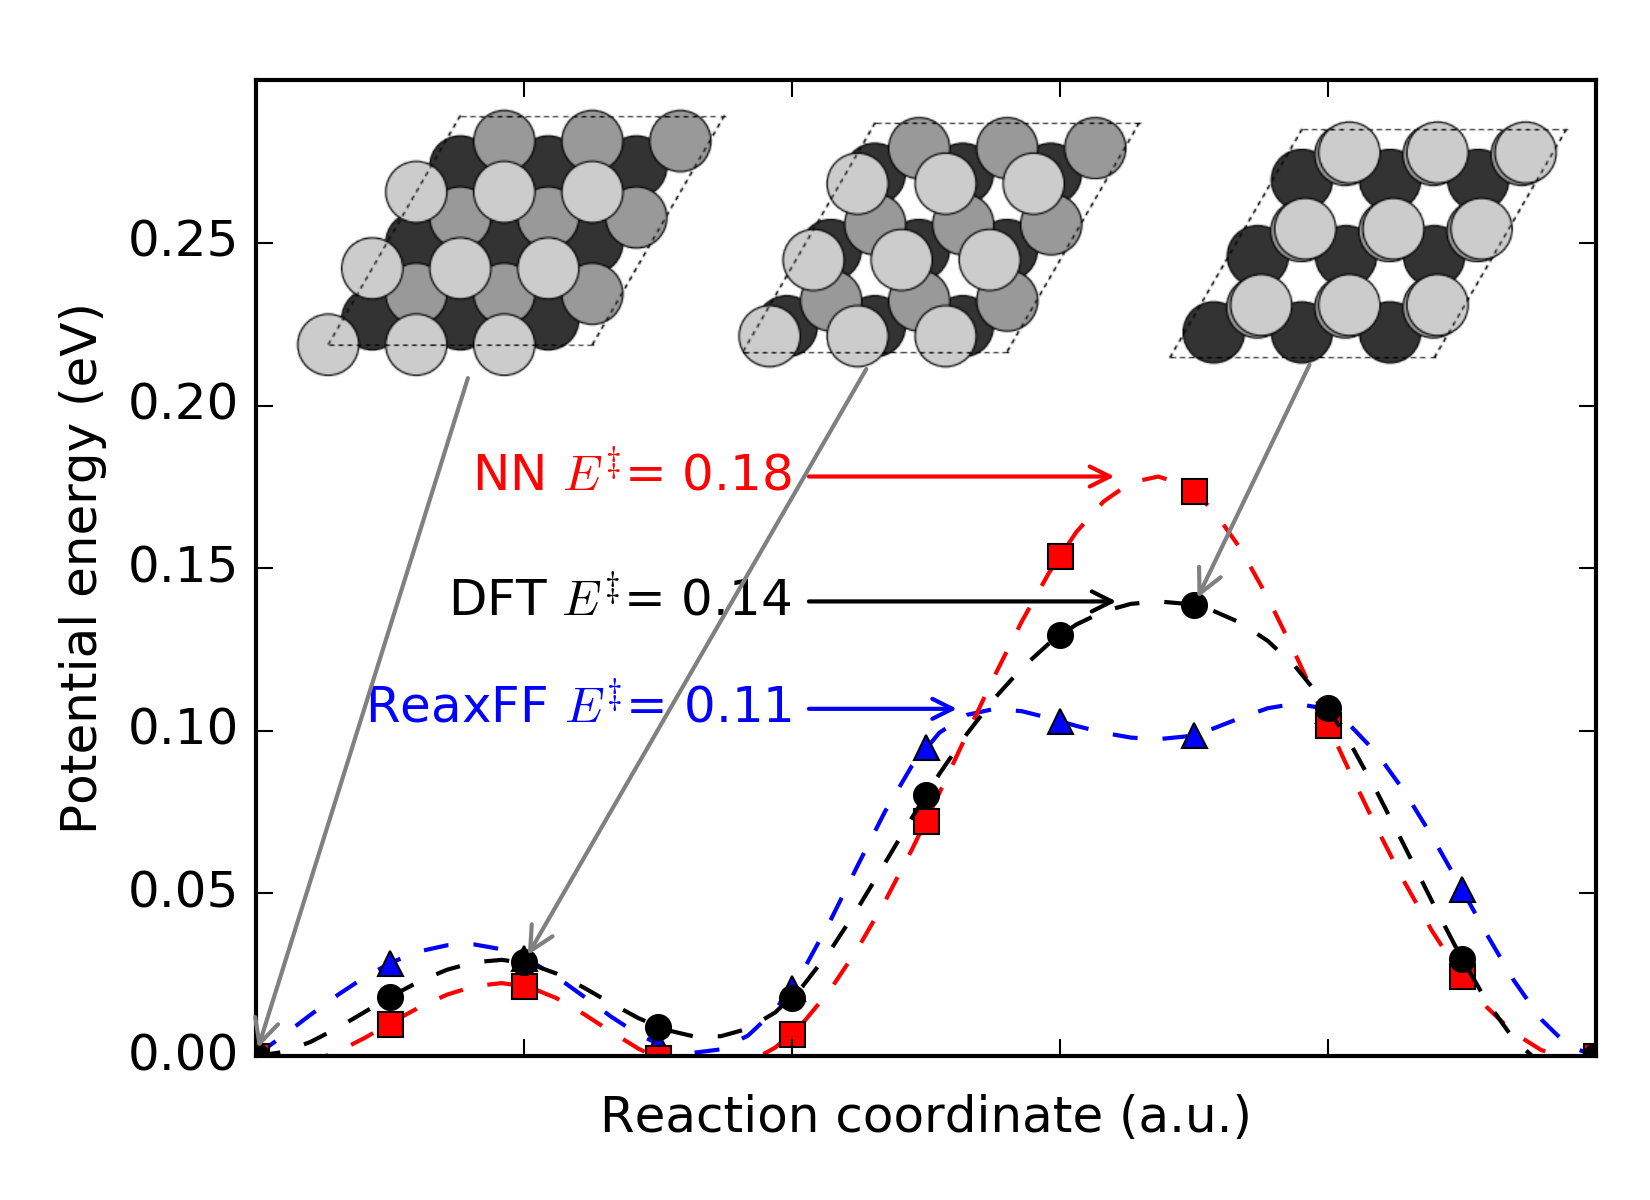
\includegraphics[width=5.5in]{./images/fig-111-slipping.png}
\caption{\label{fig-111-slipping}
NEB predicted slipping barrier for a single layer of fcc(111). Initial, bridge, and top positions are shown for visual reference. The second local minima is representative of the hcp site. The darkest gray represents the deepest layer, while the lightest shade is the top layer.}
\end{figure}
\subsection{Cluster predictions}
\label{sec:orgd28fae4}
\subsubsection{6 atom clusters}
\label{sec:org99e1e63}
Calculations on clusters up to 126 atoms make up \(\approx\) 81\% of the entire database. To determine the robustness of the NN potential for determining the energetics of structures not incorporated into the training set, several BO-MD simulations were performed on various clusters. For a six atom cluster, calculations were performed with NVT BO-MD without planar boundary conditions, where the temperature of the system was changed from 800 K to 300 K over the course of the simulation. The simulation using the NN potential started from a local minimum structure to determine if it would locate the known global minimum energy configuration. GGA-PBE found the global minimum to be planar and triangular (see Figure \ref{fig-6atom-md}), which is also observed in the literature \cite{phaisangittisakul-2012-stabl}. This structure was not included in the training set.

Figure \ref{fig-6atom-md} depicts the path taken by the NN BO-MD simulation (red) over the course of 2,000 time steps. Once every 100 steps we validated the energy using KS-DFT. The residuals are less than 0.05 eV/atoms for the NN potential, including the structure of the global minimum. We re-ran this simulation several times throughout development of the database. The first attempt at performing the described BO-MD simulation was with a dataset of \(\approx\) 2,000 cluster calculations with 20 atoms or fewer. In comparison with the full dataset, the residual error has been reduced dramatically, and the success rate of discovering the global minimum improved significantly. Further details of these initial attempts with the smaller database can be found in the SI file.

The 2,000 structures generated from the BO-MD run with our NN potential were then calculated using the ReaxFF potential. In this case, the ReaxFF potential did not identify the same minimum energy configuration of the six atom system. However, the cohesive energies of structures resembling the planar cluster are fairly consistent with KS-DFT data. Although the presented data shows situations where ReaxFF is not accurate, we note that this may signify an area where ReaxFF could be extended with additional functionality. For example, metal-metal bonds in small clusters could be treated with functional forms different than those used for bulk metal-metal bonds. This would likely correct systematic deviations, but such re-parameterizations may also adversely affect other structure types and/or increase computational cost. We note that Narayanan et al. have reported a hybrid bond order potential that uses a screened Lennard-Jones term for bulk structures in combination with a highly trained Tersoff potential for smaller regimes \cite{narayanan-2016-descr-diver}. This is a possible work-around to make other physical potentials accurate across different size regimes.

\begin{figure}[h]
\centering
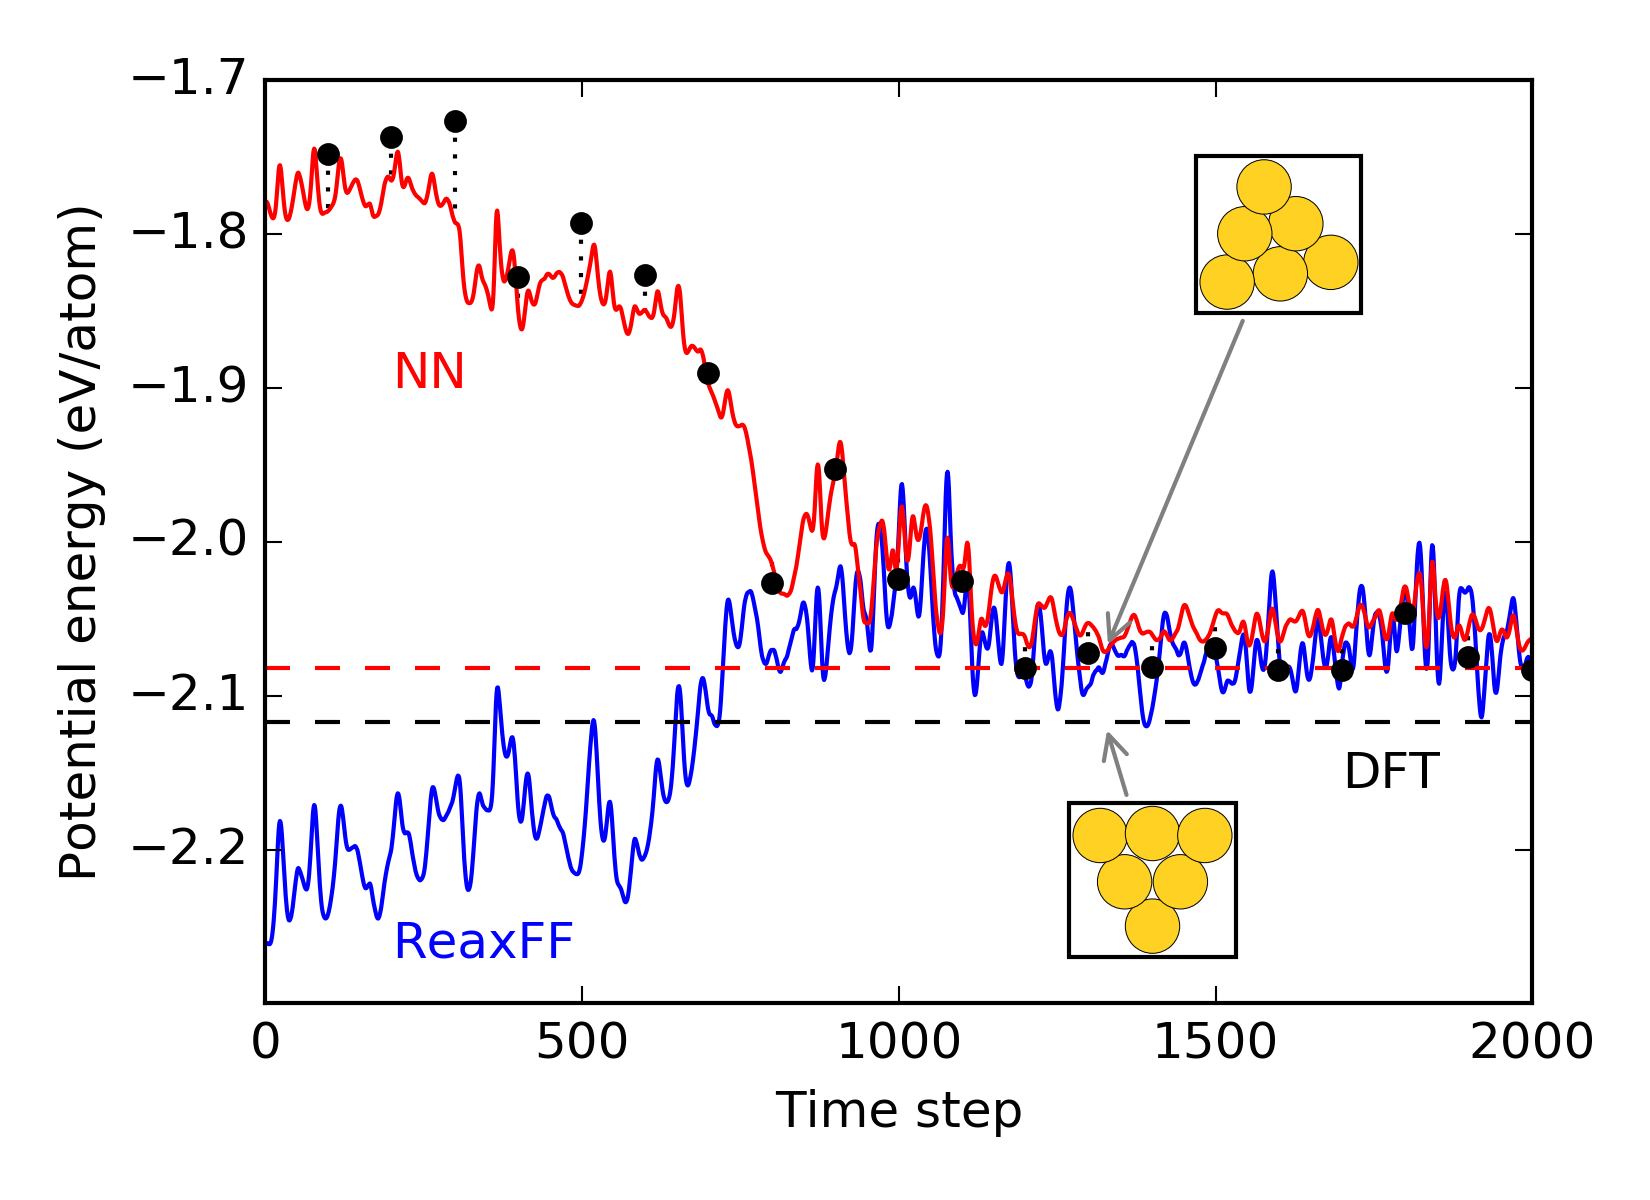
\includegraphics[width=5.5in]{./images/fig-6atom-md.png}
\caption{\label{fig-6atom-md}
NVT BO-MD simulation of 6 atom cluster starting from local energy minimum and finding the global minimum. The temperature was reduced from 800 K to 300 K over the course of the simulation. Solid lines show BO-MD trajectories while dashed lines show energy predictions for the global minima from KS-DFT (black) and NN (red) and ReaxFF (blue).}
\end{figure}

\subsubsection{38 atom clusters}
\label{sec:org0c0e826}
A similar exploration for multiple local minima was implemented on a 38 atom cluster using minima hopping techniques \cite{goedecker-2004-minim}. This exploration of minimum energy structures works through a series of fixed temperature NVT BO-MD simulations followed by geometric optimization requiring a significant number of calculations between each iteration. After each iteration, the minimum geometry is stored and perturbed before restarting its search. The resulting minima predicted from 125 such iterations are shown in Figure \ref{fig-38atom-minima}.

Again, this approach located a lower energy minimum than the starting point geometry. The largest energy difference between minima occurred during the first iteration of the process. After this initial step, the energies do not change as dramatically. This can be interpreted as a shift into a local minimum energy basin (a group of configurations with similar atomic positions and energies) which the NN potential proceeds to explore in the next 124 minima. A more complete analysis of the 38 atom Au cluster space would be time consuming and is beyond the scope of this work. Despite demonstrating low residual errors, the NN potential does not correctly predict the lowest energy structure determined by KS-DFT in this set of minima. Regardless, it is still capable of distinguishing between configurations in different basins, and thus could be a valuable tool for exploring minimum energy structures in conjunction with KS-DFT calculations.

Residual errors for the ReaxFF potential are consistently lower by -0.11 eV/atom compared to KS-DFT. If energetics are shifted by this amount (as show in the top of Figure \ref{fig-38atom-minima}) one finds that the trend in relative energies is in reasonable agreement with KS-DFT, although our ReaxFF potential does not correctly predict the lowest energy configuration either. The performance of the ReaxFF potential for clusters could always be improved by adding more cluster data to its training set, but we found that doing so rapidly deteriorates its ability to calculate bulk and surface properties. As a result, we do not recommend using ReaxFF in its standard formalism for applications involving clusters with fewer than 126 atoms.

\begin{figure}[h]
\centering
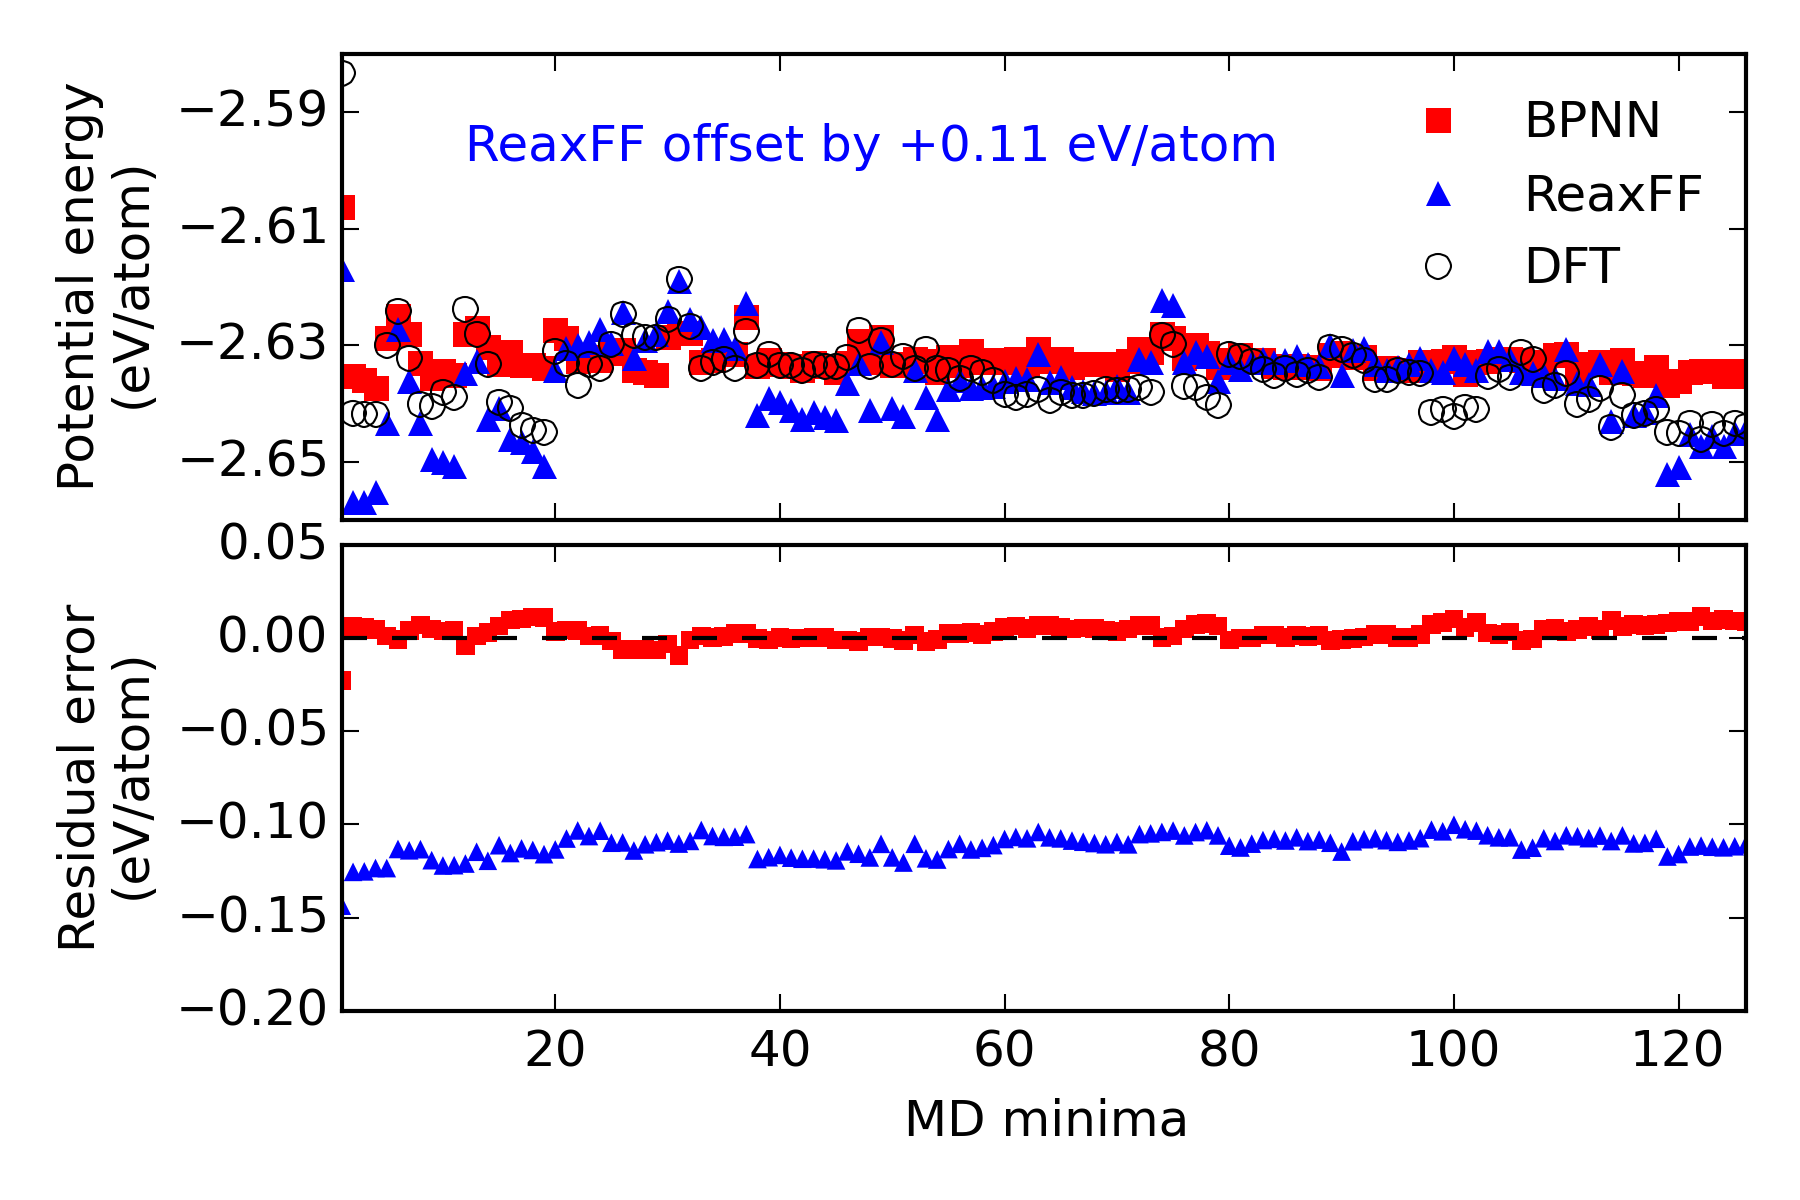
\includegraphics[width=5.5in]{./images/fig-38atom-minima.png}
\caption{\label{fig-38atom-minima}
Local minima for 38 atom Au cluster predicted from the NN (red) and compared with KS-DFT (black) and ReaxFF (blue). The ReaxFF potential energies are offset by +0.11 eV/atom in the top figure to better depict the trend in energies.}
\end{figure}

\subsection{Computational cost}
\label{sec:org2df75d9}
An important aspect of these modeling approaches is their computational cost. This includes the time needed to produce the necessary QC training sets, train the potentials, and the time needed to run the calculations. Implementation and training of parameters for the NN potentials can be automated using instructions in the SI file of the published work \cite{boes-2016-neural-networ}, thus reducing the time needed to learn how to train potentials. The generation of meaningful QC data is also a significant bottleneck in time, particularly for NN potentials that require large training sets to be accurate. This is simplified in part by generating NEB data and geometry optimizations which contain many valuable calculations on which physical and mathematical potentials can be trained. One of the best ways to speed the progress of developing accurate and transferable potentials is to make data and methods freely available and easily accessible.

A fair comparison between calculation times between ReaxFF and NN potentials is not currently possible. The NN potential we developed used a Python code that is still in early stages of development \cite{khorshidi-2016-amp}. In comparison, ReaxFFs and other force field codes have been implemented in the LAMMPS program which is already a high performance computing code. \cite{plimpton-1995-fast-paral}. Using available open source tools, BO-MD simulations on the 6 atom cluster using the C-compiled ReaxFF code performs \(\approx\) 6,700 timesteps/second, while the Python NN in ASE performs \(\approx\) 15 timesteps/second. Nevertheless, we consider NN potentials to be extremely promising for simulations requiring high accuracy, especially if they can be implemented into high performance codes that can dramatically accelerate their calculation times.

\section{Conclusions}
\label{sec:org897f9e1}
We have trained ReaxFF and NN potentials using subsets of \(\approx\) 10,000 DFT calculations. Our training sets consider Au in a variety of atomic configurations in bulk, surface, and cluster regimes that would be useful for practical atomistic modeling across all regimes. By virtue of being a mathematical potential, the NN potential can be trained to an arbitrary level of accuracy. Our most accurate NN potential was fitted to 9,734 calculations and yields an RMSE of 0.017 eV. Our ReaxFF potential (which contains 3-bond terms for higher accuracy) was fitted best to a significantly smaller training set consisting of 848 calculations (a value that is considerably larger than parameter sets in many other ReaxFF potentials). This potential provides an overall RMSE of 0.136 eV compared to the full DFT dataset.

In applications on bulk structures, our NN almost exactly reproduces reference DFT data of equations of state, while the ReaxFF potential is less accurate, particularly at atomic volumes that extend far beyond the equilibrium structures. When modeling surface structures and adatom diffusions, both the ReaxFF and NN potentials perform quite well with sufficient training, but obtaining a NN potential having comparable or higher accuracy than ReaxFF for adatom diffusions requires substantially larger training sets. For clusters, the NN potential exhibits essentially negligible residual errors compared to the KS-DFT calculations it was trained to, while the ReaxFF potential exhibits sizable systematic errors of 0.11 eV. This highlights the challenge of developing a physical potential that is accurate across bulk, surface, and cluster data. Increasing the size of the training set for the ReaxFF potential to include more cluster data was found to be detrimental to the accuracy of bulk and surface data, thus showing an area needing improvement in terms of ReaxFF functionality.

Although NNs can be trained to the desired level of accuracy, the computational cost, both upfront in the form of training set data and during calculation time, are currently substantially higher than ReaxFF potentials. Nevertheless, NN potentials are very promising if trained for specific applications (hence requiring smaller training sets) and they will be increasingly useful as computational developments enable faster runtimes. Since accurate NN potentials contain substantially larger numbers of parameters than most physical potentials, it is unlikely that NN potentials will ever be as fast as ReaxFF potentials, but we have demonstrated that NN potentials can be trained to be substantially more accurate.

\chapter{Neural Network Predictions of Oxygen Interactions on a Dynamic Pd Surface}
\label{sec:ch5}
\section{Introduction}
\label{sec:org753cce4}
In this chapter, we have created a Behler-Parrinello NN trained to 11,925 DFT calculations which consist of the Pd(111) surface facet and adsorbed oxygen coverages from 0-1 ML. Only Cartesian NNs have been implemented for studying surface interactions such as oxygen on Al \cite{behler-2007-repres-molec}. Behler-Parrinello NNs have studied single element systems (\emph{e.g.} Si, C, and Au \cite{behler-2008-metad-simul,eshet-2010-ab,boes-2016-neural-networ}), and in those works they were primarily used to model bulk properties. They have also been used to study various fcc facets of the Cu surface \cite{artrith-2012-high} and alloy nanoparticle interactions with water \cite{artrith-2015-grand-cu}. We have previously studied oxygen adsorption on Pd(111) \cite{kitchin-2009-correl-cover} and others have used a cluster expansion to model the coverage dependence \cite{frey-2014-implic-cover}. In this work, we demonstrate that a NN can also be used, and that it has some advantages over other approaches.

With the best performing NN produced, we demonstrate how this method can be utilized to bridge limitations in both the classic Cartesian NN framework, and also cluster expansion techniques. We do this by demonstrating various coverage-dependent interactions of oxygen on a dynamic Pd(111) slab. This includes NEB pathways \cite{henkelman-2000} of oxygen diffusion and self-interaction, MD simulations of low oxygen coverages, and grand-canonical MC simulations of adsorption at the fcc hollow site.

\section{Methods}
\label{sec:org7846c70}
\subsection{Density Functional Theory}
\label{sec:ch5-dft}
Monkhorst-Pack \emph{k}-point grids \cite{monkhorst-1976-special-point} were used  and the Kohn-Sham orbitals were expanded up to energy cutoffs of at least 400 eV. For structures containing oxygen, an energy cutoff of 800 eV was used. This high energy cutoff was chosen based on convergence studies performed on an oxygen molecule in the gas phase. All convergence criteria were chosen to attain an energy convergence of at least 1 meV/atom in the DFT calculations. Transition states reported are calculated using the climbing image NEB method \cite{henkelman-2000}. Instructions on how to access the complete database of calculations can be found in the SI file of the published work \cite{boes-2017-neural-networ}, along with more details on the methods used in this work.

To sample the PES of PdO surface interactions we began with fcc site enumerations on 3 \texttimes{} 3 \texttimes{} 4 Pd slab. In this way we can directly enumerate all of the various coverage configurations, of which there are 512. Many of these configurations are not energetically unique due to the symmetry of the system. To prevent training the NN to a large number of energetically degenerate configurations, Effective Medium Theory (EMT) \cite{jacobsen-1996-semi-empir} was used to identify energy unique configurations. This process is outlined in more detail in the SI of the published work \cite{boes-2017-neural-networ}. This process was repeated for all possible hcp, bridge, and top sites of the same Pd slab. After the unique structures were identified, the bottom two layers were held fixed at the lattice constant calculated for pure bulk Pd (3.939 \AA{}) before performing full relaxations. Each relaxation step was used as training data for the first iteration of the NN implemented in this work. Once a feasible NN potential was generated, the majority of the remaining data was created by utilizing the potential for MD and further coverage calculations. The final database includes 11,925 calculations. Select bulk Pd calculations are also included to improve fits of clean Pd slabs.

\subsection{Neural Network}
\label{sec:org9aff7a4}
In this chapter, we use a cutoff radius, \(R\) = 6.5 \AA{}. This value is chosen based on DFT results for the equation of state of an oxygen dimer and the equation of state for Pd extended to the dilute limit. There is no change in the total energy of the oxygen system at a distance of \(\approx\) 4.5 \AA{}. For Pd, the energy difference between a nearest-neighbor distance of 6.5 \AA{} and 10 \AA{} is < 1 meV/nearest-neighbor. A cutoff radius of 6 \AA{} was previously used in the literature for Cu systems \cite{artrith-2012-high} with good results.

The NN utilized in this work contains 2 hidden layers with 2 and 12 nodes and a hyperbolic tangent activation function. A total of 20 symmetry functions were used for both oxygen and Pd for a total of 40 functions. Both \(G^{2}\) and \(G^{4}\) symmetry functions were implemented as described Chapter \ref{sec:ch3} Each element in our NN contains 4 unique \(G^{2}\) symmetry functions with \(\eta\) values of 0.05, 4, 20, and 80. There are also two pairs of these \(G^{2}\) functions, one for interactions with oxygen and another for interactions with Pd for a total of 8 \(G^{2}\) symmetry functions per element. Similarly, there are 4 unique \(G^{4}\) symmetry functions with \(\zeta\) parameters of 1 and 4 and \(\gamma\) parameters of 1 and -1.

Of the overall data generated for this work 10\% was left out of the training process for use as a validation set. The RMSE of the validation set (0.009eV/atom) is approximately that of the training set as shown in Figure \ref{fig-residuals}, which indicates that over fitting has not occurred \cite{behler-2015-const}. A complete description of how each of the images was generated is described in section \ref{sec:ch5-dft} of the methods above.

\begin{figure}[htbp]
\centering
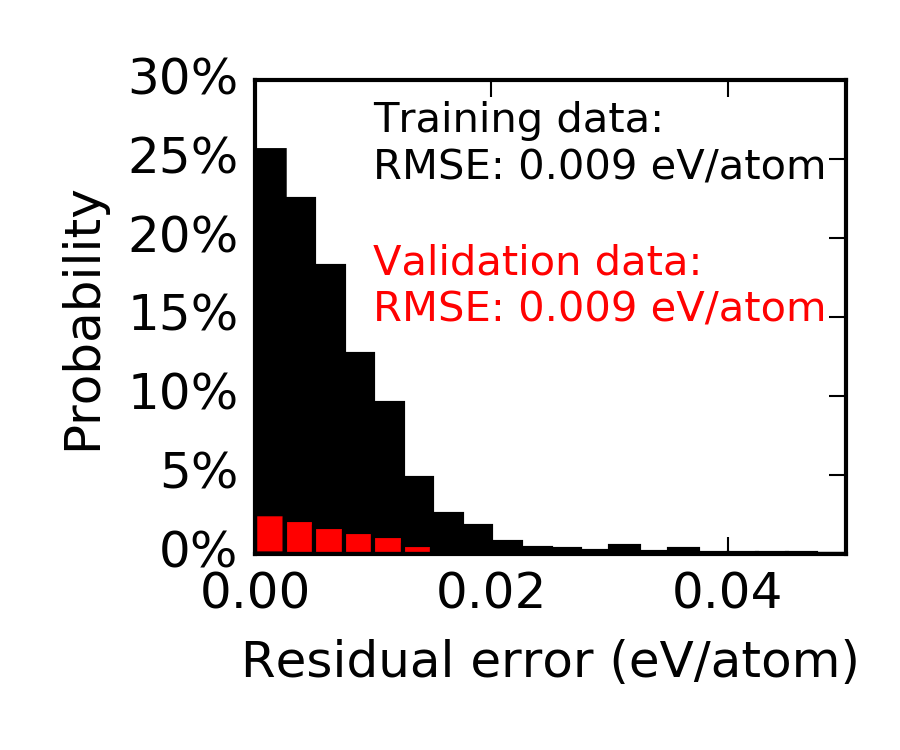
\includegraphics[width=3.5in]{./images/distribution.png}
\caption{\label{fig-residuals}
Residual errors for the energies predicted from the NN compared to DFT calculated energies. Black indicates the distribution of structures included in the training set. Red indicates the 10\% of randomly selected structures reserved for validation. The total of all validation and training points sums to 100\%.}
\end{figure}

\section{Results and Discussion}
\label{sec:orgf4fc5c0}
\subsection{Pure Pd predictions}
\label{sec:org643b6fd}
An accurate NN for bulk Pd fcc and the clean fcc(111) surface is a necessary first step before producing a NN capable of predicting oxygen adsorption on these systems. In this section, we consider the accuracy of the NN for making predictions on fcc systems constructed only of Pd. First, we consider Pd in the bulk phase. Figure \ref{fig-eos} shows the equation of state for fcc Pd. In the rest of this work, DFT predictions are shown in black while NN predictions are shown in red.

\begin{figure}[htbp]
\centering
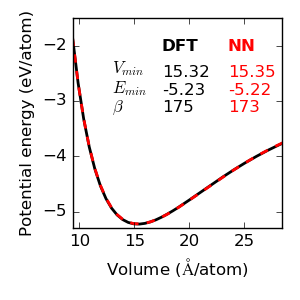
\includegraphics[width=3in]{./images/Pd-eos.png}
\caption{\label{fig-eos}
Equation of state for Pd in the fcc phase produced from fitting to volumes \textpm{} 15\% of the minimum. DFT results are shown in black while NN results are shown in red. The minimum volume (\(V_{min}\)), minimum energy (\(E_{min}\)), and bulk modulus (\(\beta\)) are also shown with units of \AA{}/atom, eV/atom, and GPa, respectively.}
\end{figure}

The equation of state was constructed from a third order inverse polynomial fit \cite{alchagirov-2003-reply-commen} to the energies from 72 calculations. Only images within \textpm{} 15 \AA{} of the minimum are considered for incorporation into the equation of state. A total of 200 bulk images were included in the available training data (\(\approx\) 1.6\% of all images). Half of the points are equation of state images, while the other half are \emph{ab-initio} MD trajectories. Even though bulk calculations make up such a small percentage of the total data, the NN predictions of the bulk equation of state are highly accurate. This can be explained by the relatively simple nature of the equation of state which can be described with a small number of variables. A summary of the bulk properties calculated in this work as well as experimental and computational references are shown in Table \ref{tbl-properties}. All results from this work are in excellent agreement with previous computational results.

Having an accurate prediction of the well-organized bulk structure will lend itself to accurate predictions of the clean slab environment. However, even before relaxations, the Pd slab will also contain new regions of the PES which include under coordinated Pd atoms that are not present in the bulk database. In this work, all slabs with adsorbates on them were constructed from four layers and the bottom two layers were held fixed. In this system, there are no Pd atoms with local environments identical to the bulk phase for a 6.5 \AA{} cutoff radius. Therefore, vacancies and low-coordinated Pd atoms are expected to play an important role in the energetics of clean and adsorbed 4 layer Pd slabs.

Next, we determine how well a clean Pd slab is represented in a NN by calculating the free energy of the surface given as: \(\sigma = (E_{slab} - n_{slab} E_{bulk})/2\). In this equation, \(E_{slab}\) is the total energy of the symmetric slab which contains \(n_{slab}\) atoms. The factor of 2 accounts for the surface at either end of the symmetric slab. Given a sufficiently large slab, the surface formation energy is then expected to converge to \(2 \sigma + n_{slab} E_{bulk}\). This convergence trend is depicted in Figure \ref{fig-surface-energy} for slabs up to 12 atoms thick. For each of these slabs, the lattice constant is fixed at the value reported in this work (See Table \ref{tbl-properties}) and no relaxation of either surface is permitted to ensure exact structural comparisons.

\begin{figure}[htbp]
\centering
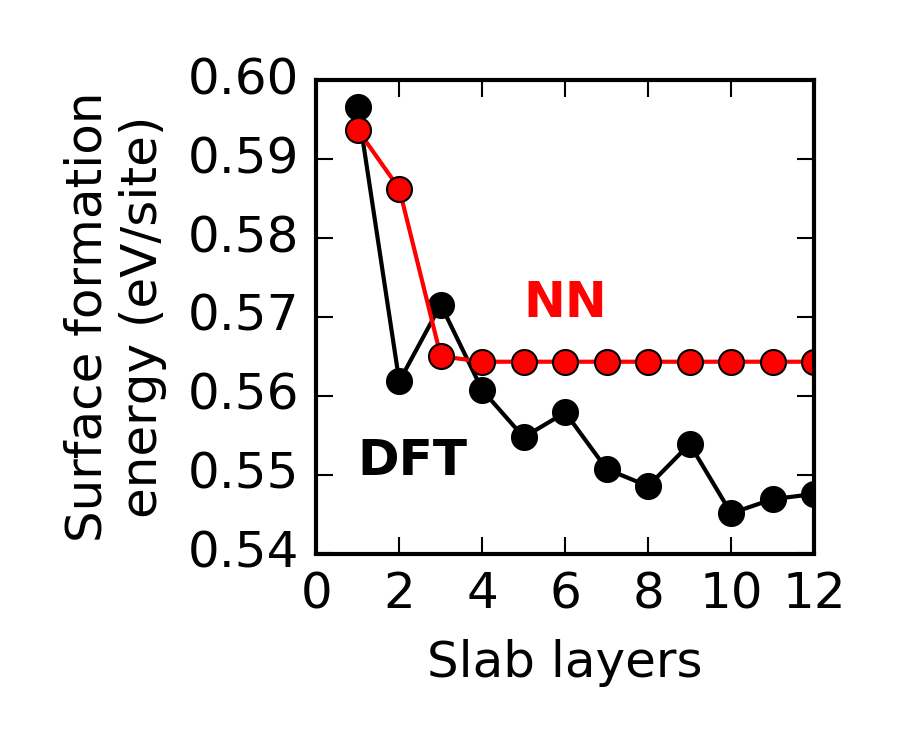
\includegraphics[width=3in]{./images/surface-energy.png}
\caption{\label{fig-surface-energy}
Predictions of the fixed surface formation energy of the Pd(111) surface with number of atoms in the slab. NN predictions are depicted by the red line while DFT is black.}
\end{figure}

For the four layer slab, the surface formation energy is estimated to be 0.561 eV/site by DFT. The NN agrees well with this result, predicting a surface formation energy of 0.563 eV/site. Comparison to unrelaxed five-layer Pd slabs from PW91-GGA are favorable at 0.565 eV/site \cite{frey-2014-implic-cover}. The small difference between the surface energy calculations of the four and five layer slabs is also suggestive that four layers of Pd is sufficient for simulating the Pd surface. This lack of convergence is a known characteristic of DFT calculated surface free energies using an incremental approach \cite{fiolhais-2003-extrac-alumin} due to non-cancellation of errors between the slab and bulk reference energies.

The lack of fluctuation in the NN predictions after four layer slabs is likely a result of the rigidity in the NNs framework in combination with a limited number of training points for this characteristic. In this training set, there are only two well-fit regions of the PES for the NN to use as reference when interpolating the surface formation energy, \emph{i.e.} clean four-layer Pd slabs, and the pure bulk Pd calculations. There are no training points from slabs of sizes other than four layers in the training set. Thus, the NN predicts that the surface formation energy of fixed atoms are converged at the four atomic layers. Since four layers is observed to be converged and only four layer slabs are used throughout this work, the inability of the NN to account for these larger slab sizes is inconsequential \emph{for this work}.

\begin{table}[h]
\caption{\label{tbl-properties}
DFT and NN predictions of various properties of pure Pd. All literature references come from Ref. \citenum{tran-2007-perfor-molec}.}
\centering
\begin{tabular}{lrrrr}
Parameter & DFT & NN & Comp. lit. & Exp.\\
\hline
Minimum bulk fcc energy, \(E_{bulk}\) (eV/atom) & -5.32 & -5.35 &  & \\
Lattice constant, \(\alpha\) (\AA{}) & 3.939 & 3.939 & 3.948 & 3.881\\
Bulk modulus, \(\beta\) (GPa) & 175 & 173 & 170 & 195\\
Surface energy, \(\sigma\) (eV/site) & 0.56 & 0.56 & 0.59 & 0.84\\
\end{tabular}
\end{table}

To perform NEB calculations, a detailed PES is required. These can be very time consuming to obtain using DFT alone since many consecutive calculations can be required, especially without a good initial guess. The NN is considerably more cost-effective than DFT, so we start by performing a very simple NEB calculation of the slipping barrier of 1 and 2 layers of Pd using the NN \cite{boes-2016-neural-networ}. Full relaxations of a 1 \texttimes{} 1 \texttimes{} 4 Pd slab were first performed for an A-B-C-A and C-B-C-A (C-A-C-A for double-layer slipping barrier) configuration using only the NN. These configurations correspond to the fcc and hcp configurations of the subsequent layers. Then, a NEB was performed over the bridge site and top site as shown in Figure \ref{fig-Pd-slipping-NEB}. After completing the NEB calculations, single-point DFT calculations were performed on each NEB image for validation.

\begin{figure}[htbp]
\centering
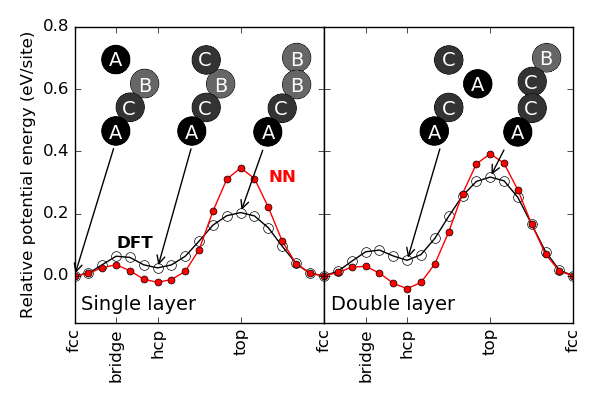
\includegraphics[width=5.5in]{./images/Pd-slipping-NEB.png}
\caption{\label{fig-Pd-slipping-NEB}
NN predicted NEB trajectory for the slipping barrier of a single layer and the top two layers of a Pd slab shown in red. DFT validated single-point calculations are shown in black. For the single layer, fcc indicates an A-B-C-A configuration while hcp indicates a C-B-C-A configuration. For the double layer transition, hcp indicates a C-A-C-A configuration of the layers.}
\end{figure}

All slipping barrier predictions in Figure \ref{fig-Pd-slipping-NEB} are made in reference to the fcc configuration as predicted by each individual method. The fcc configuration and the immediate region of the PES around it are well predicted by the NN, over-predicting compared to DFT for the same configuration by 8 meV/site. In comparison to the DFT-predicted minimum energy structure there is only a 4 meV/site difference, indicating that the NN predicted minimum is very similar in structure as well. The NN under-predicts the ground state energy for the hcp configurations by 0.04 and 0.08 eV/site for the single-layer and double-layer slipping barrier positions, respectively. The NN predicted ground state configurations differ by 0.02 and 0.01 eV/site from the DFT predicted ground state configurations. This is an indication that the NNs prediction of the A-C-A-C ground state configuration are about as accurate as that of C-B-C-A. However, the energies associated with the A-C-A-C configuration are about half as accurate.

Very few training points containing the A-C-A-C configuration exist in the dataset resulting in this under-prediction. These types of errors are naturally self-correcting in an iterative training process. Energy minimization algorithms will automatically sample these regions which are important for certain thermodynamic applications. Thus, further training iterations could be used to improve this result. The same is true for the top sites which are both over-predicted. Although the errors in the bridge to hcp region are relatively small compared to oxygen interactions, they do incorrectly-predict the hcp site to be more stable than the fcc site by 0.02 eV/site and 0.04 meV/site for the single-layer and double-layer shift, respectively. Incorporating training data of molecular dynamic simulations can also help to improve these regions since the barrier is small, leading to increased sampling of the hcp region in certain MD simulations. The SI file contains more information of how this natural sampling occurs with an example MD simulation on a 3 \texttimes{} 3 \texttimes{} 4 slab.

\subsection{Thermodynamic PdO properties}
\label{sec:org74f7c50}
First we perform DFT calculations to compute the adsorption energies (\(E_{ads}\)) of the oxygen at various coverages. We consider the energy unique configurations (as determined by EMT) of a 3 \texttimes{} 3 \texttimes{} 4 Pd slab for a total of 107 configurations. Of these structures, adsorbed oxygen is placed into the fcc, hcp, bridge, or top sites. These initial, energy unique, configurations were then allowed to fully relax and all trajectory images were added to the total dataset used to train the NN. Nearly all of the starting bridge and top site configurations relaxed into lower energy fcc or hcp positions, especially at low coverages. Adsorption energies are calculated as \(E_{ads} = (E_{slab+O} - E_{slab} - \frac{1}{2} n_{O} E_{O_{2}}) / n_{O}\). Here, \(E_{slab+O}\) is the energy of the Pd slab with \(n_{O}\) oxygen(s), \(E_{slab}\) is the energy of the clean Pd slab, and \(E_{O_{2}}\) is the DFT calculated reference energy of O\(_{\text{2}}\) in the gas phase (-8.74 eV, see SI for details).

Figure \ref{fig-PdO-thermo-coverage} shows that there is an error of about 0.05 eV/O between the NN predictions and DFT data at most coverages. All fcc configurations are consistently over-predicted by \(\approx\) 0.1 eV/O. This is most noticeable at low coverages. By contrast, hcp configurations are under-predicted by \(\approx\) 0.05 eV/O. Bridge and top site configurations are primarily relaxed into fcc configurations at low coverage and share similar levels of error. At higher coverage, structures relax into mixtures of fcc and hcp sites, resulting in errors between the two extremes. Low-coverage fcc structures represent the highest error in adsorption energy. This could be due to the fact that the single-atom coverages are not as well represented in the dataset. This is important when choosing methods for NN training data selection. Although this method is useful for omitting unnecessary duplicates, it also incorporates significantly more high-coverage calculations. For example, of the 107 images included in Figure \ref{fig-PdO-thermo-coverage}, only 4 are from single-atom coverages.

\begin{figure}[htbp]
\centering
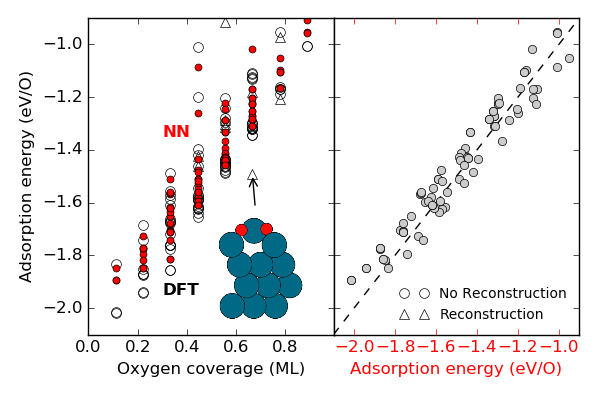
\includegraphics[width=5.5in]{./images/coverage-dependance.png}
\caption{\label{fig-PdO-thermo-coverage}
Adsorption energy of oxygen onto the surface of a 3 \texttimes{} 3 Pd slab at various coverages. On the left are the DFT calculations of the coverages (black hollow) with comparative NN predictions (red). On the right, the residual errors are shown (gray). Reconstructed structures are defined as having an average difference in the position of all atoms greater than 0.5 \AA{}. NN predictions of reconstructed structures are not shown.}
\end{figure}

At higher coverages, surface reconfigurations become increasingly common. One especially strong reconstruction is observed at 2/3 coverage. As shown in Figure \ref{fig-PdO-thermo-coverage}, two rows of oxygen on the fcc sites pull a row of Pd out of the surface, dramatically reducing the energy of the system. A similar reconstruction is observed with a single row of oxygen, but the effect on the energy of the system is not as significant. In previous work, a carbon-induced reconstruction of the Pd(111) surface was also observed at higher C coverages \cite{kitchin-2009-correl-cover}. This C reconstruction is observed on similarly sized unit cell. These reconstructions are unit cell size depended since they are not observed on 2 \texttimes{} 2 surfaces. Larger unit cells may also produce other reconstruction configurations not seen in this work. Reconstructions are also observed in MD simulations at 1/3 coverage or higher. This is consistent with previous work which shows that the Pd surface is readily oxidized at coverages above 0.5 ML \cite{lundgren-2002-two-dimen,todorova-2004-oxygen-overl}.

Utilizing the non-reconstructed oxygen predictions of the NN we can now make comparisons to previous work with cluster expansions. Frey \emph{et al.} \citenum{frey-2014-implic-cover} have produced a coverage-dependent cluster expansion of oxygen adsorbed onto the fcc site of a Pd(111) slab. Using it they predict the equilibrium coverage of oxygen on Pd under reaction conditions consistent with NO oxidation. For comparison, we have performed a similar grand-canonical MC simulation to predict the equilibrium coverage of oxygen on Pd using identical
parameters (\(\mu_{O_{2}}\) = 0.75 eV at 600 K). Since the NN (as currently implemented in Python) is more computationally expensive than the cluster expansion, a 10 \texttimes{} 10 \texttimes{} 4 Pd slab was used and no ionic relaxation was allowed. Single oxygen atoms were added/removed from the slab and an oxygen reference energy of 1/2 \(E_{O_{2}}\) was used. All simulations were started from zero coverage and allowed to run for at least 10,000 iterations to ensure good convergences across the 100 site slab. Results for a MC simulation with oxygen binding on the fcc site are shown in Figure \ref{fig-PdO-MC}.

\begin{figure}[htbp]
\centering
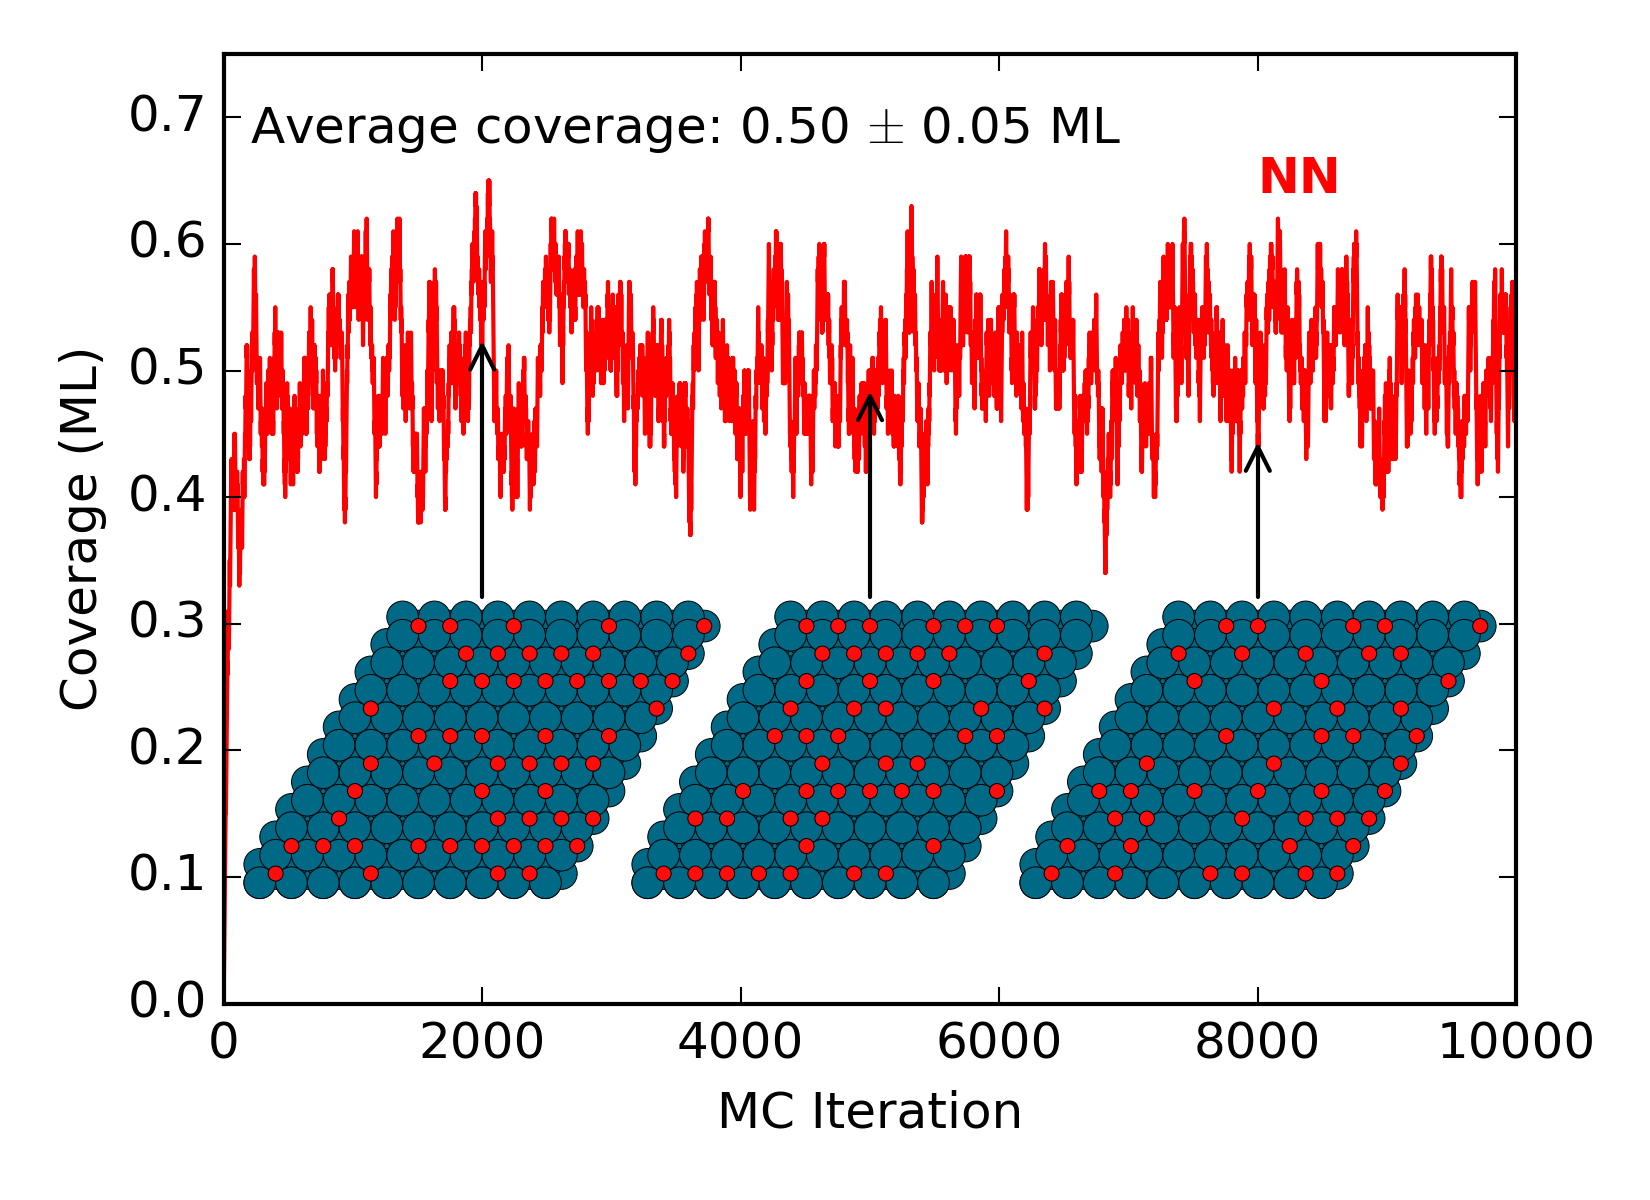
\includegraphics[width=5.5in]{./images/Pd-MC.png}
\caption{\label{fig-PdO-MC}
Grand-canonical MC simulation of oxygen adsorption a 10 \texttimes{} 10 Pd(111) surface. The simulation was run for oxygen binding on fcc sites. MC was performed with a \(\mu_{O_{2}}\) of 0.75 eV at 600 K.}
\end{figure}


The mean fcc coverage is estimated to be 0.50 \textpm{} 0.05 ML. This is 0.13 ML greater than predicted by the cluster expansion work under the same conditions. This can be explained by a difference in the predicted formation energies of the two potentials that is likely due to the O\(_{\text{2}}\) reference energy. The oxygen formation energy is calculated as \(E_{frm} = (E_{slab+O} - \frac{1}{2} n_{O} E_{O_{2}})/n_{site} - n_{slab} E_{bulk} - \sigma\). In this equation, \(n_{site}\) is the number of adsorption sites. By removing the fixed bottom surface formation energy, \(\sigma\) and and bulk energy contributions for \(n_{slab}\) atoms/site, we produce the formation energy of the oxygen covered surface on a per site basis. Comparing the trends in formation energy lends insight into the relative stability of high and low coverages. Figure \ref{fig-formation-energy} shows the oxygen formation energies of the minimum energy configurations from Figure \ref{fig-PdO-thermo-coverage}.

\begin{figure}[htbp]
\centering
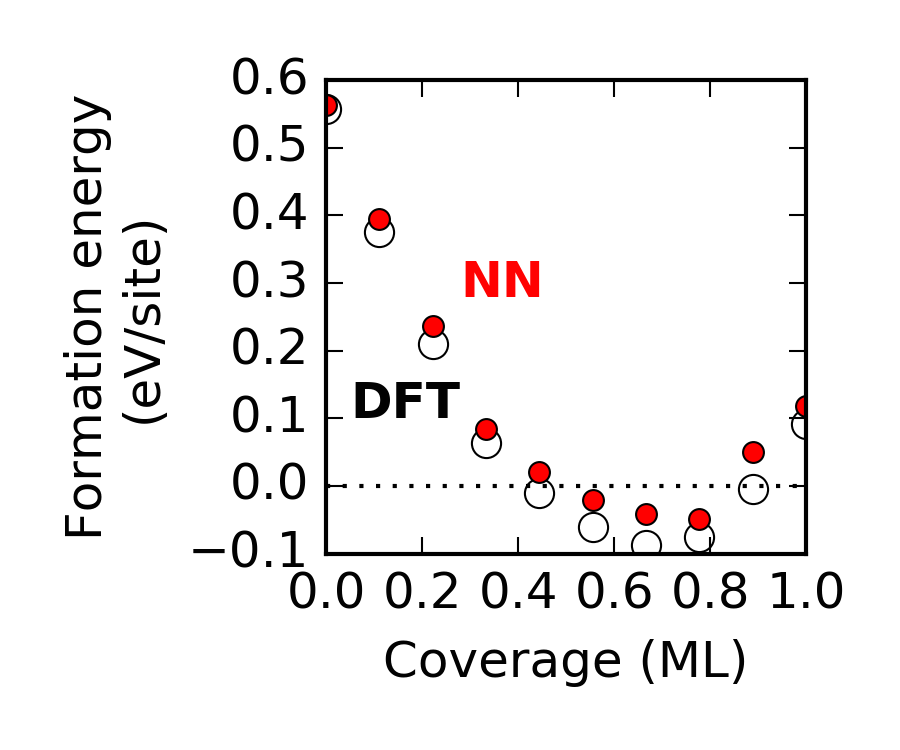
\includegraphics[width=3in]{./images/formation-energy.png}
\caption{\label{fig-formation-energy}
Oxygen formation energies on the surface of a 3 \texttimes{} 3 Pd(111) slab from 0-1 ML coverage. Fully relaxed DFT calculations (black hollow) and the NN predictions of those same geometries (red) are shown.}
\end{figure}

The point at zero coverage is representative of the surface formation energy given in Table \ref{tbl-properties}, which was shown to be in good agreement with the NN and previous work. However, the formation energies are \(\approx\) 0.1 eV/site lower at mid-range coverages and over 0.2 eV lower at 1 ML than the corresponding results from Ref \citenum{frey-2014-implic-cover}. Formation energies also drop below zero at \(\approx\) 0.45 ML. Figure \ref{fig-formation-energy} also ignores reconfigured structures which are predicted to become more stable at coverages above 0.5 ML in this work. This will result in higher coverages from the NN since it is trained to DFT results which predict increased stability at higher coverages. This trend is also highly influenced by the oxygen reference energy used \(E_{O_{2}}\). Part of this increased favorability is counteracted by the NNs tendency to over-predict adsorption onto the fcc site, but this increase is small in comparison.

The cluster expansion accounts for relaxation implicitly in its design by fitting to relaxed geometries, while the NN distinguishes between the relaxed and unrelaxed geometries. Unfortunately, performing relaxation steps between each iteration is computationally infeasible. Even with a 100\% acceptance rate, relaxing such large geometries in the serial manner required by MC is still too time consuming in the current Python implementation of the NN. Accounting for relaxation is expected to increase the stability of oxygen binding onto the surface. At low coverages, these effects are expected to be small since oxygen interaction will be minimal and the surface is fixed in a position close to the minimum energy of oxygen adsorption at the dilute limit. At higher coverages, the oxygen interactions will lead to larger relaxation effects. Thus, our model is likely over-predicting the adsorption energies at high coverages. This would lead to a suppressed mean coverage of oxygen overall. It is worth noting that cluster expansions only account for small degrees of relaxation and is unable to account for surface reconstructions which are thermodynamically favorable at high coverages. In principle a NN could accurately model reconstructions, but the one we use in this work is not trained for that.

Grand-canonical MC was also performed on the hcp sites and using the O\(_{\text{2}}\) adsorption/desorption model discussed in Ref. \citenum{frey-2014-implic-cover}. The hcp model predicts similar coverages to the fcc model which is likely due to the relative error of fcc and hcp site predictions of the NN discussed previously. Additional details of these studies along with the code used to perform the various MC simulations are included in the SI file of the published work \cite{boes-2017-neural-networ}.

\subsection{Dynamic PdO properties}
\label{sec:org6fbe687}
We use dynamic in general terms to refer to any methods which require a more complete description of the PES then just the thermodynamic minima. This includes geometric relaxations, NEB calculations, MD simulation, and all other applications which generally rely upon forces of the individual atoms. We have briefly demonstrated a few examples of these applications in the first section of the results for pure Pd as well. All simulations in this section include oxygen and are driven by the NN.

The reaction barriers for oxygen diffusion in the dilute limit are important for determining rate properties for diffusion driven surface reactions. Figure \ref{fig-PdO1-NEB} depicts the minimum energy pathways predicted by the NN using the NEB technique. Two NEBs are shown, one across the bridge site and a second across the top site. The fcc and hcp end-points are relaxed configurations of a single oxygen on a 3 \texttimes{} 3 Pd slab. Similarly, the NEB relaxations are controlled via NN predictions. All energies are taken relative to the energy of the fcc adsorption site of the given method.

\begin{figure}[htbp]
\centering
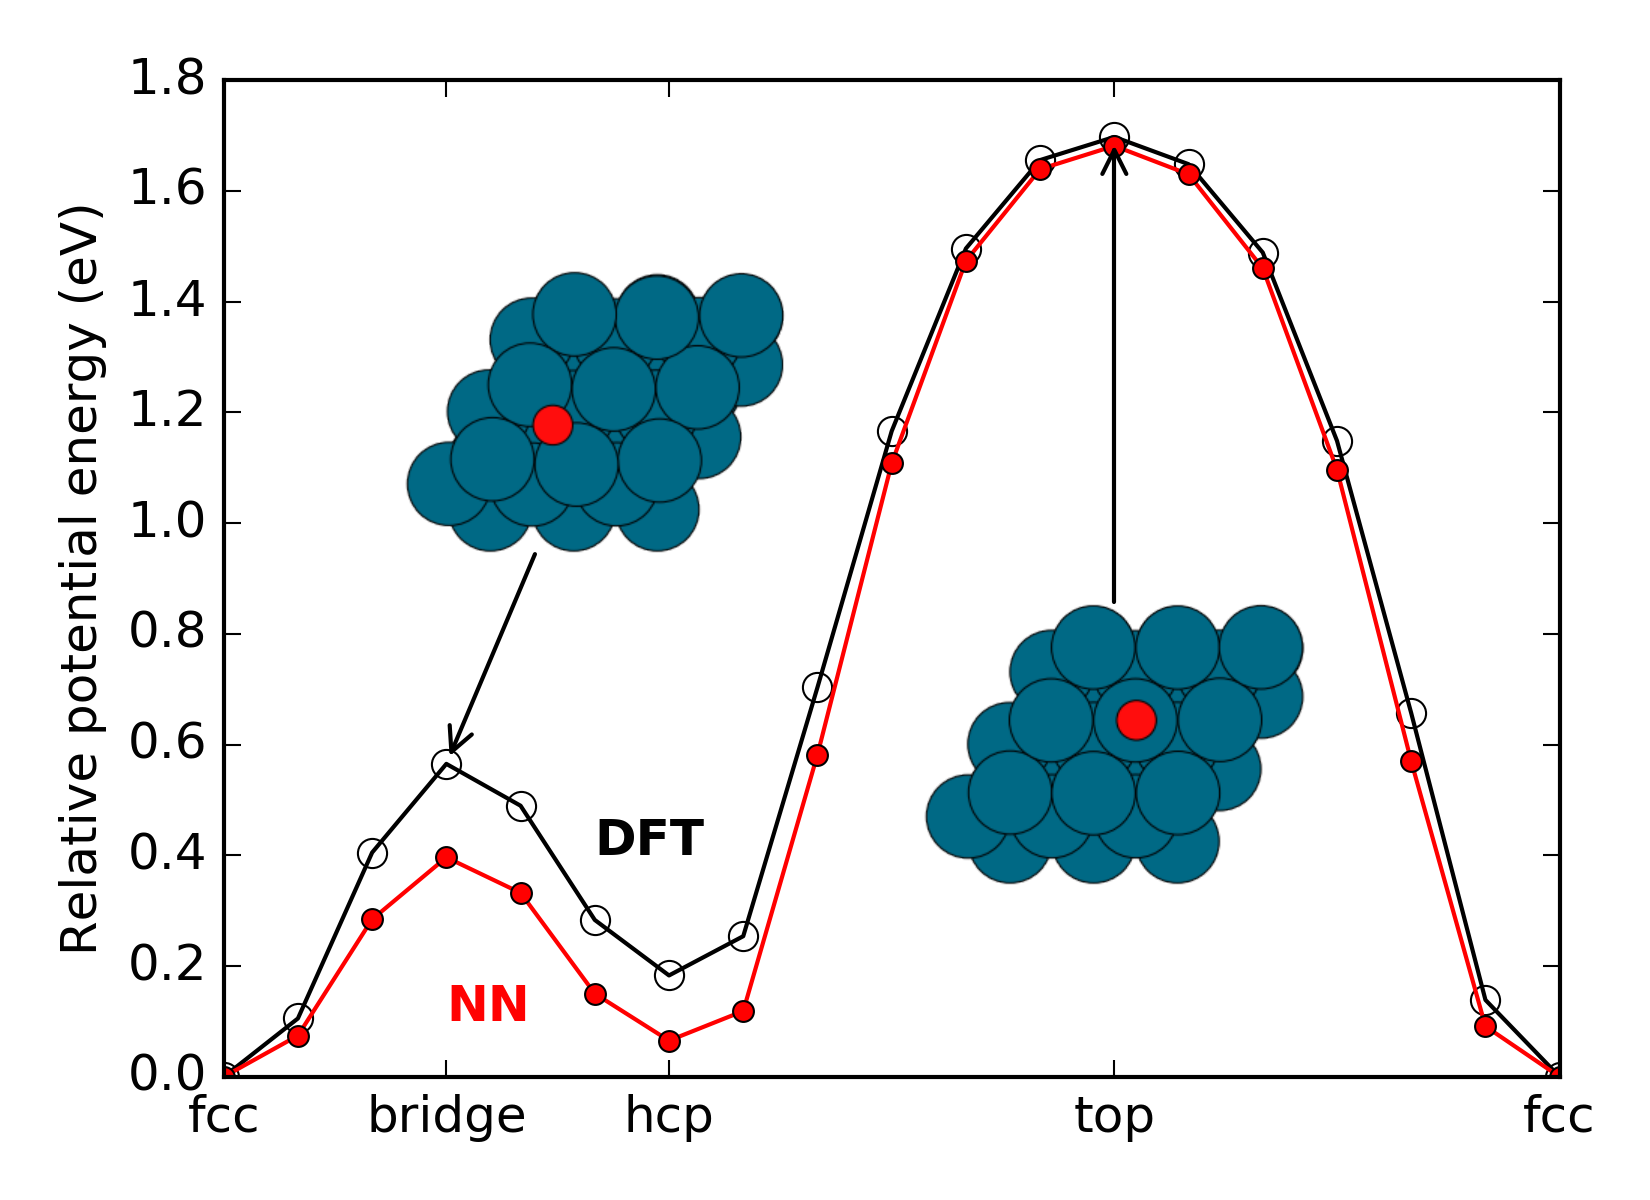
\includegraphics[width=5.5in]{./images/PdO1-NEB.png}
\caption{\label{fig-PdO1-NEB}
NN predicted NEB trajectory for one oxygen across the bridge and top sites of the Pd(111) surface. Barrier energies are taken relative to the energy of the fcc adsorption site.}
\end{figure}

The NN predicts a reaction barrier of 0.40 eV over the bridge site, while DFT predicts a barrier of 0.56 eV. Both results are in good agreement with experimental results of 0.4-0.5 eV \cite{rose-2004-chemis-atomic}. Computational results at 1 ML coverage predict a barrier of 0.37 eV \cite{markovits-2008-move-stron}. DFT validation of the relative fcc and top site energies agree very well, hcp site is under-predicted by 0.17 eV. The NN also predicts an energy difference between the fcc and hcp sites of 0.07 eV (0.18 eV for DFT) which also compares reasonably well with previous computational results of 0.17 eV at 0.33 ML coverage \cite{honkala-2001-ab-initio}. When compared to the DFT relaxation predictions in Figure \ref{fig-PdO-thermo-coverage}, the NN seems to accurately predict geometries that represent the energy minima as predicted by DFT. Although the reaction barrier over the bridge site is not as well predicted, the trends are consistent across the entire pathway, lending stability to the model.

We have also performed NEB calculations for select two oxygen atoms on the 3 \texttimes{} 3 Pd(111) surface. The path travels from minimal interaction of oxygen on the surface to adjacent fcc-hcp hollow sites. Figure \ref{fig-PdO2-NEB} depicts the NN predicted NEB pathways and illustrates the movement of the atoms across the surface.  All energies are taken relative to the energy of the fcc adsorption site.

\begin{figure}[htbp]
\centering
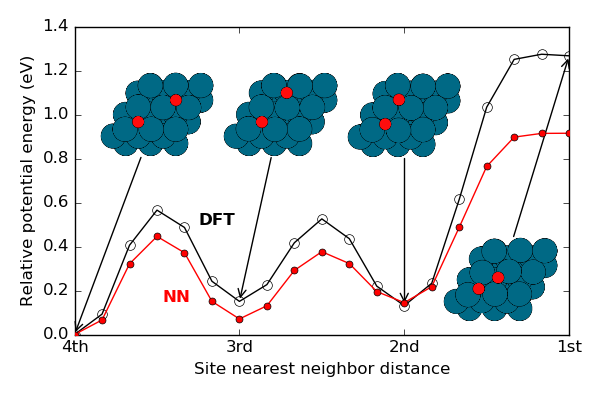
\includegraphics[width=5.5in]{./images/PdO2-NEB.png}
\caption{\label{fig-PdO2-NEB}
NEB trajectory for 2 oxygens across select sites of the 3 \texttimes{} 3 Pd(111) surface. Barrier energies are taken relative to the energy of the fcc adsorption site.}
\end{figure}

From the 4th to 3rd nearest-neighbor position, the minimum energy pathway predicted by DFT looks nearly identical with only slight increase in the energy. However, the NN over-predicts the DFT energy more than was observed with the single atom diffusion. This trend of over-prediction holds from the 3rd to 2nd nearest-neighbor site as well. Both DFT and the NN predict the 2nd nearest-neighbor site to be less stable than the 4th by \(\approx\) 0.14 eV. These results indicate a potential decrease in the reaction barrier of oxygen diffusion across the surface at mid-range coverages. As the second oxygen moves to the adjacent hcp site, a sharp increase in the energy is observed. The NN also under-predicts the DFT validation at this high coverage, which may also help explain the higher coverages predicted by the MC simulation. It can be seen in the diagram for the 1st nearest-neighbor site that both atoms are highly strained. This leads to the negligible diffusion barrier of oxygen from the 1st nearest-neighbor site to the 2nd nearest-neighbor.

We performed a MD simulation with the NN on a system sufficiently small that we could validate the results using DFT. Studies of one, two, and three oxygen atoms on a 3 \texttimes{} 3 \texttimes{} 4 Pd(111) surface are shown in Figure \ref{fig-PdO-MD}. All simulations were run at a constant temperature of 600 K and all adsorbates are started on top sites. For each simulation, every 100th step has been validated against DFT for comparison. All simulations were performed in Python using ASE. All trajectories shown can be visualized using tools available in ASE as well.

\begin{figure}[htbp]
\centering
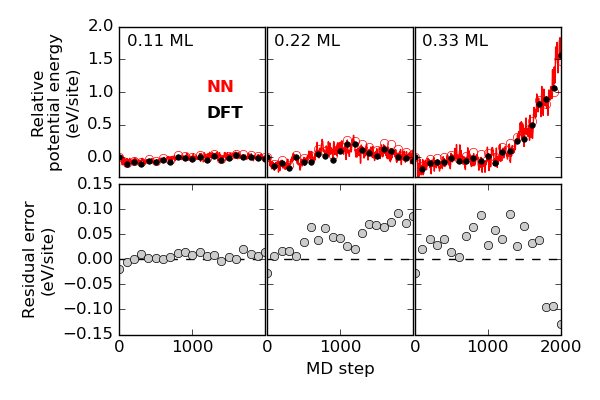
\includegraphics[width=5.5in]{./images/PdO-MD.png}
\caption{\label{fig-PdO-MD}
MD trajectories for one, two and three atoms moving across the surface of a 3 \texttimes{} 3 Pd(111). Residual errors for each simulation are shown below (gray).}
\end{figure}
For 0.11 ML, the NN performs very well over 2000 steps. No major distortion of the surface occurs. The oxygen only has enough energy to move from the fcc hollow to the hcp hollow. The initial condition has the greatest error while the rest of the trajectory is very well predicted. Occasionally, the top layer will shift into the C-B-C-A configuration, however this is likely a result of the under-prediction of the C-B-C-A configurations relative energy by the NN as discussed above. This shift of the layer is associated with a residual error decrease (\emph{i.e.} NN under-prediction) of \(\approx\) 0.05 eV/site.

For 0.22 ML, oxygen interactions result in increased diffusion of the oxygens across the surface. When moved into sites surrounding a single Pd, the surface distorts with both oxygens pulling the surrounded Pd up out of the surface. However, these distortions are not strong enough to fully dislodge a Pd atom from to top layer. Similar simulations of 2 oxygens on the surface have been performed to 10,000 MD steps with no deconstruction of the surface. For all 0.22 ML simulations, the NN consistently over-predicts the DFT energy by 0.05-0.1 eV/site. Shifts of the top Pd layer are increasingly common at this coverage.

MD simulations of coverages 0.33 ML and greater eventually fail by the NN for long MD simulations. Initially, oxygen atoms remain distant from one another, repelling each other as they get close. As the simulations progress, oxygens paired around a Pd atom in the surface exhibit similar behavior to the 0.22 ML studies, distorting the surrounded Pd out of the surface. However, these distortions are increasingly dramatic with an additional oxygen on the surface. Once the surface becomes sufficiently distorted, oxygen will attempt to move into the subsurface moving underneath the Pd. However, the potential is not trained for predictions of oxygen interactions past the top layer leading the surface to deconstruct.

A deconstruction can be seen in Figure \ref{fig-PdO-MD} for the 0.33 ML coverage. As the surface becomes more distorted, the energy begins to rise. Eventually, there is a rapid shift of the residual error trend. Quickly following this, the surface atoms will scatter. For training purposes, it is necessary to identify regions which are poorly fit so they can be added to the next iteration of the data set used for training. To avoid the computational cost of validating with DFT for all structures it is more typical to use a second NN trained with a different framework to validate results. This can be useful for selecting images which are particularly well suited for training and is a necessary first step for the automation of training a NN. An example application of this method is given in the SI file along with MD simulations run by the previous iteration of the NN to demonstrate how the NN improves its predictions with each successive iteration.

\section{Conclusions}
\label{sec:orge36def3}
We have produced a NN capable of predicting dynamic interaction between oxygen atoms on the surface of a Pd(111) slab. The NN produced was demonstrated to reproduce DFT bulk and Pd slab properties with levels of precision difficult to obtain with other types of atomistic potentials. Through incorporation of the Behler-Parrinello symmetry functions we were able to extrapolate to 10 \texttimes{} 10 slabs; large enough to perform grand-canonical MC simulations of mean oxygen coverage under reaction conditions. We predicted an average coverage of 0.5 ML at 600 K which was greater than that produced by cluster expansion work by 0.13 ML. This difference is reasonable considering the lower formation energies produced from DFT results in this work, which will favor higher coverage.

We demonstrated NEB predicted minimum energy pathways for oxygen adatom diffusion in the dilute limit as well as select pathways where two oxygen atoms interact. We observed that the NN predicts a slight decrease in the reaction barriers of mid-range oxygen interactions compared to DFT. Except for the reaction barrier of oxygen moving to an adjacent site where the reaction barrier quickly become two to three times larger. MD simulations of oxygen coverages below 0.22 ML at a constant 600 K showed good results, remaining stable and accurate to within 0.10 eV/site for MD simulations of up to 10,000 steps. At coverages greater than this, MD simulations with the NN developed in this work are prone to deconstruction before 2000 steps. This is most frequently observed as a side-effect of oxygen entering into the subsurface layer. This behavior is consistent with the known oxidation of the Pd surface at relatively low coverages.

Methods for how the NN can be improved to incorporate these reconfigurations are provided in the SI file. A significant number of additional calculations will likely be required to accurately depict oxygen interactions with the Pd surface at higher coverages, which is beyond the scope of this work. However, a large catalog of high-quality Pd and PdO DFT calculations for training are also included for application to training future potentials which seek to build off this work.

NNs are capable of representing a complete and accurate version of the PES. Although computationally expensive, machine learning techniques like the NN are still very new to the field of computational catalysis and are rapidly improving. As the techniques for creating these networks improve and large datasets of accurate \emph{ab-initio} results become widely available, we predict that the use of NNs will become as common as other fitting techniques, such as the cluster expansion.

\chapter{Modeling Segregation on AuPd(111) Surfaces with Density Functional Theory and Monte Carlo Simulations}
\label{sec:ch6}
\section{Introduction}
\label{sec:org7663464}
The effectiveness of feed-forward NNs for modeling PESs has already been demonstrated for multiple bulk systems \cite{behler-2008-press,eshet-2010-ab,khaliullin-2010-graph} as well as for Cu and Au surfaces \cite{artrith-2012-high,boes-2016-neural-networ}. They have also been demonstrated to perform well in surface calculations of H\(_{\text{2}}\)O with CuAu nanoparticles \cite{artrith-2015-grand-cu} for performance of grand-canonical MC simulations. Based on these previous studies, we hypothesized that NNs would be useful for the study of surface segregation in alloys across composition space, by enabling the use of Monte Carlo simulations of large unit cells that would provide fine-grained estimates of the surface composition, including the effects of configurational entropy and temperature on segregation.

In this work, we developed a NN trained to 3,914 DFT calculations of various AuPd alloy configurations. We demonstrate that this NN is capable of predicting energies for all alloy (111) surface configurations at lattice constants ranging from those of pure Pd to pure Au. Using this NN, we performed canonical MC simulations on relatively large unit cells of 10 \texttimes{} 10 \texttimes{} 15 atoms without surface relaxation. The mean surface compositions predicted after 20,000 successful iterations is compared to reported experimental results with excellent agreement. The MC simulation data is used to fit the enthalpy of segregation with the Langmuir-McLean formulation of the Gibbs-isotherm. We also analyze the predicted short-range ordering of the surface and discuss the reasons why surface relaxation does not appear to play an important role in AuPd segregation.

\section{Methodology}
\label{sec:org23868d6}
\subsection{Density Functional Theory}
\label{sec:org26feba4}
Monkhorst-Pack \emph{k}-point grids \cite{monkhorst-1976-special-point} of 4096 \emph{k}-points per reciprocal atom were used. The Kohn-Sham orbitals were expanded up to energy cutoffs of 400 eV for all calculations. All criteria were chosen to attain an energy convergence of at least 1 meV/atom based on studies performed on the bulk systems. The details of all DFT calculation are included in an ASE database embedded in the SI file of the published work \cite{boes-2017-model-segreg}; instructions on how to access this database can also be found in the SI, along with more details on the methods used in this Chapter.

Dilute limit segregation energies are calculated from 3 \texttimes{} 3 \texttimes{} 3 unit cells in the bulk and 3 \texttimes{} 3 \texttimes{} 5 layer surface slabs. Unit cells larger than these did not demonstrate any significant change in the dilute limit segregation energy. For each calculation, the bulk unit cell and bottom three layers of the slab calculations are held fixed at the bulk lattice constant consistent with Vegard's law \cite{denton-1991-vegar-law}. Calculations were performed for pure Au and pure Pd unit cells denoted as \(Au@Au\) and \(Pd@Pd\), respectively. Calculations of a single Au and Pd impurity were also performed in each unit cell denoted as \(Au@Pd\) and \(Pd@Au\), respectively. The dilute limit segregation energy is then calculated as: surface \(Au@Au(Pd)\) + bulk \(Pd@Au(Pd)\) - surface \(Pd@Au(Pd)\) - bulk \(Au@Au(Pd)\) for the Au (Pd) dilute limit.

\subsection{Neural Network}
\label{sec:orgc54b360}
The NNs utilized in this chapter contain two hidden layers with three nodes per layer and a hyperbolic tangent activation function. They contains two unique \(G^{2}\) symmetry functions with \(\eta\) values of one and ten. For each unique symmetry function, interactions between all permutations of the Au and Pd are included, leading to a total of eight symmetry functions. This gives a total of 66 weight variables in our NN framework. These symmetry functions are used to characterize the local environment of each atom as a single value, \emph{i.e.} one characterizing variable per symmetry function. In the symmetry functions we used a cutoff radius (\(R\)) of 6 \AA{}. A cutoff radius of 6 \AA{} was also used in the literature for Cu systems with good results \cite{artrith-2012-high}.

A database of calculations that spans the configurational and compositional space of an fcc(111) surface is required to train a NN to accurately predict segregation. To sample this space we used effective medium theory (EMT) \cite{jacobsen-1996-semi-empir} to enumerate all energy unique configurations of several slabs that were seven layers thick. A seven-layer slab was chosen because atoms in the center-most layer are fully coordinated when considering a local environment of 6 \AA{} for five lattice constants from that of pure Pd (3.934 \AA{}) to pure Au (4.154 \AA{}). Thus, local configurations with surface and bulk-like properties are incorporated for training in the NN. Depictions of these slabs are shown in Figure \ref{fig-EMT-structures}.

\begin{figure}[h]
\centering
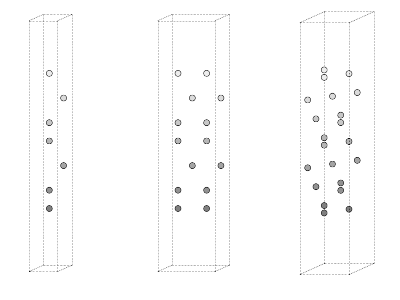
\includegraphics[width=3in]{./images/EMT-structures.png}
\caption{\label{fig-EMT-structures}
Slab structures used to enumerate energy unique configurations for NN training.}
\end{figure}

For the largest slab enumerated (\(\sqrt{3}\) \texttimes{} \(\sqrt{3}\) \texttimes{} 7), there are roughly two million (\(2^{21}\)) possible combinations of Au and Pd atoms. This was reduced to 8,405 energy unique configurations using EMT. Similarly, 4,160 unique configurations were found for the 2 \texttimes{} 1 \texttimes{} 7 structure and 72 for the 1 \texttimes{} 1 \texttimes{} 7. Each energy unique configuration was then represented at five lattice constants leading to a total of 62,706 energy and lattice unique configurations. Even after reducing the total number to energy unique configurations, the number of structures is still too large to perform a complete set of DFT calculations. Fortunately, a sufficiently trained NN should only require a small subset of these.

In total, 3,914 images were included in the complete dataset used for training and validation of the final NN. Of the overall data generated for this work 10\% was left out of the training process for use as a validation set. The RMSE of the validation set is approximately that of the training set as shown in Figure \ref{fig-distribution}. This indicates that over-fitting has not occurred \cite{behler-2015-const}. This dataset was produced from three repetitions of the iterative approach depicted in Figure \ref{fig-training-process}.

\begin{figure}[h]
\centering
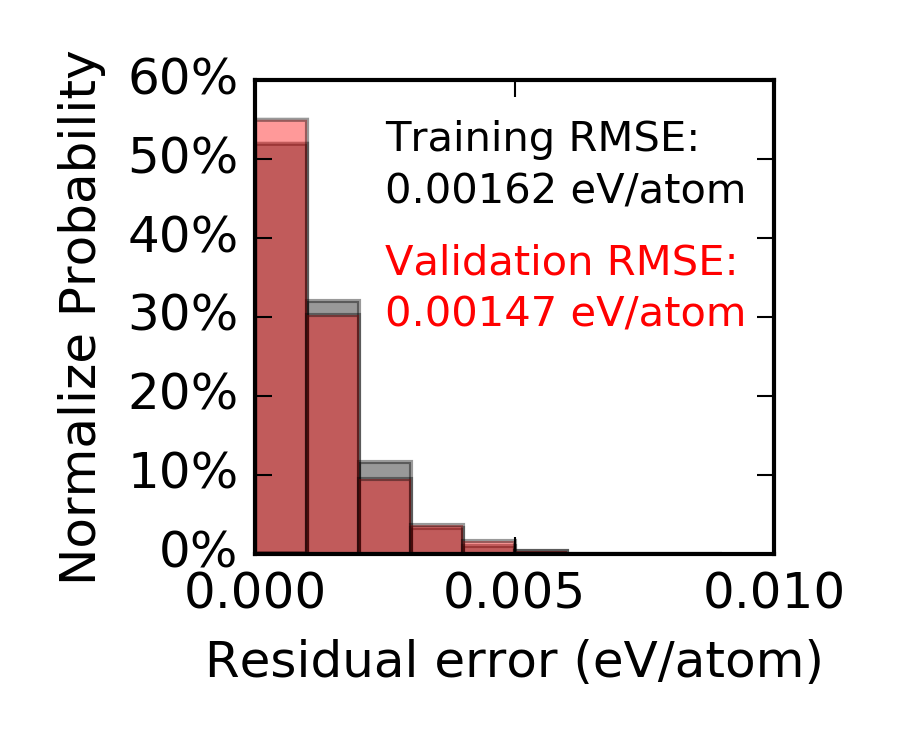
\includegraphics[width=3in]{./images/distribution-AuPd.png}
\caption{\label{fig-distribution}
Residual errors for the  difference in energy predictions from the NN and DFT. Black indicates the distribution of structures included in the training set. Red indicates the 10\% of randomly selected structures reserved for validation. Both distributions are normalized.}
\end{figure}

\subsection{Monte Carlo}
\label{sec:org0b3693c}
All MC simulations were performed using a canonical ensemble. The unit cells used were 10 \texttimes{} 10 \texttimes{} 15 slabs at varying compositions of Au and Pd. At each step of the simulation an atom of the slab was chosen pseudo-randomly and a swap with a nearest-neighbor was considered.  The change in energy for the swap was calculated by the NN and if the change is negative the swap was accepted. If the change was positive it was accepted with the usual Boltzmann probability. Relaxation energy was not considered. Discussion of the effect of non-relaxed geometries is included in the results section. The code used to perform the MC simulations is included in the SI file of the published work \cite{boes-2017-model-segreg}.

MC simulations were performed for a minimum of 20,0000 successful iterations. At an acceptance ratio of \(\approx\) 1:3 for each simulation, nearly 60,000 calculations are performed in total for each composition and temperature. On average, each atom in the unit cell has potentially been swapped at least 40 times. Since each MC simulation begins with a random distribution of the atoms, the first 5,000 successful iteration are omitted from any calculation of the equilibrium surface composition. Due to the symmetry of the slab, averages of composition in the top and bottom most layers are shown since these environments are effectively identical for the NN.

\section{Results and Discussion}
\label{sec:org8c947cc}
\subsection{Predictions of diverse local environments}
\label{sec:orgfd4b1d9}
We first demonstrate that the trained NN can accurately predict the energies of configurations that are not in the training set.  We performed an EMT enumeration of energy unique configurations of a \(\sqrt{7} \times \sqrt{7} \times 5\) slab. Only the top three layers are enumerated for this (21 atoms, \(\approx\) 2 million configurations). This allows us to effectively sample a large variety of surface configurations. Enumerations of additional layers were not included for comparison using this method since the number of enumerations grows as 2\(^{7n}\) for a binary alloy, where \(n\) is the number of layers. Thus, the next largest slab would have over 268 million configurations which is impractical to enumerate even with computationally inexpensive tools such as EMT.

The \(\sqrt{7} \times \sqrt{7} \times 5\) structure also contains multiple planes of symmetry ensuring that the number of energy unique configurations does not become excessively large. Each of the energy unique configurations determined by EMT are reproduced at the same five lattice constants as the training data. Since the bottom two layers were not enumerated, the chemical symbols of all unique configurations are also inverted from Au to Pd. Therefore, configurations on pure Pd substrates can be tested as well as those on pure Au substrates. This procedure produces a total of 546,990 energy and lattice unique configurations. Predicted energy differences between a NN with a different framework (4 hidden layers and 4 nodes per layer), and the one used for all other studies in this work, are shown in Figure \ref{fig-nn-diff}. This includes a comparison of the 62,706 configurations used in the training set to the 546,990 configurations of the \(\sqrt{7} \times \sqrt{7} \times 5\) structure.

\begin{figure}[h]
\centering
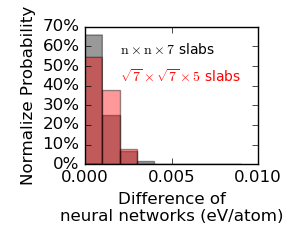
\includegraphics[width=3in]{./images/nn-diff.png}
\caption{\label{fig-nn-diff}
NN predicted energy differences for unique energy configurations. Structures from Figure \ref{fig-EMT-structures} are shown in gray while the \(\sqrt{7} \times \sqrt{7} \times 5\) structures are shown in red.}
\end{figure}

The distribution of results for a comparison between NN frameworks is partially dependent upon the flexibility of the framework, so the relative error between the two structure is important to consider along with the absolute error. The difference in NN energies for the seven layer slabs is comparable with the DFT result in Figure \ref{fig-distribution}. This is a good indication that the \(\sqrt{7} \times \sqrt{7} \times 5\) structures are well characterized by both NN frameworks. Thus, more complex configurations are likely to be well characterized.

It is possible that the small differences observed for the \(\sqrt{7} \times \sqrt{7} \times 5\) structures are a product of mischaracterization of the local environments due to too few symmetry functions. This can be difficult to determine since the fingerprints produced from the symmetry function are unique to the local environment of each atom across all images. By design, the structure types are similar, so overlap of atoms with identical local environments is expected and desirable for training purposes. It would be insufficient to simply filter all structures with non-unique local atomic environments. Instead, we produced a third NN with 40 input nodes, 2 hidden layers, and 9 nodes for each hidden layer. Such a large NN is almost certainly over-characterized for enumeration of a binary alloy slab. This large NN was used to produce segregation profiles using the same methods discussed in the following section with nearly identical results. This was taken as sufficient evidence that the energy differences shown in Figure \ref{fig-nn-diff} are not subject to mischaracterization due to over-simplification of the local atomic environments. Therefore, we are confident that the NN used in this work is accurate for all possible configurations of the local environment, and at all lattice constants of interest.

\subsection{Modeling segregation with canonical Monte Carlo simulation}
\label{sec:org4dec011}
To predict the extent of Au segregation to the surface, multiple MC simulations were performed in the 700-1000 K temperature range with bulk compositions of 0.1-0.9 Au fraction. At lower temperatures, experimental measurements of the equilibrium surface composition are not available due to kinetic limitations of diffusion. At temperatures greater than 1000 K, Au desorption has been observed leading to Pd dominated surface compositions \cite{yi-2005-compos-struc}. MC simulations were performed in increments of 100 K and 0.1 Au fraction for a total of 36 independent MC simulations. A demonstration of the surface composition for the top three layers is shown in Figure \ref{fig-AuPd-MC} at 800 K and a 50:50 composition of AuPd.

\begin{figure}[htbp]
\centering
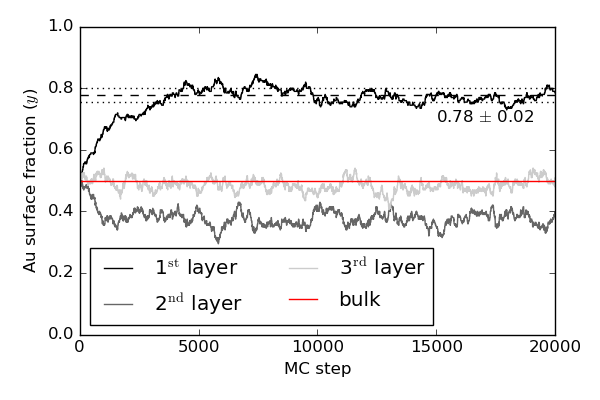
\includegraphics[width=5.5in]{./images/AuPd-MC.png}
\caption{\label{fig-AuPd-MC}
Canonical MC of 10 \texttimes{} 10 \texttimes{} 15 unit cell of 50:50 AuPd over 20,000 successful iterations at 800 K. Averages of the 1\(^{\text{st}}\), 2\(^{\text{nd}}\), and 3\(^{\text{rd}}\) layers of each side of the slab are shown.}
\end{figure}

In all 36 cases, Au segregation to the top-most surface layer is predicted. This is consistent with the experimentally measured surface energy of Au (1.626 J/m\(^{\text{2}}\)) being lower than that of Pd (2.043 J/m\(^{\text{2}}\)) \cite{mezey-1982-surfac-free}, and with Au being the larger atom. For all bulk compositions the 2\(^{\text{nd}}\) layer is observed to be Pd enriched, while the 3\(^{\text{rd}}\) layer is always similar to the bulk composition. The black dashed lines in Figure \ref{fig-AuPd-MC} depict \textpm{} 1 standard deviation around the mean surface composition.

This type of decaying oscillation of composition with layer depth is characteristic of metals with negative enthalpy of mixing \cite{dowben-1990-surfac-segreg-phenom}. Although the composition of the second layer has not been directly measured experimentally, XPS studies measure lower levels of Au segregation. This is consistent with a sub-surface region which is Pd enriched, since the XPS measurements will also incorporate some signal from sub-surface atoms \cite{yi-2005-compos-struc}. In Figure \ref{fig-AuPd-segregation} we compare our results to  experimental segregation profiles which utilize LEIS \cite{swartzfager-1981-differ-sputt,yi-2005-compos-struc}. These measurements are considered to be highly selective to the top surface composition only, which is ideal for comparison with computational results.

\begin{figure}[h]
\centering
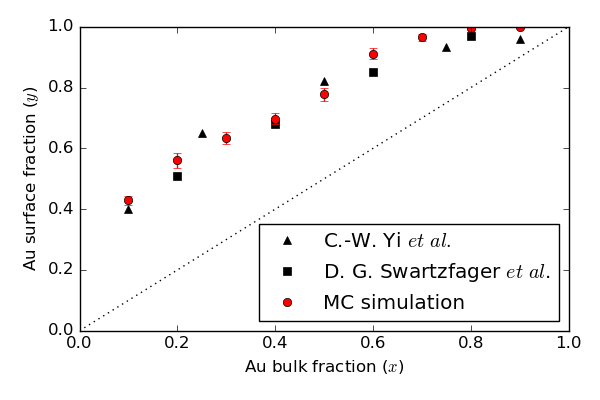
\includegraphics[width=5.5in]{./images/AuPd-segregation.png}
\caption{\label{fig-AuPd-segregation}
Segregation profile of computational results (red) at 800 K as compared to previous experimental work. Experimental studies are performed using LEIS from C.-W. Yi \emph{et al.} (Ref. \citenum{yi-2005-compos-struc}, black circles) at 800 K and D.G. Swartzfager \emph{et al.} (Ref. \citenum{swartzfager-1981-differ-sputt}, black sqares) at 875 K.}
\end{figure}

Experimental segregation energies from C.-W. Yi \emph{et al.} (Ref. \citenum{yi-2005-compos-struc}) are measured at 800 K while those by D.G. Swartzfager \emph{et al.} (Ref. \citenum{swartzfager-1981-differ-sputt}) are measured at 875 K. The computational segregation profile shown is for 800 K. Based on experimental temperature dependence studies, the segregation profile is not expected to change significantly from 800 to 875 K. In particular, an \(\approx\) 1\% reduction in composition is measured from 800 to 900 K at 50:50 AuPd bulk composition \cite{yi-2005-compos-struc}. Thus, deviations between the two sets of experimental results are qualitatively descriptive of the experimental reproducibility. Based on visual comparison, the computational results agree extremely well with the experiments. At Au bulk fractions lower than 0.6 the computational results are bounded by the expected experimental uncertainty. At bulk compositions greater than 0.6, the computational results only slightly over-predict the experimental results.

The Langmuir-McLean Gibbs-isotherm model (Equation \ref{eq-gibbs}) is used to analyze experimental data to estimate the segregation energy:

\begin{eqnarray} \label{eq-gibbs}
\frac{y}{1 - y} = \frac{x}{1 - x}e^{\left(\frac{-\Delta G}{RT}\right)}
\end{eqnarray}

\noindent where \(y\) and \(x\) are the surface and bulk fraction of Au, respectively. \(\Delta G\) can be further broken down into its enthalpy (\(\Delta H\)) and entropy (\(\Delta S\)) components as \(\Delta G = \Delta H - T \Delta S\). Due to the nature of the Langmuir-McLean equation, the \(\Delta S\) is an excess entropy term which includes only the vibrational and electronic entropy components. The entropy of mixing is accounted for implicitly within the equation itself. Since no excess entropy is incorporated into the MC simulations, this term is omitted from the fit. Using this model for the equilibrium surface composition, the enthalpy of segregation for Au can be obtained as a function of bulk composition and temperature for the alloys stable range (700-1000 K). Figure \ref{fig-temp-langmuir-mclean} shows the resulting trends from fitting to the computational results.

\begin{figure}[h]
\centering
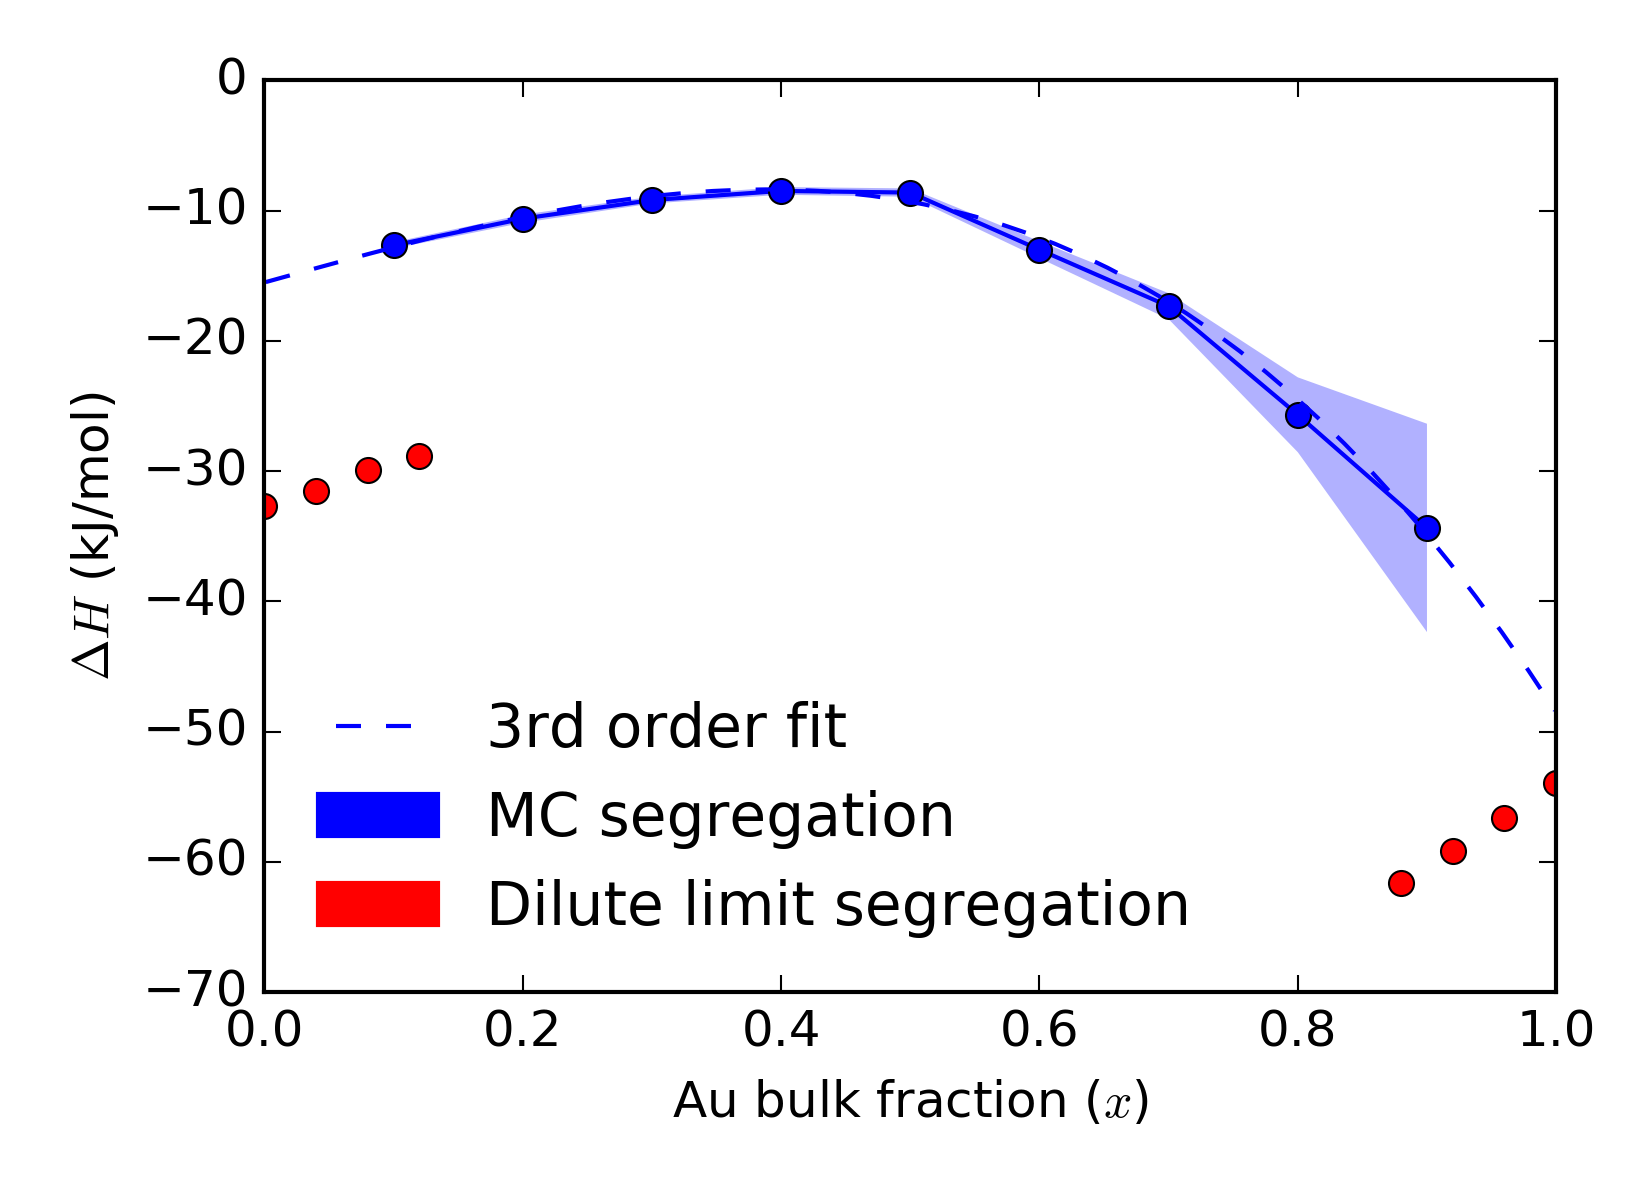
\includegraphics[width=5.5in]{./images/temp-langmuir-mclean.png}
\caption{\label{fig-temp-langmuir-mclean}
Enthalpy (blue) contributions to the Langmuir-McLean fitted segregation profile. Mean values fit to temperature dependent MC data are shown as solid dots. The shaded regions represent a single standard deviation which incorporates fitting error and uncertainty from the MC mean surface compositions. Best fits to the data are shown as dashed lines. Dilute limit segregation energies with lattice constants fixed at the corresponding bulk Au fractions are shown in red.}
\end{figure}

In Figure \ref{fig-temp-langmuir-mclean}, the fitted enthalpies are shown in blue. The shaded regions represent one standard deviation of uncertainty to the mean fitted values. The uncertainty shown includes contributions from both the fitting error as well as the standard deviation of the mean surface composition resultant from the MC simulations. As can be seen from Figure \ref{fig-AuPd-segregation}, the standard deviation of the MC-predicted surface composition is highest in the region of \(x\) \(\le\) 0.6. Despite these larger standard deviations, the majority of the uncertainty seen in Figure \ref{fig-temp-langmuir-mclean} is the result of the fitting uncertainty. This is a product of the fact that the Langmuir-McLean predictions are highly sensitive to variance in the surface composition at high Au fractions.

In the Pd rich region, the enthalpy of segregation is predicted to be relatively constant (\(\approx\) -10 kJ/mol), with the highest point at 50:50 composition. As the Au fraction increases, the segregation enthalpy begins to drop rapidly, approaching the DFT calculations of segregation in the dilute limit. This is theoretically consistent, since we expect to recover the dilute limit segregation enthalpy as we approach either limit in composition. However, this recovery of dilute limit segregation is not as apparent at the Pd rich composition end.

To see if this difference could be explained by the 10\% change in bulk composition, we performed additional dilute limit calculations with lattice constants fixed at a corresponding bulk composition as dictated by Vegard's law \cite{denton-1991-vegar-law}. The results are shown in Figure \ref{fig-temp-langmuir-mclean} as the red dots which extend between the Au fractions of zero and one. Expansion of the nearly-pure Pd lattice does indeed decrease the surface stability of dilute Au atoms, but this effect is small suggesting that Au-Au interactions likely play a significant role in the rapid deviation from dilute limit segregation predictions.

On the Au-rich end, contraction of the lattice at the nearly-pure Au lattice increases the favorability of Au replacing the lone Pd atom at the surface. This can be explained by the relatively strong energy penalty associated with moving a Pd atom to an under-coordinated surface site. When compressed, the Pd impurity increases the stability of the bulk relative to the pure Au bulk. Based on the MC analysis comparison to the dilute limit, the strain component plays a minor role compared to ensemble contributions. Also, it is clear that it would be nearly impossible to reproduce the observed trend in the segregation enthalpy from the dilute limit calculations alone.

Taking the uncertainties into consideration as weights, we have produced a 3\(^{\text{rd}}\) order polynomial fit to the segregation enthalpy data. After performing an analysis of the parameters of higher-order models, a 3rd order polynomial was found to best represent the trend with the fewest number of parameters. The equation has the form: \(\Delta H = -60.5x^3 + 27.5x - 15.5\). The second order term is set to zero since it does not contribute significantly to the fit. Further discussion of the fitted polynomial can be found in the SI file \cite{boes-2017-model-segreg}. Validation of the fitted model against the computational and experimental results is shown in Figure \ref{fig-fit-prediction}.

\begin{figure}[h]
\centering
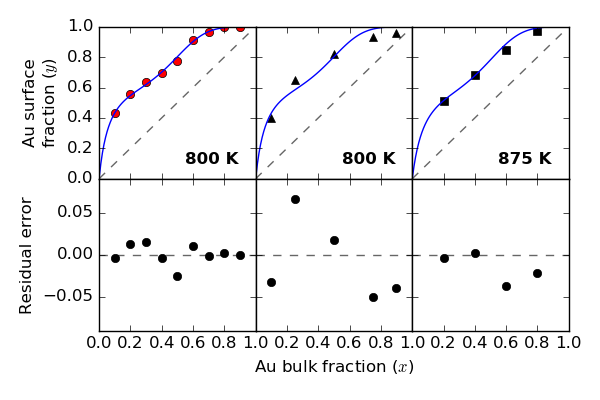
\includegraphics[width=5.5in]{./images/fit-prediction.png}
\caption{\label{fig-fit-prediction}
Langmuir-McLean fits to the computational segregation profile for AuPd. The computational results (red circles), C.-W. Yi \emph{et al.} (Ref. \citenum{yi-2005-compos-struc}), and D.G. Swartzfager \emph{et al.} (Ref. \citenum{swartzfager-1981-differ-sputt}) experimental results are shown from left to right.}
\end{figure}

The computational results (red circles), C.-W. Yi \emph{et al.} (Ref. \citenum{yi-2005-compos-struc}), and D.G. Swartzfager \emph{et al.} (Ref. \citenum{swartzfager-1981-differ-sputt}) experimental results are shown from left to right. Fits to the segregation profile show good experimental agreement at 875 K, with a maximum over-prediction of about 0.04 Au fraction, consistent with the computational results. The first data set is also fairly well represented with a maximum under-prediction of about 0.07 Au fraction. The data from C.-W. Yi \emph{et al.} can be more accurately captured with a constant -11 kJ/mol enthalpy of segregation, however this results in substantially poorer fits to the Swartzfager \emph{et al.} data. This inability for one model to capture the aspects of both experimental results is not entirely unexpected. This is most likely explained by the fact that all experimental results shown are performed on polycrystalline surfaces.

\subsection{Site distributions}
\label{sec:org1546d15}
In previous work we have utilized the distribution of sites at the surface for calculating the mean adsorption energy of H on CuPd \cite{boes-2015-estim-bulk}. In the limit of infinite temperature, the surface distribution of any set of metal atoms will become random. In this limit, the probability of finding any given three-atom site around an fcc position (\(Pr\)) can be directly related to the surface composition (\(y\)) of the alloy as shown in Equation \ref{eq-site-distribution}.

\begin{eqnarray} \label{eq-site-distribution}
Pr(y) = D \cdot y^{n} \cdot (1 - y)^{(3 - n)}
\end{eqnarray}

In this equation, \(D\) is the degeneracy of a configuration and \(n\) is the number of Au atoms in that three-atom site. The third term in Equation \ref{eq-site-distribution} is related to the probability of finding a Pd atom in the 3-atom site which can be put in terms of Au surface fraction since the total composition of all metals must sum to unity. Figure \ref{fig-AuPd-surface} shows a snap-shot of the AuPd MC simulation performed at \(x\) = 0.2 and 800 K. The surface Au fraction in this instance is 0.6. Example three-atom fcc sites are outlined for reference.

\begin{figure}[h]
\centering
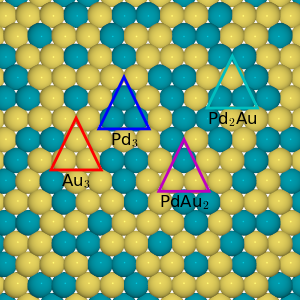
\includegraphics[width=3in]{./images/AuPd-surface.png}
\caption{\label{fig-AuPd-surface}
AuPd surface from MC simulation performed at \(x\) = 0.2 and 800 K. The Au surface fraction in this instance is 0.6. Example three-atom fcc sites are outlined for reference.}
\end{figure}

A profile of random adsorption sites can be weighted by the segregation profile to obtain site probabilities as a function of \emph{bulk} composition. However, this does not account for the possibility of short-range ordering (SRO). These SRO effects change the distribution of sites, typically towards interactions between unlike atoms for binary transition metal alloys \cite{sadigh-1999-short-range,engstfeld-2012-format-atomic}. Using the MC data we can characterize these distributions by looking at the expected composition of three-atom fcc adsorption sites. Mean values for the probability of all four possible site configurations are shown in Figure \ref{fig-site-distribution}. These configurations are sampled from the 800 K MC simulations.

\begin{figure}[h]
\centering
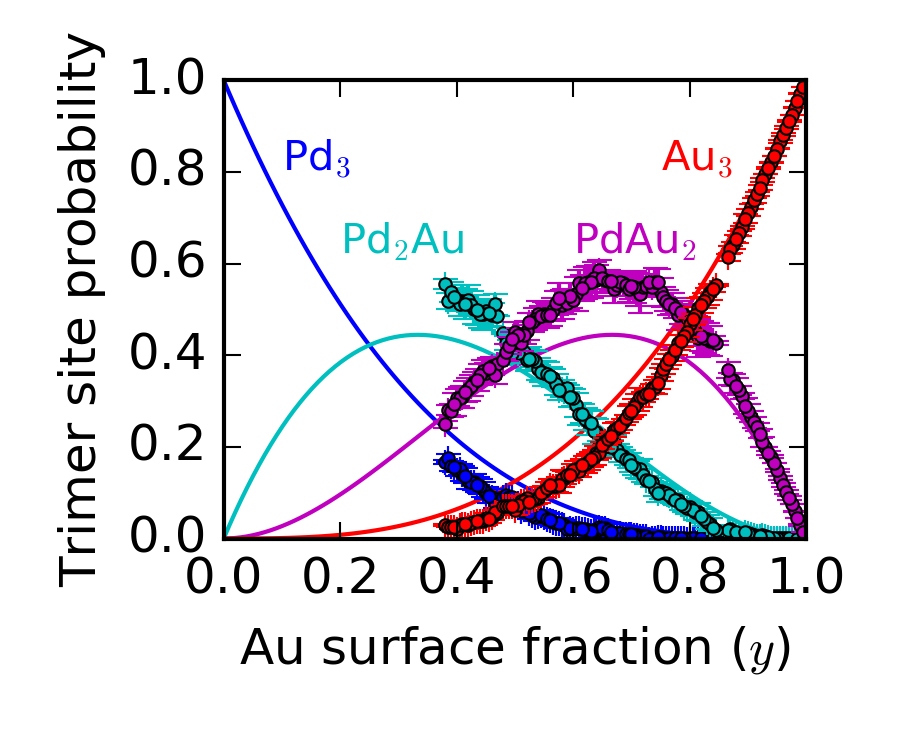
\includegraphics[width=3in]{./images/site-distribution.png}
\caption{\label{fig-site-distribution}
Three-atom fcc site distributions for all available surface compositions of equilibrated MC steps at 800 K. Solid lines denote composition of the random distribution. The circles indicate the mean distributions from the MC simulations.}
\end{figure}

For our canonical ensemble MC simulations, the surface Au fraction is not held fixed. However, as shown in Equation \ref{eq-site-distribution}, the site distributions are a function of the surface composition, not the bulk composition. Thus, each equilibrated surface was sorted by surface composition across all bulk compositions at 800 K. This method results in a more precise representation of the site distributions at any given surface composition. It also results in uneven sampling of surface compositions such as the gap in the data below \(y\) = 0.4. This gap is a product of the fact that even the lowest bulk composition sampled at \(x\) = 0.1 exhibits strong Au segregation.

The mixed Pd\(_{\text{2}}\)Au and PdAu\(_{\text{2}}\) sites are clearly favored over the pure Pd\(_{\text{3}}\) and Au\(_{\text{3}}\) sites. This indicates that there is SRO which favors Au-Pd interactions over homogeneous interactions. This is also supported by the observation that the second layer is Pd enriched which results from negative enthalpy of mixing as well. This is in good agreement with previous experimental and computational results of AuPd which show favorable heterogeneous trimer interactions \cite{sadigh-1999-short-range}.

The extent of this favorable heterogeneous SRO can be characterized with Warren-Cowley parameters (\(\alpha\)) \cite{cowley-1950-x-ray,warren-1990-x,engstfeld-2012-format-atomic}. These terms are defined generally as \(\alpha(r) = 1 - p_{AB}(r)/y_{B}\) where \(p_{AB}(r)\) is the probability of finding a \(B\) atom at nearest-neighbor distance \(r\) from any given atom of type \(A\) and \(y_{B}\) is the average surface composition of \(B\). These parameters can also be determined from multisite correlation functions in the more specific pair-wise form shown in Equation \ref{eq-warren-cowley} \cite{sadigh-1999-short-range}.

\begin{eqnarray} \label{eq-warren-cowley}
\alpha(r) = \frac{\sum_{i}\sum_{j}(S_{i} - \overline{S})(S_{j,r} - \overline{S})}{1 - \overline{S}^{2}}
\end{eqnarray}

In this equation, \(S_{i}\) is the occupation variable, for central atom \(i\), of +1 or -1 for Au or Pd, respectively. Similarly, \(S_{j,r}\) is the occupation variable of nearest-neighbor atom \(j\), with distance \(r\) from central atom \(i\). Finally, \(\overline{S}\) is the mean occupation value of the surface, related to the surface composition through \(\overline{S} = 2y - 1\). For negative \(\alpha(r)\), the \(p_{AB}(r) > y_{B}\), indicating favorable heterogeneous interaction; homogeneous interaction is predicted favorable with positive \(\alpha(r)\). At \(\alpha(r) = 0\) random surface order trends are recovered since \(p_{AB}(r) = y_{B}\). Figure \ref{fig-warren-cowley} shows calculated Warren-Cowley parameters for 1\(^{\text{st}}\)-5\(^{\text{th}}\) nearest-neighbor atoms at all available surface compositions and temperatures.

\begin{figure}[h]
\centering
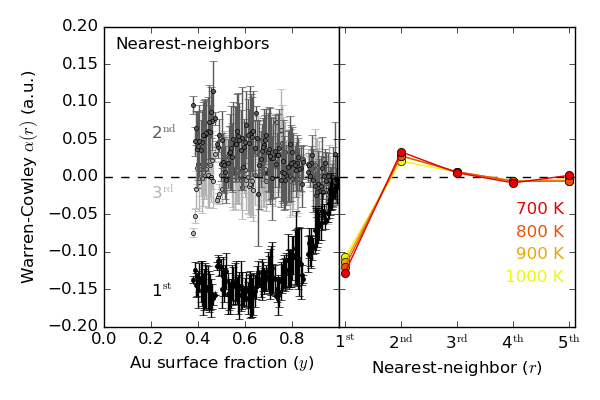
\includegraphics[width=5.5in]{./images/warren-cowley.png}
\caption{\label{fig-warren-cowley}
Warren-Cowley short-range order parameters for 1\(^{\text{st}}\), 2\(^{\text{nd}}\), and 3\(^{\text{rd}}\) nearest-neighbors as a function of surface Au fraction at 800 K are shown on the right. On the left, mean \(\alpha\) parameters are shown as a function of nearest-neighbor distance (\(r\)) for all temperatures.}
\end{figure}

On the right of Figure \ref{fig-warren-cowley}, the trends for SRO are shown as a function of surface composition for 1\(^{\text{st}}\), 2\(^{\text{nd}}\), and 3\(^{\text{rd}}\) nearest-neighbors at 800 K. The negative \(\alpha\) at 1\(^{\text{st}}\) nearest-neighbor distances indicates favorable heterogeneous interaction. The composition of the second nearest-neighbors tends to be identical to the central atom. This is also indicative of favorable heterogeneous interaction at short distances since the second nearest-neighbors are adjacent to the 1st nearest-neighbors, already identified as heterogeneously enriched. By third nearest-neighbor distance no discernible ordering effects are observed indicating no long-range interactions were observed. These findings are consistent with previous experimental and computational result giving \(\alpha(r)\) \(\approx\) -0.14, 0.04, and 0.01 for 1\(^{\text{st}}\), 2\(^{\text{nd}}\), and 3\(^{\text{rd}}\) nearest-neighbor distances at \(y\) = 0.39  \cite{sadigh-1999-short-range}. SRO effects are also predicted to rapidly diminish at \(y\) \textgreater 0.8. This is a product of the fact that Equation \ref{eq-warren-cowley} converges to zero as the surface composition approaches either pure composition.

On the left of Figure \ref{fig-warren-cowley}, the mean \(\alpha\) parameters (averaged over all surface compositions) are shown for 700-1000 K as a function of distance from the center atom. This figure more clearly demonstrates the rapid convergence of SRO effects to zero at increased distances. We can also see the rate at which the SRO effects diminish with increasing temperature. SRO effects are predicted at all of the temperatures considered in this work.

\subsection{Contributions from surface relaxations}
\label{sec:orgbadf7e3}
Performing surface relaxations between each MC step is too computationally infeasible to be performed. Despite the lack of surface relaxation, the NN driven MC simulations are in excellent agreement with previous computational and experimental results \cite{swartzfager-1981-differ-sputt,yi-2005-compos-struc}. This agreement suggests that surface relaxations do not contribute significantly to segregation or surface order for AuPd. This has not been directly studied up until this point. Previous \emph{ab-initio} predictions of the dilute limit segregation have focused on calculations made in the dilute limit to fit parameters used in an effective Ising-model \cite{creuze-2015-surfac-segreg}. Each of the terms in the effective model incorporate energies from fully relaxed DFT calculations, so there is no clear way to separate out the contribution from surface relaxation alone.

To determine why surface relaxations appear to be unimportant in determining the surface composition, we return to DFT calculations. First, we set up a unit cell of a unique 2 \texttimes{} 2 \texttimes{} 5 fcc(111) slab with 12 \AA{} of vacuum separation. A relatively small unit cell size was chosen to keep the computational expense low. Increasing the size of the unit cell allows access to increasingly disordered configurations, which are not as likely to be energetically stable. From MC simulations performed in this work, the composition of the third layer and lower is consistently predicted to be converged to that of the bulk. Based on this, the bottom three layers of the slab are held fixed at the bulk lattice constant of a 50:50 mixture of AuPd determined by linear interpolation between the bulk lattice constants of the two pure components (4.044 \AA{}). The lattice positions of these bottom three layers were then fixed to be that of the ground-state configuration of fcc AuPd.

Using this fixed basis, we use EMT to enumerate all of the unique configurations of the remaining eight atoms in the top two slab layers, as described for the NN training set in the methods section. Full relaxations of all 100 energy-unique configurations found were performed. The energies of the perfect lattice configurations were then compared to the relaxed energies. These results are summarized in Figure \ref{fig-DFT-segregation}. Formation energy calculations from the perfect lattice (blue), are representative of the energies calculated by the NN (unrelaxed). Energies for the fully relaxed systems are shown in red and the differences in the relaxed and unrelaxed energies are shown in black. The individual columns represent all 100 images separated by first layer, second layer, and total Au fraction.

\begin{figure}[h]
\centering
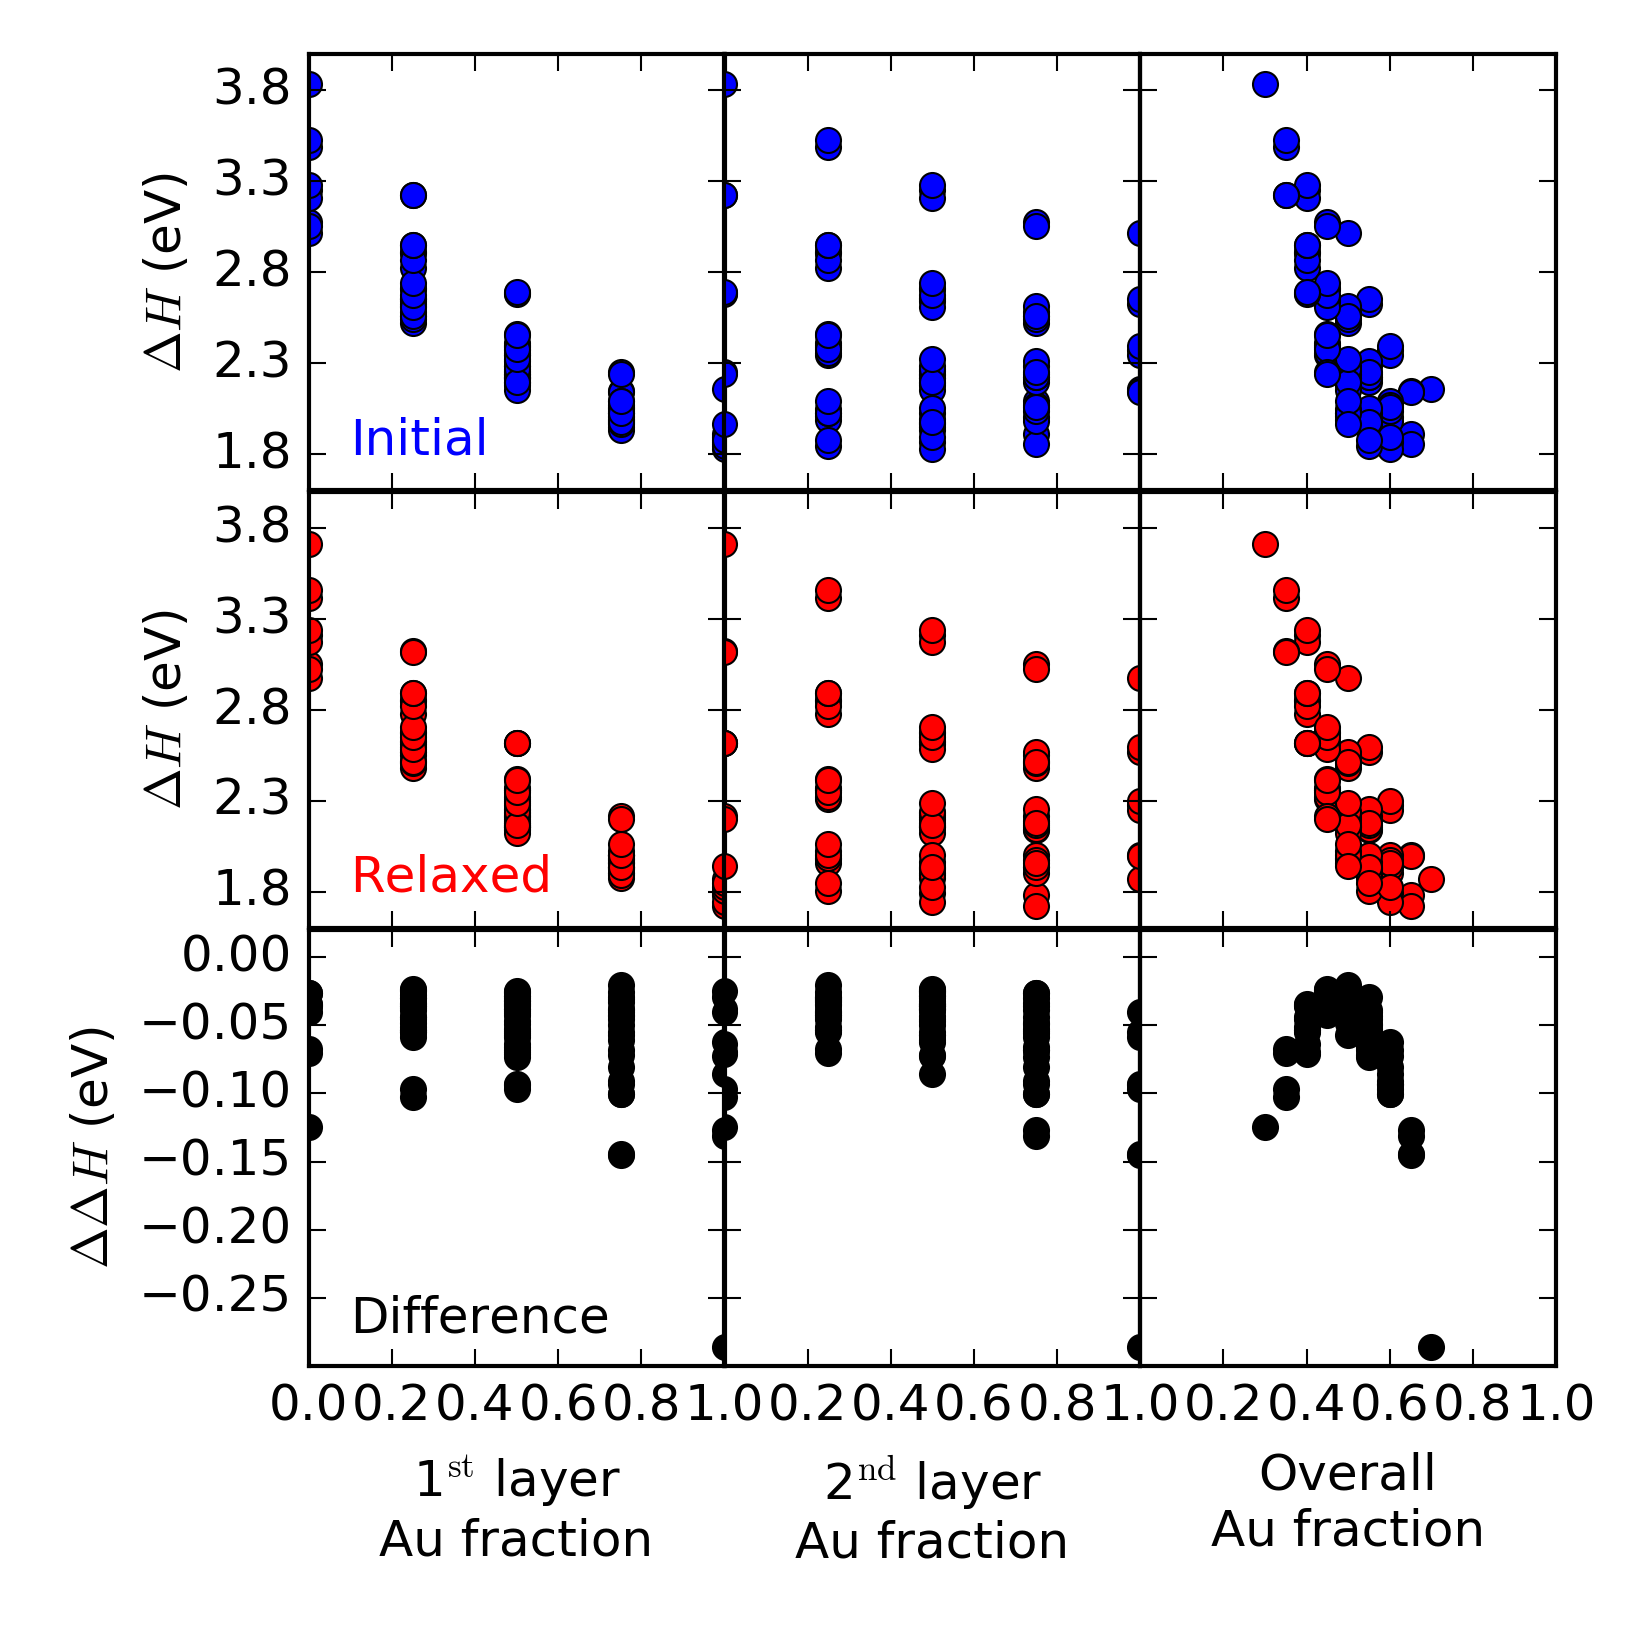
\includegraphics[width=5.5in]{./images/DFT-segregation.png}
\caption{\label{fig-DFT-segregation}
DFT energies of the symmetrically unique 2 \texttimes{} 2 \texttimes{} 5 slab of AuPd. Only the top two layers are allowed to vary in composition. Single point calculations (blue) are reflective of NN predictions, while relaxed energies (red) are those of fully converged DFT calculations. Differences between the two are shown in black.}
\end{figure}

The general trend in segregation for the unrelaxed lattice calculations reflects what is seen in the MC results predicted from the NN. Pure Au compositions of the top layer are most energetically favorable. Based on second layer compositions, the static calculations predict a more even distribution of possible stable compositions centered around \(x\) = 0.5. Compared to the relaxed calculations, these trends are mostly conserved. The biggest differences are observed in the stable configurations of the second layer compositions slightly shifting towards higher Au bulk fractions. This is also reflected in the energy differences. Most of the relaxation energies are very small in magnitude compared to the relative energy differences between compositions of the first layer. Furthermore, the relaxation energies are also very uniform, especially close to the bulk composition of the system.

The greatest relaxation energy difference occurs at the extreme ends, with the maximum occurring at a pure composition of Au in the top two layers. This is likely due to the fact that these extreme configurations prefer spacing very different from that of the predicted mixed lattice constant at 50:50 AuPd. However, even with this larger contribution in stability from relaxation, the relaxed energies are still not representative of the must stable configurations, and thus would still not be likely to be selected by MC sampling. This trend holds for all of the configurations with the greatest relaxation contributions from the perspective of the first layer composition. The influence of relaxation on the second layer composition is more ambiguous. Although higher Au compositions become increasingly stable in this case, we are also limited to considering a fixed composition of the third layer. This is likely to have a significant impact on the second layer composition which the NN driven MC is not subject to.

Overall, we observe that surface relaxations energies are relatively uniform, especially at surface compositions close to that of the bulk. Since the acceptance probability in MC simulations depend on energy differences between similar structures, this similarity in relaxation energies is expected to have little impact on the simulations. This trend breaks down for extreme differences in surface composition, but this essentially results in over-predictions in the energy of configurations which are still not energetically favorable after relaxation. Since MC is a step-wise process, energies for such extreme configurations are not expected to be sampled as frequently, if at all. Thus, it is reasonable to conclude that surface relaxations do not play a significant role for AuPd.

\section{Conclusions}
\label{sec:orgee71056}
We have trained a NN to 3,914 DFT calculations of seven layer AuPd slabs with one to three atoms per layer. Each of these slabs represent a different configuration of Au and Pd. The initial configurations were chosen with effective medium theory based on energy uniqueness. Subsequent calculations were added through an iterative process involving NN self-validation until a suitably high level of accuracy was obtained for all possible configurations of AuPd. Production of this NN allows for extensive sampling using MC which would not be feasible with DFT alone. Even with this increased computational efficiency, surface relaxation was not feasible, however it is not observed to play a significant role in this work.

Using the NN we predicted segregation profiles across composition space from 700-1000 K in 100 K intervals using canonical MC simulation. Segregation profiles predicted moderate segregation of Au to the top layer which is in excellent agreement with previous low-energy ion scattering spectroscopy measurements. Using the bulk composition and temperature dependent data we then derived the enthalpy of segregation using the Langmuir-McLean formulation of the Gibbs-isotherm. The enthalpy is well fit to a constrained third order polynomial with behavior that would be difficult to characterize from the dilute limit segregation energies alone. Finally, short-range ordering was observed due to favorable interactions between dissimilar atoms. This was quantified using Warren-Cowley parameters which are in good agreement with previous experimental results.

\chapter{Conclusions}
\label{sec:ch7}
The main objective of this dissertation has been to outline methods for the prediction of high-level reaction characteristics from, the more easily controlled, bulk composition of an alloy. In order to perform these predictions entirely from simulation, we have demonstrated that methods from multiple time scales are needed. In Chapter \ref{sec:ch2}, we demonstrated a how a course-grained thermodynamic model can be constructed which utilizes very few DFT calculations to construct bounds on the predicted adsorption energies of a single atom species at all bulk compositions. While useful for screening purposes, the accuracy of these results still requires improvement for reliable prediction of the chemistry of more complex adsorbates.

In Chapters \ref{sec:ch4} - \ref{sec:ch6}, we address these concerns by developing significantly more accurate atomic potentials for transition metals alloys than were previously available. First, these NN based potentials were shown to out-perform existing physical potentials for the prediction of Au in numerous different configurations. We then demonstrated how these NN potentials can be used to accurately represent dynamic properties of adsorbates at varying coverages, and predict segregation under vacuum conditions.

In the following section, we discuss potential future improvements to the inputs used in the course-grained approach. Many of the advancements made surrounding the NN potentials in the later chapters of this dissertation were completed with these improvements in mind. In the final section, an alternative route of advancement is discussed. This future research is based on promising integration of general machine-learning techniques for the acceleration and improvement of the methods introduced in Chapter \ref{sec:ch1}. Even beyond potential energy surface (PES) modeling, the potential for integration of machine learning techniques to assist scientists is staggering and most certainly play an increasingly important role in the future of computational catalysis.

\section{Future research for machine-learning in the simulation of alloy based reactions}
\label{sec:org18dc4a7}
The nature of course-grained models requires that they are often constructed from a long list of assumptions. These assumptions often leave the model fragile and difficult to extend to more complex chemical interactions. This can often be wholly unsatisfying, as it is often the more complex chemical reactions which we are interested in. However, until such a time that computational resources are not a concern, there will always be a need for these models. The path forward then is to consider these assumptions carefully and to find ways of eliminating those that do not scale to the problems of interest.

The model developed in Chapter \ref{sec:ch2}, represents a significant step forward in this regard. Before this point, it was not possible to directly predict an integral surface property from the bulk composition under reaction conditions. However, many of the assumptions made in the model limit its ability to scale easily to more complex reactions. Furthermore, not all of these assumptions are compatible with simulation, leaving the method incapable of being performed without experimental data. For example, it was not possible to accurately simulate the segregation profile of CuPd under vacuum conditions. Thanks to the developments in Chapter \ref{sec:ch6}, methodologies for the accurate prediction of segregation across bulk composition is now possible. However, there is still a need for more rapid techniques which are able to produce these segregation profiles accurately enough for screening many alloy compositions quickly. This can potentially be achieved using undirected machine-learning techniques for identifying the key parameters which will predict these trends across various transition metals. This will require an abundance of segregation data across multiple alloy combinations.



Another route for development is the progression towards ternary metal systems. No studies currently exist for anything other than binary metal systems at DFT levels of accuracy. This problem is largely the same as that of binary metal atoms, only the addition of a third metal adds significantly more possible configurations to be considered. Still, the process could remain largely the same as was outlined for a binary metal system in Chapter \ref{sec:ch6}. Beyond ternary metal systems, the Behler-Parrinello fingerprinting method will become increasingly expensive. Development of fingerprinting schemes which scale more readily with increasing numbers of chemical components will be required. Another promising option could be to bypass the fingerprint all together through the use of deep learning.

Along similar lines, using NN frameworks to accurately simulate single atom adsorbates on top of alloy systems is the next logical progression of the adsorbate interaction work of Chapter \ref{sec:ch5} combined with the alloy work in Chapter \ref{sec:ch6}. Again, the enumeration complexity scales as a third chemical species is added to the system. For adsorbate interactions with an alloy surface, relaxation is more likely to play an important role. As such, new techniques will need to be implemented which can account for this energy difference without needing to perform the relaxations directly. Similar concepts already exist within the cluster expansion techniques which should be adapted to machine-learning potentials for this purpose.

Finally, more advanced chemistry will require the simulation of multiple adsorbate species on the surface of an alloy slab. In this scenario, the number of possible enumerations and configurations for the system will be overwhelming. Assuming that a fingerprinting scheme capable of operating with a machine-learning potential is developed, the size of the PES would still likely be too large to bound in any systematic way. Instead, such a method would likely need to begin with previously determined sites of interest for a particular reaction. From these starting points, efficient methods for the exploration of the most relevant aspects of the PES can be implemented. Although molecular dynamics trajectories would be suitable for this purpose, the process would be terribly slow due to the current limitations of the iterative training process. Instead, intelligently designed searching algorithms, biased to avoid over sampling of already well predicted regions will be required. Once all of these steps have been completed, it will be possible to generate high-level inputs at the atomic scale for any chemical reaction of interest on a multitude of alloy surfaces.

\section{Future directions of machine-learning in computational catalysis}
\label{sec:org051ba7b}
To support the advancement of machine-learning techniques, more effective databasing for \emph{ab-initio} calculations is required. Nearly all machine-learning algorithms rely upon large input databases to perform optimally. As such, it is critically important to the users work flow that these numerous calculations not only be safely stored, but also easy to access later. It should also be designed with the intent to be useful to all computationalists in the field of surface science, as there is great potential for meta-studies in a collective database. Fortunately, all of these requirements can be easily fulfilled with existing databasing tools. It is now only a matter of taking the time to develop more convenient and novel methods for searching, and deciding upon the desired design aspects.

In the previous section, multiple potential advancements to PES implementations of machine-learning were proposed. However, the field of machine-learning has far more to offer computational catalysis than just PES representations. Unsupervised machine-learning is a category in which huge amounts of information are refined into their most important components. These techniques require the large amount of data that improved databasing techniques can help furnish. The basic concept common to these methods is that for each data point provided to the algorithm, there are many possible input variable which could describe the output variable of interest. Then, by analyzing the changes across all of the input variables along with changes in the output, the algorithm is able to infer which of the inputs are most descriptive to the selected output. The possible applications for these algorithms are quite numerous, and they are already beginning to be used for catalysis now \cite{ulissi-2017-to-addres}.

Through integration of unsupervised machine-learning techniques with supervised techniques, there is also nearly limitless potential for automation of all of the methods outlined in this dissertation; especially those of the lower time-scales where there are fewer assumptions. It is conceivable that codes could be developed in which, simply by specifying a design space of interest, a suit of machine-learning algorithms connected to an existing database would have all the tools required to self-complete any PES of interest. And of course, the possible implementations for automation and stream-lining of monotonous research tasks extends beyond PESs alone. While this is still a long way from becoming a reality, the path ahead is clear, and the future of computational catalysis, bright.

\bibliographystyle{unsrt}
\bibliography{references}
\end{document}